%
% This template has been created by:
% Pascal Bercher, pascal.bercher@anu.edu.au
%
% This is version 1.01 (13. Sep 2022)
%
% version history:
% - 1.00 (3. Dec 2021)  - first version that deserves a version number! :)
% - 1.01 (13. Sep 2022) - fixed wrong TOC link to Bibliography
%
% Make sure to use the newest version available on git!
%
% I was too lazy to put it under a specific license, but you are still free to use and alter it.
% But since I put a *lot* of effort (and experience)

\documentclass[a4paper,oneside,cleardoublepage=plain,bibliography=totoc]{scrbook}

\usepackage[a4paper]{geometry}                    % used for defining the title page

\usepackage{xurl}                                 % allows long URLs to break at any position
\usepackage[backref=page]{hyperref}               % defines style of references / links
\hypersetup{
linktocpage,                                      % in the table of contents, the numbers serve as links, not the entries
colorlinks  = true,                               % the items are colored instead of colored boxes around them
urlcolor    = cyan,
linkcolor   = black,
citecolor   = blue
}
% the following makes back references more appealing.
% Taken from: https://tex.stackexchange.com/questions/183702/formatting-back-references-in-bibliography-bibtex
\renewcommand*{\backref}[1]{}
\renewcommand*{\backrefalt}[4]{[%
\ifcase #1 Not cited.%
  \or Cited on page~#2.%
  \else Cited on pages #2.%
\fi]}




\usepackage{datetime}                             % to be able to print month & year on title page
  \newdateformat{monthonly}{\monthname[\THEMONTH]}
\usepackage{amssymb,amsthm,amsmath}               % standard math packages; often used
\usepackage{graphicx}                             % allows including graphics
\usepackage{natbib}                               % a specific citation style
\usepackage{floatrow}                             % allows to place a caption next to a figure
  \floatsetup[table]{capposition=top}             %  forces table captions to appear on top.
\usepackage{booktabs}                             % for tables that actually look nice!
\usepackage{paralist}                             % provides compactitem, a more compact itemize
\usepackage{titlesec}                             % used to add those horizontal lines around chapter package; see defs below.
\usepackage[standardsections]{scrhack}            %  fixes an error causes by loading titlesec for class scrbook
\usepackage{parskip}                              % when this is included, no indentations are used for new paragraphs,
                                                  % and instead paragraphs are separated by a small distance between them


% [requires titlesec]
% Surrounds all chapter titles by lines,
\titleformat{\chapter}[display]
{\bfseries\huge}
{\filleft\Large\chaptertitlename~\thechapter}
{3ex}
{\titlerule\vspace{1.5ex}\filright}
[\vspace{1ex}\titlerule]

% fixes a compilation errror that otherwise occurs in combination with scrbook
% see https://tex.stackexchange.com/questions/625083/adding-horizontal-line-before-and-after-chapter-heading-in-scrbook
% \titleformat{\section}
%  {\normalfont\Large\bfseries}{\thesection}{1em}{}
% \titleformat{\subsection}
%  {\normalfont\large\bfseries}{\thesubsection}{1em}{}
% \titleformat{\subsubsection}
%  {\normalfont\normalsize\bfseries}{\thesubsubsection}{1em}{}
 

 

% Set your individual data for the title page in the configuration file
% AND DONT SCREW UP THIS DATA! You should know, for example, whether it's
% an Honours thesis or not, or in which semester it is running.

% Set your name:
%  (Well, your name.)
\newcommand{\AuthorName} {Xuzeng He}


% Set the title of your work:
%  (Choose an informative and interesting title.)
\newcommand{\ProjectTitle} {Unleashing the power of Machine Learning in Geodynamics}


% Set which titlepage layout you prefer. Both provide the exact same
% information, they only differ in design to give you a bit of individuality
%  (change second line accordingly)
\newif\ifStandardTitle % do not delete this part!
\StandardTitletrue     % comment out (or use \StandardTitlefalse)
                       % to switch to an alternative title page layout


% Set the name of your school:
%  (School of Computing, School of Engineering,
%   or School of Cybernetics)
\newcommand{\School} {School of Computing}


% Set the name of your college:
%  (However your College is called.)
\newcommand{\College} {College of Engineering, Computing and Cybernetics (CECC)}


% Set your project points:
%  (6 or 12 or 24)
\newcommand{\ProjectPoints} {12}


% Set whether it's an Honours thesis:
%  (change second line accordingly)
\newif\ifHonoursThesis % do not delete this part!
\HonoursThesistrue     % or \HonoursThesisfalse or comment out


% Set your semester:
%  (S1 or S2 or S1/S2 or S2/S1 or Summer)
\newcommand{\Semester} {S2}


% Set your year:
%  (YYYY or YYYY--YYYY in case of S2/S1)
\newcommand{\Year} {2023}


% Set your degree:
%  (Whatever your degree is called.)
%  (Only required if Honours = true)
\newcommand{\Degree} {Bachelor of Advanced Computing (Honours)}


% Set your course code and name:
%  (Whatever your course code and name is.)
%  (Only required if Honours = false)
\newcommand{\CourseCode} {COMP4560}
\newcommand{\CourseName} {Course Name}


% Set name of first supervisor:
%   (Whatever her or his name is.)
\newcommand{\FirstSupervisor} {Dr.\ Alberto F. Martin Huertas}


% Set whether there's a second supervisor:
%  (change second line accordingly)
\newif\ifTwoSupervisors % do not delete this part!
\TwoSupervisorstrue     % or \TwoSupervisorsfalse or comment out


% Set name of second supervisor:
%  (Whatever her or his name is.)
%  (Only required if TwoSupervisors = true)
\newcommand{\SecondSupervisor} {%
Dr.\ Rhys P. Hawkins
\\ Dr.\ Siavash Ghelichkhan
}
                             % to specify data used in the title page

% define your own macros here

\newcommand{\Eff} {\ensuremath{\mathit{eff}}}  % example command without arguments
\newcommand{\Pre} {\ensuremath{\mathit{pre}}}  % (again)

% Note that you can easily specify arguments:
% \newcommand{\someMacro}[2] {Argument 1: #1, Argument 2: #2} % example command with two arguments
% you use it via \someMacro{Hello}{World!}


% the following commands are being provided by the amsthm package
% the first parameter states the new environmet's name that can be
% used (due to this definition here) and the second the name that
% will appear in the PDF document
\theoremstyle{definition}
\newtheorem{definition}{Definition}   % well, a formal definition!
\theoremstyle{plain}
\newtheorem{prop}{Proposition} % like a theorem, but less important or evolved
\newtheorem{lem}{Lemma}        % used within a proof of a theorem
\newtheorem{thm}{Theorem}      % well, a theorem! :) important and evolved
\newtheorem{cor}{Corollary}    % basically either a proposition or theorem,
                               %  but one that follows from another theorem.
% There's a lot you can configure about the appearance. If interested,
% open the manual of amsthm or google for tutorials etc. on that package

% the following add a symbol to the definition environment to make it more
% clear when a definition ends (as there is no difference in fonts!). From:
% https://tex.stackexchange.com/questions/226334/change-a-amsthm-theorem-ending
\newcommand{\xqed}[1]{%
    \leavevmode\unskip\penalty9999 \hbox{}\nobreak\hfill
    \quad\hbox{\ensuremath{#1}}}
\newcommand{\Endofdef}{\xqed{\blacksquare}}
\newenvironment{defn}[1]{%
    \begin{definition}#1}{%
    \Endofdef\end{definition}%
}
                                    % define all your macros here


\begin{document}

\pagenumbering{roman}

%
% This document contains two different definitions of the title page
% which one is chosen is defined in the file configutation.tex
%


% only the title page is centered; all other pages are aligned according to books
\newgeometry{left=2.5cm,right=2.5cm,top=2.5cm}
\thispagestyle{empty}

\newdateformat{monthyeardate}{%
  \monthname[\THEMONTH] \THEYEAR}


\ifStandardTitle % the first style is defined now

\noindent
\begin{minipage}[t]{6cm}%
{\footnotesize%
\raisebox{-\height}{{\bfseries The Australian National University}} \\
~2600 ACT~\textbar~Canberra~\textbar~Australia}
\end{minipage}%
\hfill%
\begin{minipage}[b]{10cm}%
\hfill\raisebox{-\height}{
\includegraphics[height=2 cm]{figures/ANU-logos/ANU_Primary_Horizontal_Black.jpg}}
\end{minipage}


\ \\[2em]
\phantom{x} \hfill
\begin{minipage}{58.75 mm}
\raggedright
\bfseries \School\\[.5em]
\mdseries%
\noindent\College
\end{minipage}\\[6 em]
\hfill

\noindent
\parbox{140mm}{\sffamily \bfseries \Huge %
\ProjectTitle%
}\\[.75 em]
{--- \ProjectPoints{} pt \ifHonoursThesis Honours \else research \fi project (\Semester{} \Year)}\\[3 em]


\ifHonoursThesis%
A thesis submitted for the degree\\
\emph{\Degree}\\[3 em]
\else%
A report submitted for the course\\
\emph{\CourseCode, \CourseName}\\[3 em]
\fi




\noindent
{\footnotesize \textbf{By:}}\\
\AuthorName\\[2em]



\noindent
{\footnotesize \bfseries Supervisor\ifTwoSupervisors{}s\fi:}\\
{\footnotesize \FirstSupervisor%
\ifTwoSupervisors\\\SecondSupervisor\fi}\\[2 em]
\vfill
{\footnotesize \monthyeardate\today}



\else % the alternative design of the title page



\begin{center}
\ \\[1em]
{\bfseries \Huge \ProjectTitle}\\[4em]
%
\ifHonoursThesis%
\Large{A thesis submitted for the degree}\\
\Large{\emph{\Degree}}\\[.5em]
{\ProjectPoints{} pt Honours project, \Semester{} \Year}
\else%
\Large{A report submitted for the course}\\
\Large{\emph{\CourseCode, \CourseName}}\\[.5em]
{\ProjectPoints{} pt research project, \Semester{} \Year}
\fi
%
\ \\[4em]
{\footnotesize \textbf By:}\\
\textbf{\AuthorName}\\[3em]
%
{\bfseries Supervisor\ifTwoSupervisors{}s\fi:}\\
{\FirstSupervisor%
\ifTwoSupervisors\\\SecondSupervisor\fi}\\[6em]
%

\includegraphics[height=2.5cm]{figures/ANU-logos/ANU_Primary_Horizontal_Black.jpg}\ \\[3em]
%
{\bfseries \School}\\
{\mdseries \College}\\
The Australian National University
%
\vfill
\normalsize{\monthyeardate\today}
\end{center}



\fi


\restoregeometry
                               % define your title page
{\sffamily\bfseries\Large Declaration:}\\

I declare that this work:\\

\begin{itemize}
  \item upholds the principles of academic integrity, as defined in the \href{https://www.anu.edu.au/about/governance/legislation}{University Academic Misconduct Rules};
  \item is original, except where collaboration (for example group work) has been authorised in writing by the course convener in the class summary and/or Wattle site;
  \item is produced for the purposes of this assessment task and has not been submitted for assessment in any other context, except where authorised in writing by the course convener;
  \item gives appropriate acknowledgement of the ideas, scholarship and intellectual property of others insofar as these have been used;
  \item in no part involves copying, cheating, collusion, fabrication, plagiarism or recycling.
\end{itemize}


\vspace{1 cm}
\hfill \monthname, \AuthorName
\newpage


% The current requirements can be found on:
% https://policies.anu.edu.au/ppl/document/ANUP_004603  (section 18) -- date: 9.2.2022
                             % includes the declaration of authorship
%\chapter*{Acknowledgements}

If you wish to do so, you can include some Acknowledgements here. If you don't want to, just comment out the line where this file is included.

There is absolutely no need to write an Acknowledgement section, so only do so when you want to -- i.e., if there's somebody you really want to thank (for example if you received extraordinary supervision). The more important the work, the more likely that an Acknowledgement section doesn't look off. In a 24 pt.\ Honours thesis it would for example look more reasonable than for a 6 pt.\ project report.\\

\textbf{Unrelated to the Acknowledgements, but important:}

\emph{Note that there exist two different title page designs.} You may choose the one that you find more appealing. Just use the configuration file to select this style. There, you also have to put in all the other information about this report like your name, the kind of report (Honours vs non-Honours) and so on.
                        % optional acknowledgements
\chapter*{Abstract}
(TODO...)                                % your abstract

% table of contents (nothing to do for you)
\renewcommand{\contentsname}{Table of Contents}   % would otherwise just be "Contents",
\cleardoublepage\tableofcontents\cleardoublepage  % which might sound less nice
\pagenumbering{arabic}

% actual report content
\chapter{Introduction}

Introduction (actually more like background) to Geoid problem and Mantle Convection (TODO...)

The rest of the paper is organized as follows. In Chapter 2, we briefly introduce the basic idea of neural networks (NN) and some specific architecture we use in this study. Some related works that use NNs to model the Geoid or mantle convection problem are also discussed in this chapter. In Chapter 3, we approach the Geoid problem using a simple fully connected neural network (FNN) and present the results. Then in Chapter 4, we present how we model the mantle convection problem by first compressing the temperature fields using a convolutional autoencoder (ConvAE) and then predict temporal evolution of the compressed temperature fields using two different Machine Learning (ML) architecture - FNN and LSTM. In the same chapter, we also discussed the difference between these two architectures by visualising the result as GIF files and applying Principle Component Analysis (PCA). In the final chapter, we conclude this paper by offering some potential follow-ups about modelling mantle convection simulations using neural networks.



                            % introduction
\chapter{Background}\label{chap:background}


\section{Neural Networks: Fully connected, Convolutional and Long Short-Term Memory}

In this section, we introduce some basic concept about neural networks (NNs) according to a more detailed explanation provided by Bishop. \citep{10.1117_1.2819119} A simple NN usually consists of one input layer, one output layer and one or more hidden layers in between. Multiple nodes inside each layers are called neurons. 

A feedforward Fully Connected Neural Network (FNN) using linear layers for connection (the term “fully connected” means that the neurons in each layer have a connection to all neurons in the previous layer and also the following layer) can be represented as a parameterized function \citep{2306.06304}, here denoted $\mathcal{N}(\theta)$, and defined as the chained composition of $n$ affine maps $\Theta_i$ (i.e., $n$ hidden layers) and activation function $g$:

\begin{equation*}
\mathcal{N}(\theta) = \Theta_n \circ g \circ \Theta_{n-1} \circ \ldots \circ g \circ \Theta_1,
\end{equation*}

where $\theta$ represents the set of all trainable parameters.

The affine maps can be defined as:
\begin{equation*} 
\Theta_i(x) = xA_i^{T} + b_i, \ \mathrm{with} \ i=1,\ldots,n, 
\end{equation*}

where $A_i$ and $b_i$ are the weight matrix and bias vector, respectively, corresponding to the $i$-th hidden layer.

Both $A_i$ and $b_i$ are able to be optimized through a technique called error backpropagation, where we first define a loss function to calculate the loss value (error) between the predicted output from the output layer and the actual output from the dataset. The error is then propagated backwards through all the hidden layers using the chain rule to perform differentiation. Eventually, these derivatives of errors with respect to the weights are used to update the learnable parameters ($A_i$ and $b_i$) in each hidden layer. This complete process is called gradient descent. 

By looping over the process of feeding the input data into NN to perform prediction, calculating the loss between the prediction and the actual data and eventually using the loss value to optimize the learnable parameters in each layers, the NN model is able to be adjusted to a state that best fits the underlying pattern of the provided dataset given its current structure.

In this study, we use a ML library called PyTorch to implement the NN architecture, specifying the loss function and optimizer that minimize the loss function (Adam optimizer, in this case, is used throughout the study due to its broader adoption for deep learning) and systematically train and test the performance of the networks.

Apart from FNNs, Convolutional Neural Networks (CNNs) are also one of the most commonly used NNs. They can handle matrix or image input better than the traditional FNN with linear layers. Instead of linear layers, they use convolutional layers that contain specified numbers of trainable filters, each of which is used to enhance or identify a particular feature in the input. Filters are convolved with the input image or the output of the previous layer, and the results are summed together along with a trainable bias and passed through an activation function to produce a feature map. Similar to FNN, activation function is also added to introduce non-linearity to the feature map.

In this study, a variation of CNN is used as a way to compress the size of the input data in the mantle convection problem, which is called Convolutional AutoEncoder (ConvAE). It is constructed as two separate sturctures that are trained together: an encoder using convolution operation to reduce the size of the original input and output a latent space representation, and a decoder using deconvolution operation to transform the latent space representation back to its original size. By feeding the input into a ConvAE, the dimension of the original high-resolution input can be decreased with the main features captured (some information may be lost during the encoding process), thus making it more computationally efficient to work with if we want to feed it into a prediction NN.

Since the dataset in the mantle convection problem is a time sequence with adaptive timestamps, long short-term memory (LSTM) is used to predict a sequence of output apart from FNN. LSTM's architecture that use a sequence of input recurrently during prediction allows it to handle time-series data more accurately than other networks since it uses a set of inputs from previous time-steps to predict the outputs at the next set of time-steps, thus leading to a potential better result.


\section{Related works for solving geoid and mantle convection using Neural Networks}

Neural networks has been increasingly used for studying the geodynamics nowadays, especially when it comes to solving geoid or mantle convection simulation. 

For example, Kerl provide a bold attempt at using ML as a low-cost solution to the geoid inverse problem in his thesis, where two separate solutions using different number of CNNs are compared.\citep{kerl2022geoid} He found that the single network solution where a radial viscosity profile is predicted directly from the geoid and density data allows him to obtain a smooth, long-wavelength estimate of the Earth’s radial viscosity profile. This provides us some implications on using only one NN to solve the inverse problem instead of stacking NNs together.

As for the mantle convection problem, a group of researchers \citep{10.1093_gji_ggaa234} make use of the FNN architecture to build a surrogate model that can predict the entire evolution (0–4.5 Gyr) of the 1D temperature profile of a Mars-like planet for a wide range of values of five different parameters, including reference viscosity, activation energy and activation volume of diffusion creep, enrichment factor of heat-producing elements in the crust and initial temperature of the mantle.

In another study that is particularly worth highlighting, Agarwal and other researchers extend their previous approach \citep{10.1093_gji_ggaa234} of using FNN trained using a large number of 2D simulations to predict the evolution of entire 1D laterally-averaged temperature profile in time for complex models. Instead of predicting 1D temperature field, the full 2D temperature field are predicted since it could contain more information related to the structure of the convection.\citep{10.1103_physrevfluids.6.113801} To show that NN techniques can produce reliable parameterized surrogates, they first use ConvAE to compress the size of each temperature field by a factor of 142 and then use FNN and LSTM to predict the compressed fields. They discovered that LSTM capture the flow dynamics better than FNN despite the fact that LSTM has a lower mean relative accuracy. Their study provides us some essential insights in solving the mantle convection problem by using NNs as a low-cost solution, including using ConvAE to compress the data and compare the prediction result of two different architectures (FNN and LSTM).

Overall, previous works have explored the usage of Convolutional Neural Networks (CNNs) to solve the inverse geoid problem directly \citep{kerl2022geoid} or FNNs/LSTMs to approximate the forward mantle convention problem \citep{10.1103_physrevfluids.6.113801}. 

In contrast to these works:
\begin{itemize}
    \item We use FNN on 1D spherically symmetric viscosity model to solve the forward geoid problem as a first step to solve the inverse geoid problem.
    
    \item We aim to produce the complete mantle convection time-series from an initial temperature field, rather than the next time-step out of the previous ones for a given set of parameters of the mantle convection model.
\end{itemize}
                              % background/framework
% \chapter{Related Work}\label{chap:relatedWork}

                             % related work
\chapter{Geoid problem}\label{chap:content}

Geoid, in the field of geodynamics, represents the shape of a gravity equipotential across the whole of Earth's surface. Detailed maps of geoid elevation with contours spaced as close as 1m can show the effect of tectonic features such as deep sea trenches, outer arc rises, and oceanic ridges and troughs on the height of the geoid, which could provide powerful constraints that must be satisfied by the next generation of geodynamic models along with other data such as high quality determinations of surface deformation and new high resolution seismic data. \citep{10.1038_299104a0}

Geoid, as shown in the Figure \ref{figure:geoid_factors}, is generally related to both the 3D density field of the Earth and the radial viscosity profile of the Earth's mantle. However, a recent research shows that modelling that treats the geoid as being purely based on density variation near the surface can poorly explain the accurately observed geoid measurements with a satellite. \citep{10.1098_rsta.1989.0038}

Therefore, in this research, we aim to use Neural Network as a way to forward model the geoid problem,
assuming that viscosity varying in the radial direction with depth is the most important factor.

\begin{figure}[H]
    \centering
    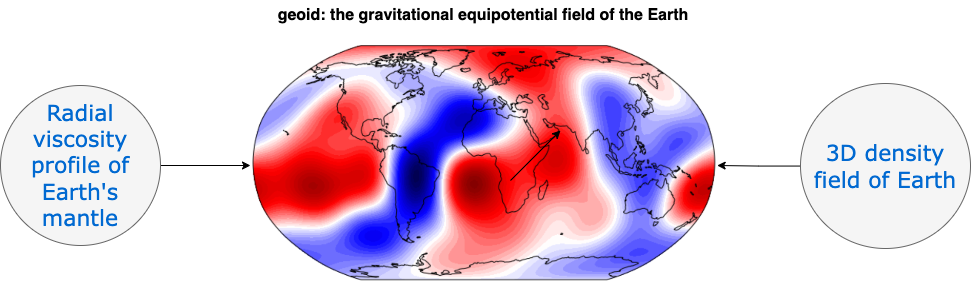
\includegraphics[scale=0.4]{figures/geoid_images/Geoid.png}
    \caption{Geoid and its two related factors.}
    \label{figure:geoid_factors}
\end{figure}

To explore the usage of Earth’s viscosity to model the geoid using NNs, we use a 1D spherically symmetric viscosity model to compute a geoid surface in terms of some spherical harmonics coefficients that can be used to construct the geoid surface. To further simplify this problem, the dataset used for this research uses a reduced prior such that the perturbations to the output are smaller.


\section{Dataset of geoid prediction}

The reduced dataset consists of 1000 pairs of input and output. In the dataset, input is a vector with 257 values indicating a 1D spherically symmetric viscosity model and output is a vector with 60 values representing a set of spherical harmonic coefficients describing the geoid height on the surface of the Earth. Figure \ref{figure:geoid_sample} here is a sample geoid field constructed from a random set of 60 geoid coefficients from the output data, where the units of the geoid are in metres and represent values greater or less than some reference value.

\begin{figure}[H]
    \caption{Sample geoid field, where the units of the geoid are in metres and represent values greater or less than some reference value.}
    \label{figure:geoid_sample}
    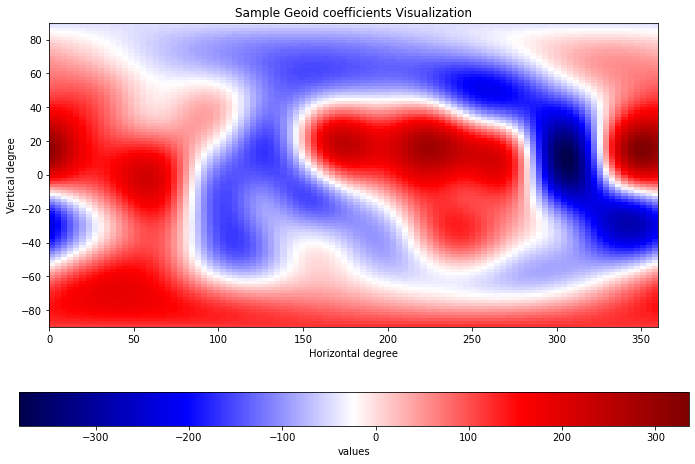
\includegraphics[scale=0.6]{figures/geoid_images/Geoid_Sample_visualization.png}
\end{figure}

To further observe the patterns in the input and the output, 10 pairs of input and output are plotted in Figure \ref{figure:geoid_input} and Figure \ref{figure:geoid_output}.

\begin{figure}[H]
    \caption{Every 100th input in the dataset.}
    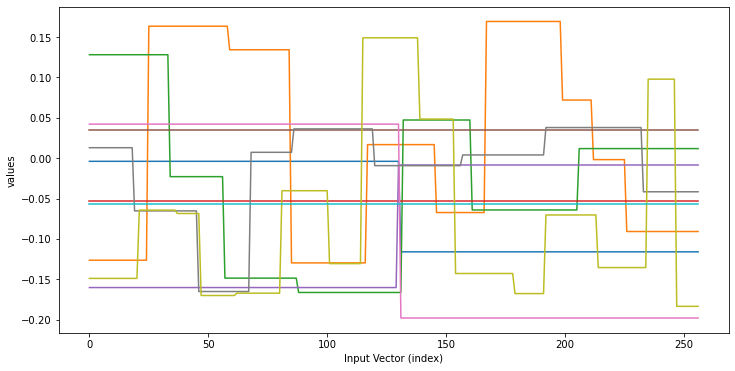
\includegraphics[scale=0.6]{figures/geoid_images/Geoid_sample_input.png}
    \label{figure:geoid_input}
\end{figure}

\begin{figure}[H]
    \caption{Every 100th output in the dataset.}
    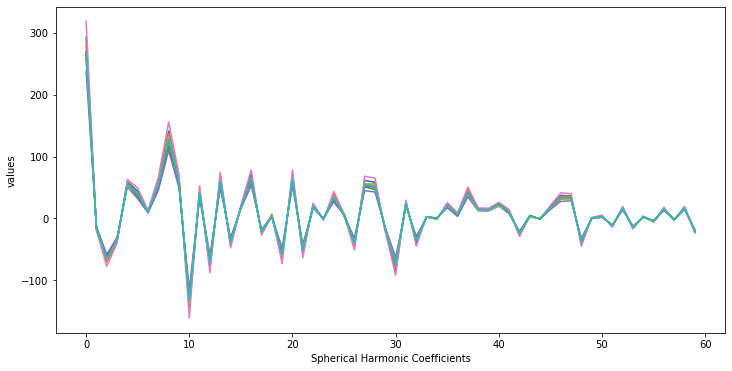
\includegraphics[scale=0.6]{figures/geoid_images/Geoid_sample_output.png}
    \label{figure:geoid_output}
\end{figure}

From the second plot we can observe that the outputs in the dataset can be seen as some "curves" with the same patterns but with different amplitude. In this case, each of the 60 coefficients in the output data are normalised to be between 0 and 1 using their maximum and minimum values separately before feeding into the neural network. This is because each of the parameters in an output vector can be seen as equally important and we want to prevent the neural network from spending most of its effort learning the parameter with a higher range of values. Hence, one can expect a higher accuracy when the parameters in the output data are standardized to the same range.

After the output data is normalised using a scalar, the entire dataset is randomly divided in a ratio of 8:1:1: 80 per cent of the dataset is used for training, 10 per cent of the data for testing accuracy and the remaining 10 per cent to perform validation during training and prevent overfitting. For a dataset with 1000 samples, this result in a train-test-valiadation split of 800-100-100.


\section{Fully Connected Neural Network for Prediction}

To test feed-forward fully connected neural network (FNN) with different architectures (e.g. different number of hidden layers and neurons per hidden layer) or other sets of hyperparameters (e.g. optimizer), a systematic testing method is applied. This method mainly consists of three files: one text file to store all the different set of FNN architectures and hyperparameters in a text format, one Jupyter Notebook file to fetch all these combinations of architectures and hyperparameters line by line, build them as FNN models and train these models, and another Jupyter Notebook file for testing and visualisation of the trained models by specifying the path of a trained model.

The trained FNN architecture (in the format of a light-weight file) along with another text file contains the training loss and validation loss during training will be stored in a specified path for further testing and visualisation. The name of these two files uniquely defines each experiment by including the values of hyperparameters used to generate this model in the file names. These files are also put in separate folders with the folder name associated with commit IDs to handle tracking of the process during the research in an educated or extensible way.

In this way, one can open the same Jupyter Notebook for testing in different browser tabs, and then visualize simultaneously different models in different tabs using a cell in which the paths to the FNN model and its training data are specified. 

The systematic testing capability is implemented here to ensure traceability. In other words, as different values of the hyperparameters are tested, We would like to be able to record the results (e.g., the trained network and the training data) so that we don't have to repeat them again or rely on our memory to compare the the performance of different structures.

Also, to prevent overfitting, a variation of the early-stopping method is used during training. The normal early-stopping method let the network train until the error function evaluated on the validation set starts to increase beyond a certain threshold \citep{10.1007_978-3-642-35289-8_5}, while my implementation only stores the best model during training (the one with the lowest validation loss) in a specified path and allows the network to keep training as normal. In this case, the output model is the best model instead of the last trained model. This method is also used in the upcoming chapters when implementing the ConvAE, FNN and LSTM to solve the mantle convection problem.

After testing with NNs with different number of hidden layers and neurons per hidden layer, we found that FNN with a total number 3–4 hidden layers seemed to perform the best.

In the following figures, we present results from a FNN with 4 hidden layers with 200, 160, 120 and 80 neurons, ReLU as activation function, MSELoss as loss function, and trained for 200 epochs using Mini-Batch Gradient Descent (with a batch size of 16).

One thing to notice is that the loss value, which is back-propagated during the training process, is calculated using the prediction and the normalised output. In this case, the best case and the worst case shown as below are also defined upon the value of this normalised error in order to be consistent, including the training loss and validation loss in Figure \ref{figure:geoid_losses}, the overall testing result in Figure \ref{figure:geoid_testing},  the most accurate geoid prediction in Figure \ref{figure:geoid_best} and the least accurate geoid prediction in Figure \ref{figure:geoid_worst}.

\begin{figure}[H]
    \caption{Training loss and Validation loss.}
    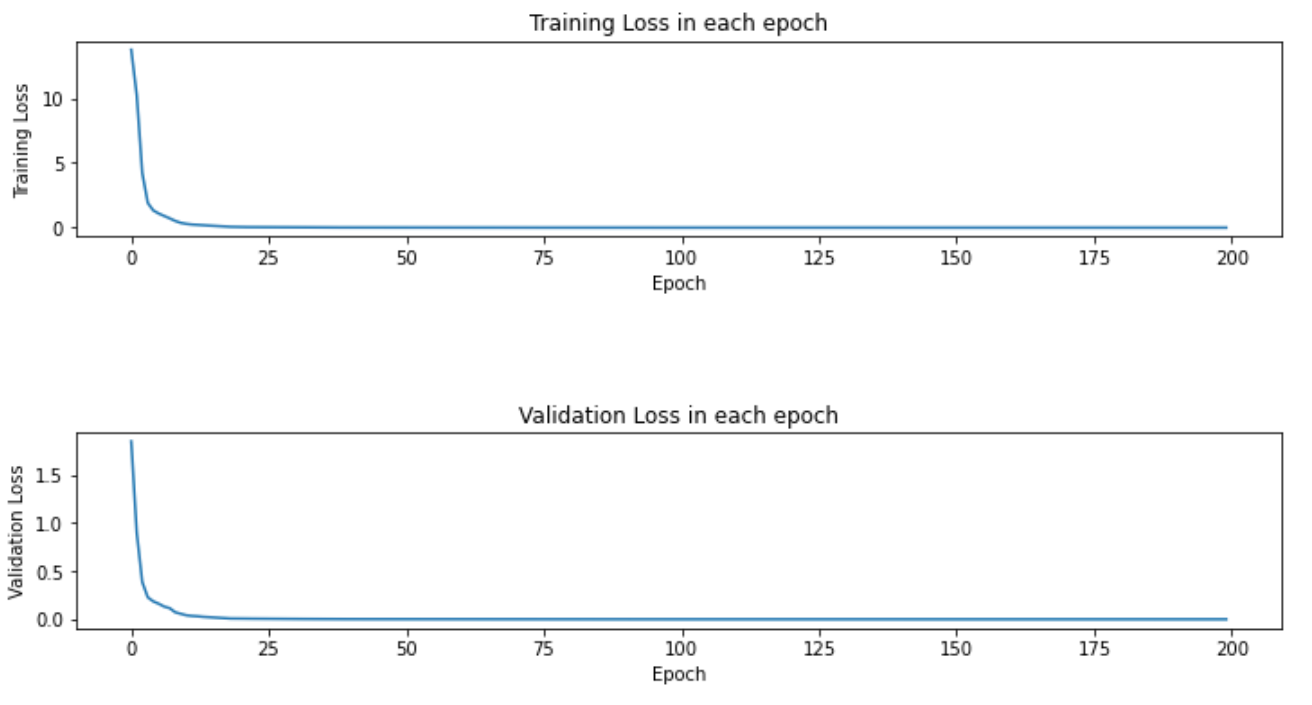
\includegraphics[scale=0.6]{figures/geoid_images/Geoid_trainingData.png}
    \label{figure:geoid_losses}
\end{figure}

\begin{figure}[H]
    \caption{Overall testing result.}
    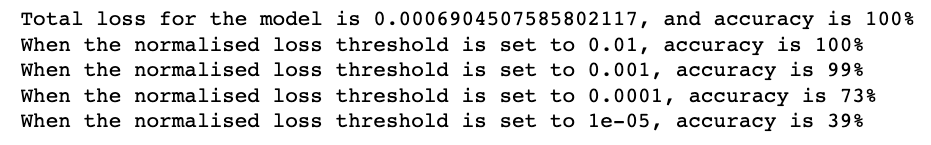
\includegraphics[scale=0.8]{figures/geoid_images/Geoid_OverallTesting.png}
    \label{figure:geoid_testing}
\end{figure}

\begin{figure}[H]
    \caption{Most accurate geoid prediction.}
    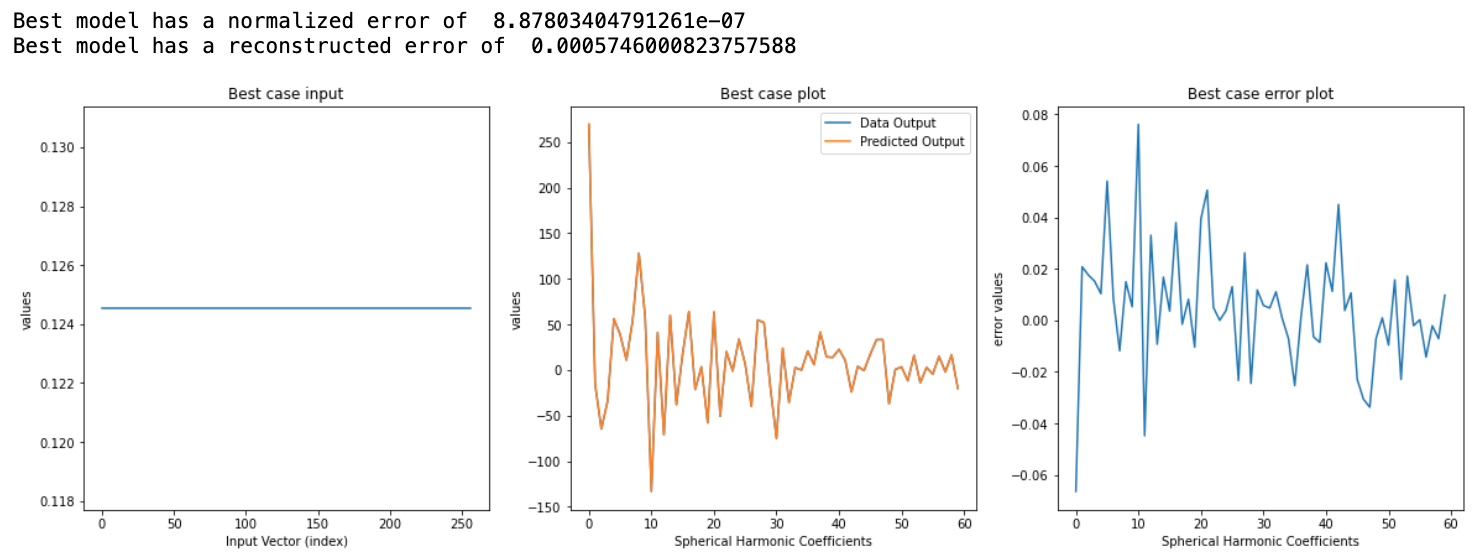
\includegraphics[scale=0.6]{figures/geoid_images/Geoid_Best.png}
    \label{figure:geoid_best}
\end{figure}

\begin{figure}[H]
    \caption{Least accurate geoid prediction.}
    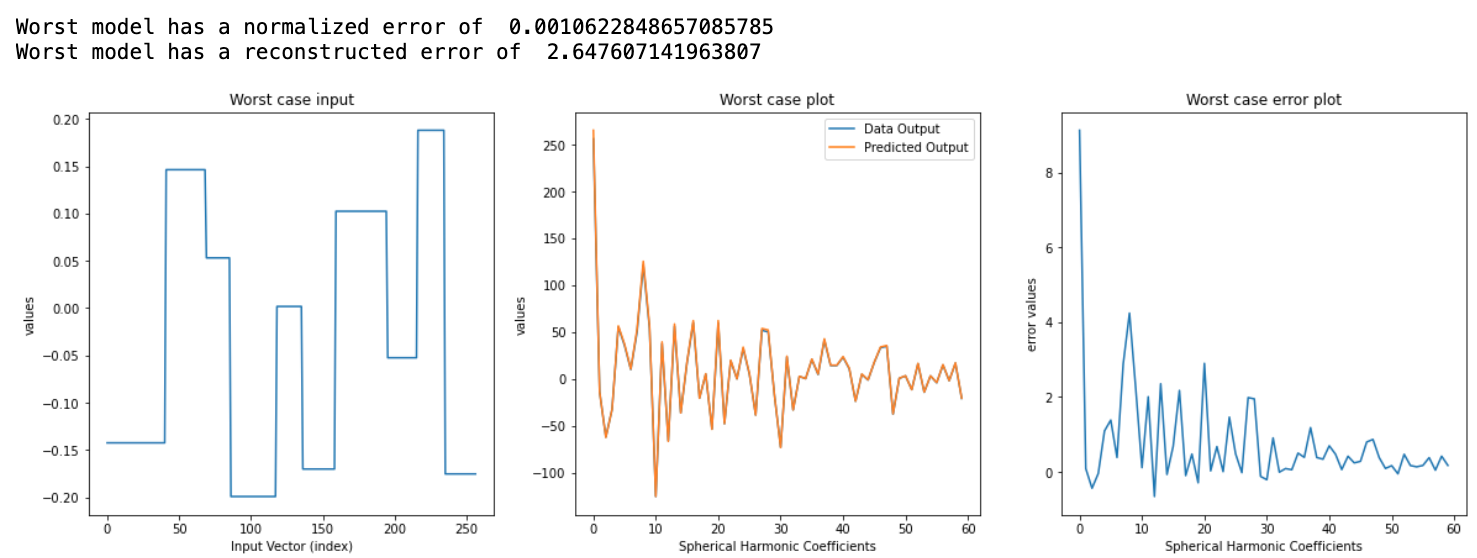
\includegraphics[scale=0.6]{figures/geoid_images/Geoid_Worst.png}
    \label{figure:geoid_worst}
\end{figure}

On average, both the normalised loss and the reconstructed loss are low and no overfitting occurs. The accuracy of the prediction is nearly 100\% when the threshold is set to be 10 times lower than the worst loss value. 

For further testings, the geoid fields constructed using the set of 60 coefficients produced by the FNN in both the best case and the worst case are visualized in Figure \ref{figure:geoid_best_visual} and Figure \ref{figure:geoid_worst_visual}, along with the fields produced by the ground truth and the error maps representing the difference between the prediction and the ground truth.

\begin{figure}[H]
    \caption{Visualization of the most accurate geoid prediction.}
    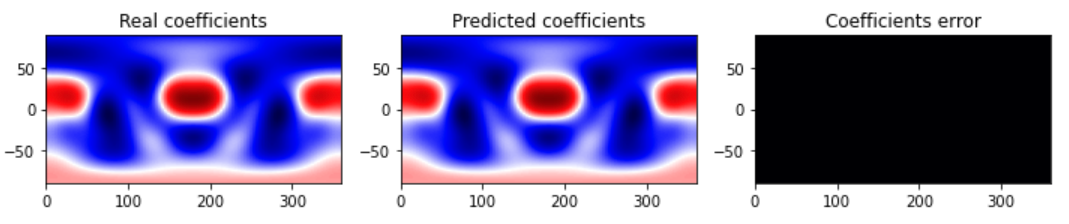
\includegraphics[scale=0.4]{figures/geoid_images/Geoid_Best_visualization.png}
    \label{figure:geoid_best_visual}
\end{figure}

\begin{figure}[H]
    \caption{Visualization of the least accurate geoid prediction.}
    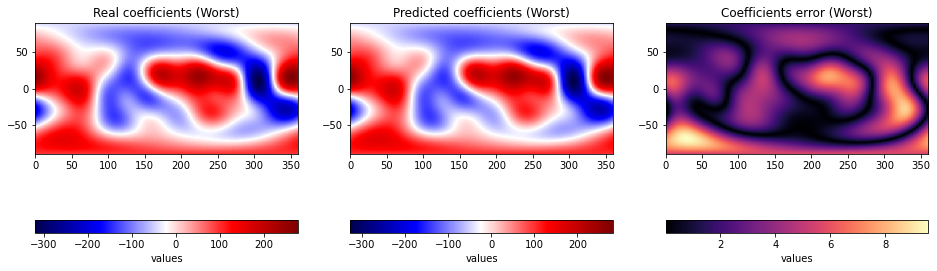
\includegraphics[scale=0.4]{figures/geoid_images/Geoid_Worst_visualization.png}
    \label{figure:geoid_worst_visual}
\end{figure}

We can observe that the result produced by the FNN is in high quality even in the worst case, where the maximum error between the real geoid field and the predicted geoid field is about 60 times less than the range of real values. The real geoid field and the predicted field also have the same patterns in both cases, meaning that FNN is able to capture the characteristic of the data in its prediction.

Overall, we constructed a systematic framework for rapidly testing different FNN architectures in a reproducible way, and we were able to create a highly accurate FNN as a surrogate forward model for the geoid problem, this could be used in further research in inverse problems involving observations of the Earths geoid.                                   % Geoid
\chapter{Mantle Convection Problem}\label{chap:evaluation}

Originally, the thermal evolution in mantle convection is modelled using the Stokes system of partial differential equations derived from the conservation equations of mass, momentum, and energy, in their simplest form of the Boussinesq approximation. Given an initial temperature, we can get a complete temperature time evolution predicted by the numerical solver, as shown below by the figure:

\begin{figure}[H]
    \caption{Typical mantle convection workflow.}
    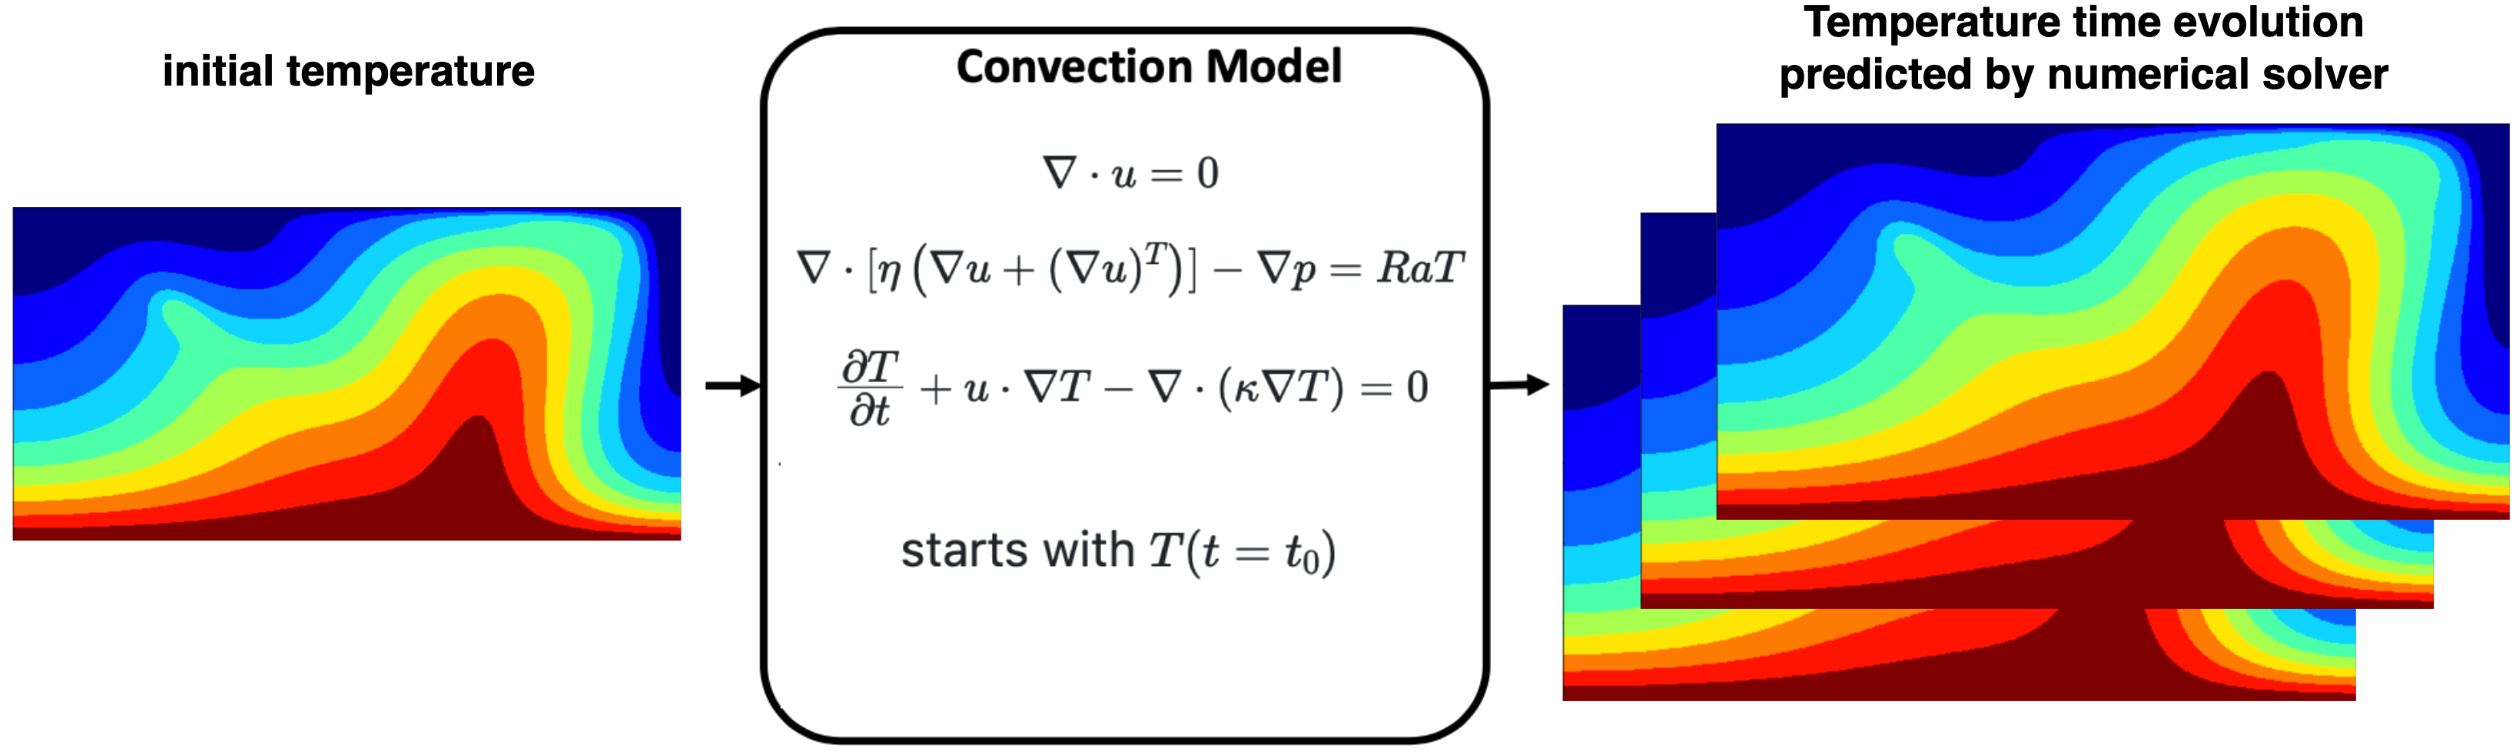
\includegraphics[scale=0.15]{figures/mantle_convection_images/Mantle_Convection_workflow.png}
\end{figure}

To explore the usage of Neural Networks as surrogate models for the original mantle convection numerical solver to significantly reduce the computational
cost, three different datasets are tested, including Limited Dataset, Larger Dataset and Interpolated Dataset. Each dataset is composed of several temperature time-series with 100 timestamps each resulting from numerical simulations with randomly sampled initial conditions (except for the Interpolated Dataset, which is created from the Larger Dataset using interpolation).

\section{Mantle Convection Simulation on Limited Dataset}

The limited dataset consists of 100 files and each of them represents one mantle convection simulation in 100 time steps generated with an initial condition with random number of points and random amplitude and coordinates of Gaussian anomalies distributed in space (a total of 10000 temperature fields). Starting from each initial condition we convect as long as there is meaningful change in the simulation (that is the temperature fields change enough after one time-step). There are 100 temperature fields with a size of $201 \times 401$ for each of the 100 timestamps in a file and the time step has to be adaptive, otherwise the whole random generation of the initial condition would be hard to implement. This adaptive timestamps lead to a problem, that is, the distance between each consecutive pairs of time steps are not the same even in the same simulation file. This could lead to some uncommon behaviors when predicting a sequence of temperature fields using the ML architecture, which will be discussed in more details in the following sections.

The following figure shows one random temperature fields in the dataset with the y-axis inverted and colored using 10-color-map (all the figures in this chapter will have their y-axis inverted and colored using 10-color-map as well, but without labels on x-axis and y-axis for better visualisation):

\begin{figure}[H]
    \caption{Temperature Field example. (For the colorbar of the upcoming figures, see this one.)}
    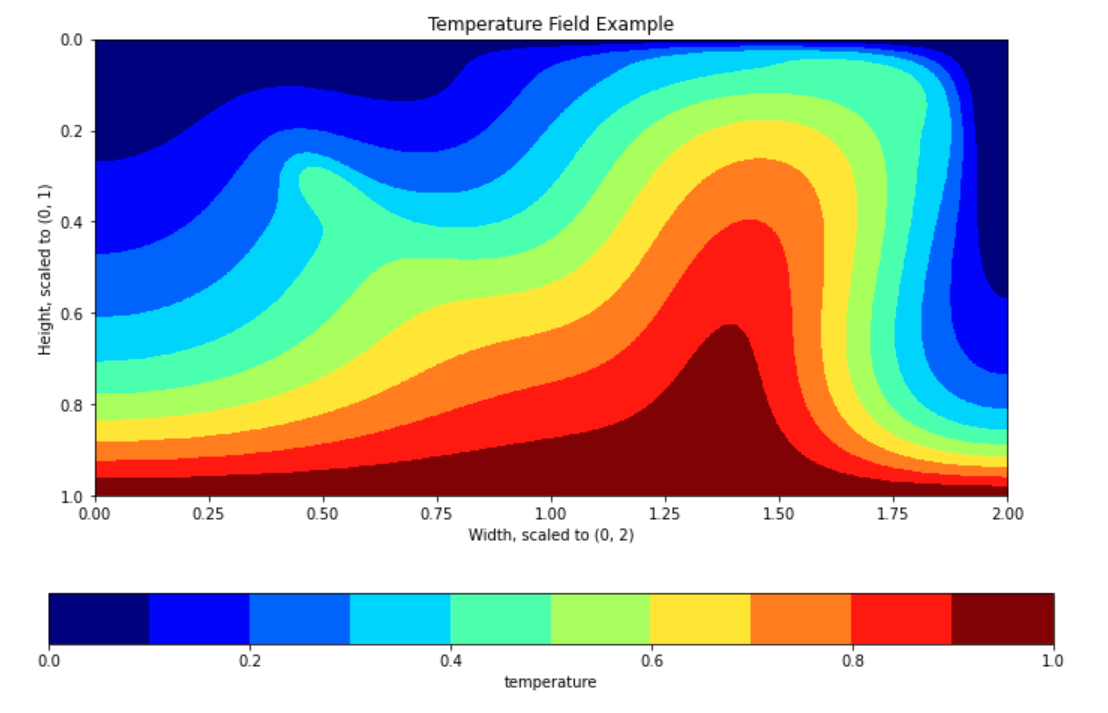
\includegraphics[scale=0.6]{figures/mantle_convection_images/temperature_field_example.png}
\end{figure}

The entire dataset is randomly divided in a ratio of 8:1:1, where 80 per cent of the dataset is used for training, 10 per cent of the data for testing and the remaining 10 per cent to perform validation and prevent overfitting. However, the way we divide them is different in implementing the ConvAE, FNN and LSTM and will be discussed in more details in the following sections.

The dataset is uploaded to Gadi, a HPC system, for storage to make the training process more efficient. 

\subsection{Compression of temperature fields}

Since applying Machine Learning (ML) algorithms directly on the original sized temperature fields can take significantly more time to train the model and could possibly lead to the risk of over-parameterization, we decided to compress the temperature fields first before feeding the data into different ML architectures.

In this study, the overall process to solve the mantle convection problem would be: 

\begin{enumerate}
  \item Train the ConvAE.
  \item Train the FNN/LSTM using the latent space representation of both input and output data. (encoder from ConvAE is used to get the the latent space representation.)
  \item Test the predicted temperature in its original size. (decoder from ConvAE is used to get the original sized temperature from the latent space representation.)
\end{enumerate}

\begin{figure}[H]
    \centering
    \caption{Workflow of ConvAE.}
    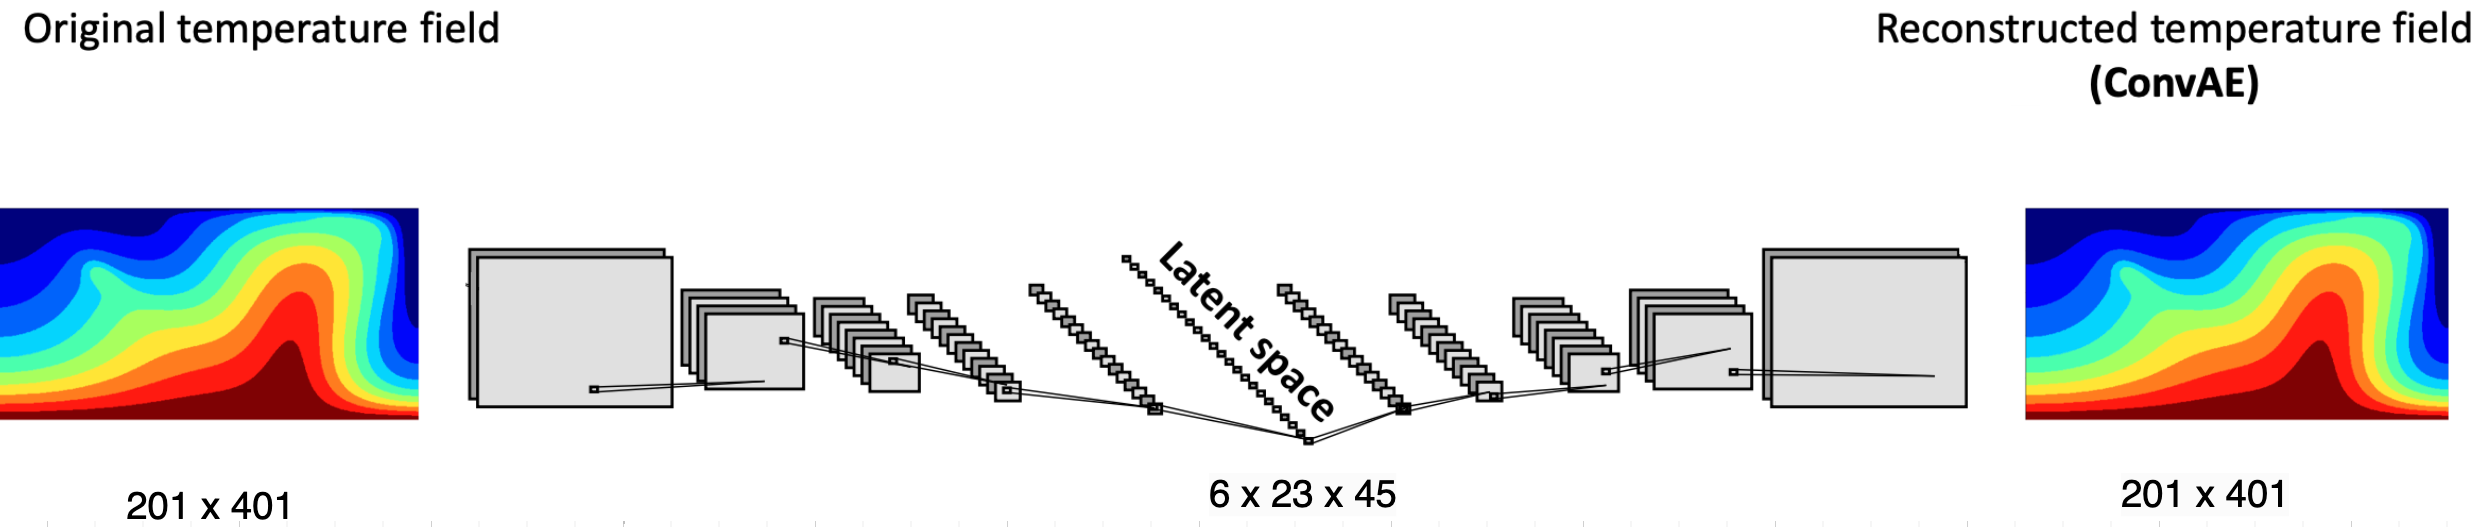
\includegraphics[scale=0.3]{figures/mantle_convection_images/ConvAE_workflow.png}
\end{figure}

\begin{figure}[H]
    \centering
    \caption{Workflow of FNN.}
    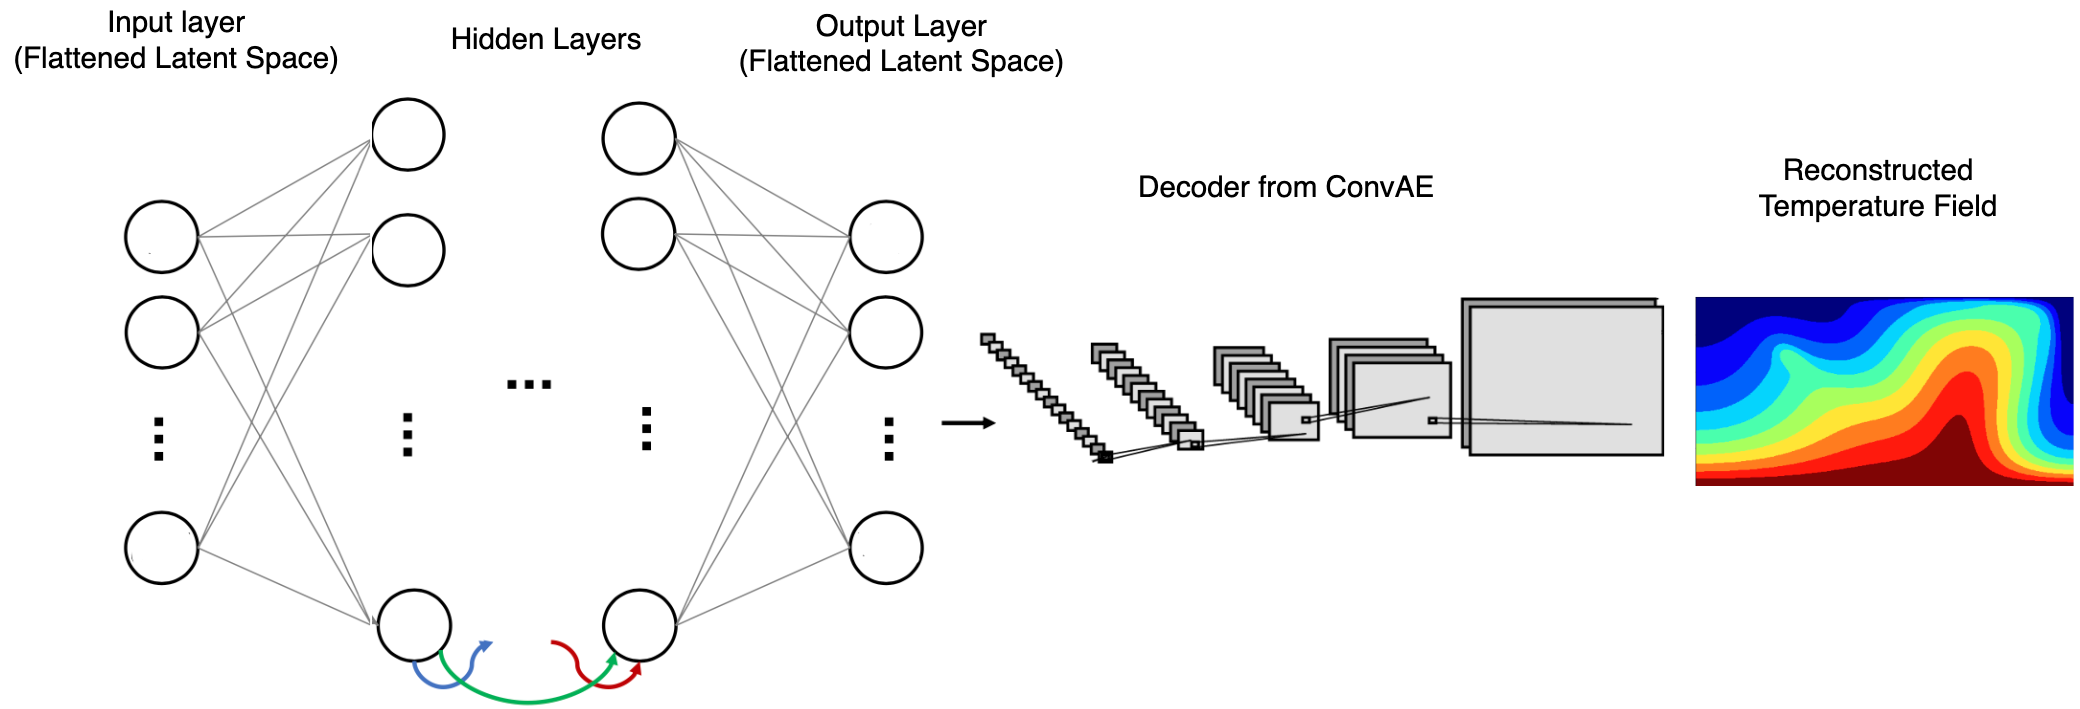
\includegraphics[scale=0.4]{figures/mantle_convection_images/FNN_workflow.png}
\end{figure}

\begin{figure}[H]
    \centering
    \caption{Simple Workflow of LSTM, where Tn is a temperature field in its latent space representation. Here we input the first 50 temperature fields (after compressed and flattened) from a simulation into the LSTM and hopefully LSTM would predict the rest 50 temperature fields of the same simulation (also compressed and flattened).(Source of the left figure: StackOverflow.)}
    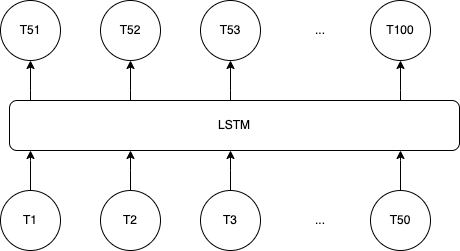
\includegraphics[scale=0.6]{figures/mantle_convection_images/LSTM_workflow.png}
\end{figure}

The complete 10000 temperature fields are randomly shuffled and divided in a ratio of 80\%, 10\%, 10\% for training, testing and validation where each piece of data consists only one temperature field (fed as both the input and output during training and testing). Given the size of the training set, ConvAE is fed with a batch size of 16 temperature fields during the training to perform Mini-Batch Gradient Descent.

We find that ConvAE with a latent space size of $6 \times 23 \times 45$ offers an excellent compression factor of 13, while being able to reconstruct the temperature fields in its original size with the lowest data loss on the test set.

The architecture of the ConvAE in this case consists of two convolutional layers for the encoder and two transpose convolutional layers for the decoder. Both of these four layers have the size of the filter as $5 \times 5$ and a stride of $3 \times 3$. Tanh() is used as the activation function to introduce non-linearity between each layers (except for the last layer in the decoder) and mean square error (MSE) is used as the loss function. The model is trained for 1000 epochs on Gadi.

In the following figures, we present some detailed test results from this ConvAE:

\begin{figure}[H]
    \caption{Training loss and Validation loss of ConvAE trained with Limited Dataset.}
    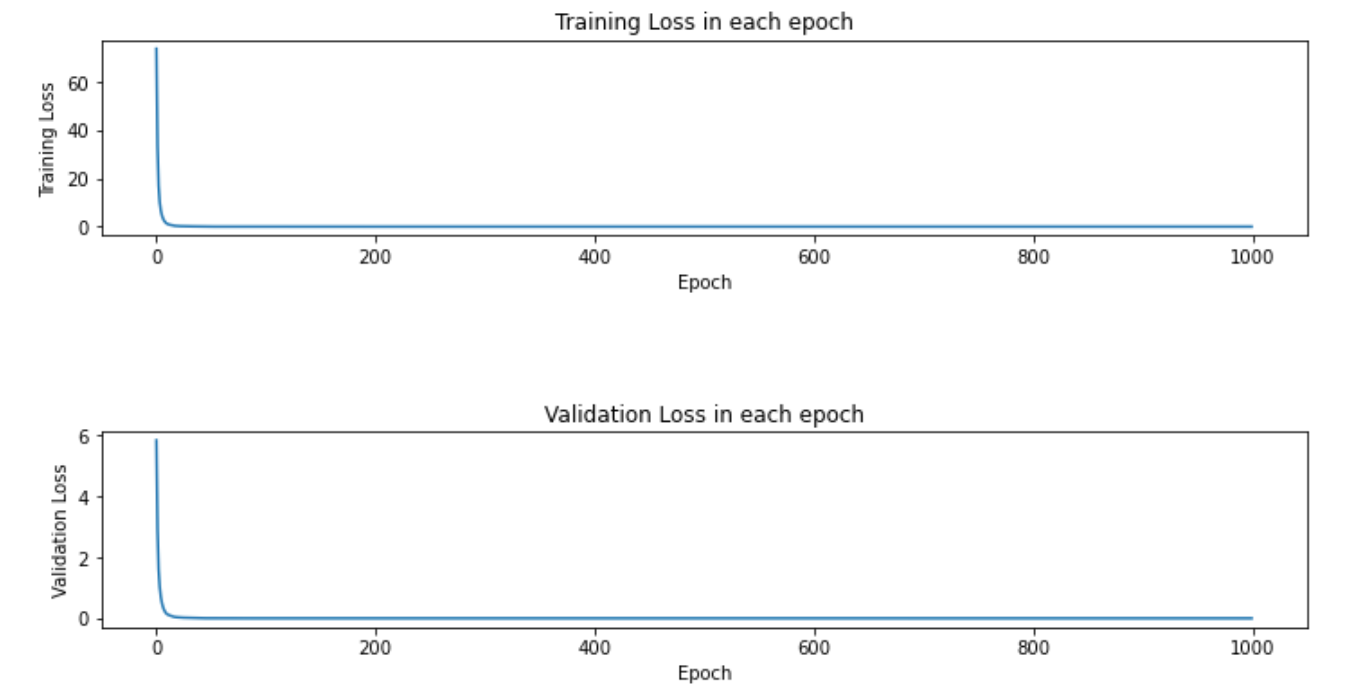
\includegraphics[scale=0.6]{figures/mantle_convection_images/limited_dataset/ConvAE_trainingData.png}
\end{figure}

\begin{figure}[H]
    \caption{Overall testing result of ConvAE trained with Limited Dataset.}
    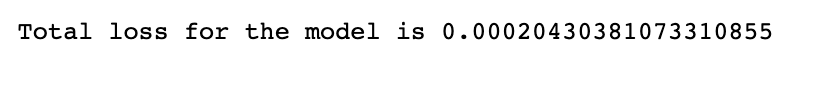
\includegraphics[scale=0.8]{figures/mantle_convection_images/limited_dataset/ConvAE_OverallTesting.png}
\end{figure}

\begin{figure}[H]
\centering
\begin{subfigure}{0.45\textwidth}
    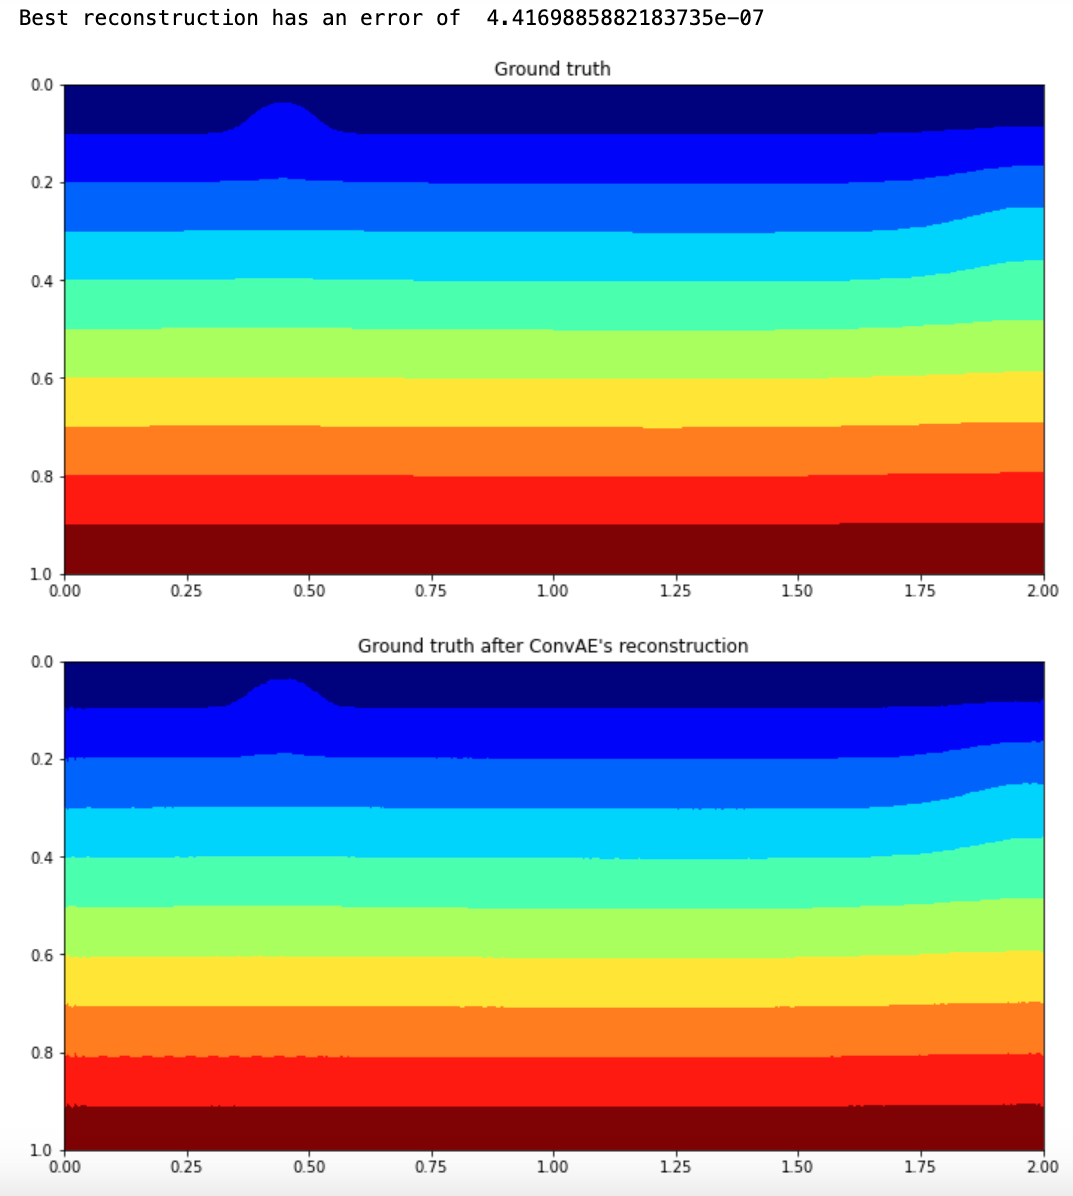
\includegraphics[width=\textwidth]{figures/mantle_convection_images/limited_dataset/ConvAE_Best.png}
    \caption{Best Case of ConvAE trained with Limited Dataset.}
\end{subfigure}
\hfill
\begin{subfigure}{0.45\textwidth}
    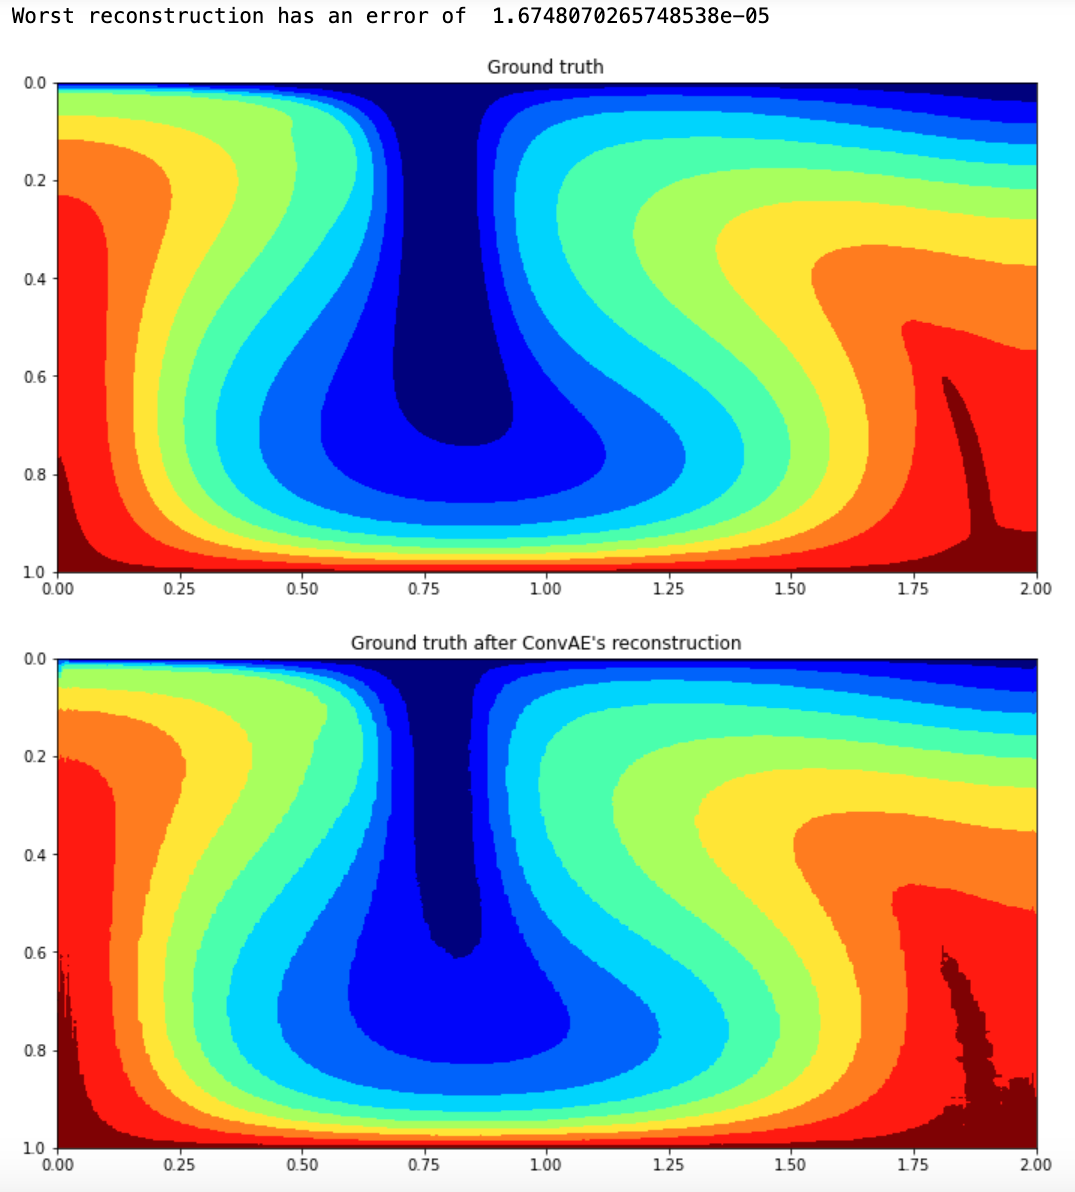
\includegraphics[width=\textwidth]{figures/mantle_convection_images/limited_dataset/ConvAE_Worst.png}
    \caption{Worst Case of ConvAE trained with Limited Dataset.}
\end{subfigure}
        
\caption{Best case and worst case using ConvAE.}
\end{figure}


On average, the reconstruction loss are low and no overfitting occurs. However, we can observe that the ConvAE does not reconstructe the thin feature in the bottom right corner of the worst case. This could imply that the ConvAE works best for "smooth" input hence others with small scale length features will generally perform worse.

We also applied some POD (Proper Orthogonal Decomposition) analysis to the compressed-decompressed fields with contrast to the original temperature fields and the result is great as well, the figure to this analysis will be presented in the following sections as contrast to the POD analysis of the prediction model (FNN or LSTM) 


\subsection{Fully Connected Neural Network for Prediction}

We now move on to predict the latent space representation and our first candidate is the feedforward fully connected neural network (FNN). The FNN in this study uses each adjacent pair of temperature fields (e.g. $i$th and ($i+1$)th fields) as one training set, takes one temperature fields as the input and output the temperature fields at the next time step. Therefore, the dataset is reconstructed into 9900 pairs of temperature fields with consecutive timestamps. These pairs are randomly shuffled and divided in a ratio of 80\%, 10\%, 10\% for training, testing and validation where each piece of data consists two temperature field having consecutive timestamps.

Before the latent space representation is fed as the input of FNN, it is flattened into one dimension. The prediction of FNN in this case is then resized from a one dimensional vector ($1 \times 6210$) to the shape of the latent space ($6 \times 23 \times 45$) for the convenience of further testing.

The learnable parameters of FNN are optimized using small mini-batches of 16 pairs of consecutive temperature fields and Adam as the optimizer, where the loss function is defined as the mean square error (MSE) between the prediction of FNN and the actual output (both in the shape of latent space representation, which is $6 \times 23 \times 45$).

After testing with FNNs that have different number of hidden layers and neurons per hidden layer, we found that architectures with a total number 3 hidden layers seemed to perform the best. (We also test some deeper architectures with 4-5 hidden layers. However, there is no significant reduction in the loss value)

In the following figures, we present results from a FNN with 3 hidden layers with 3105, 1035 and 3105 neurons, Tanh() as activation function, and trained for 1000 epochs.

\begin{figure}[H]
    \caption{Training loss and Validation loss of FNN trained with Limited Dataset.}
    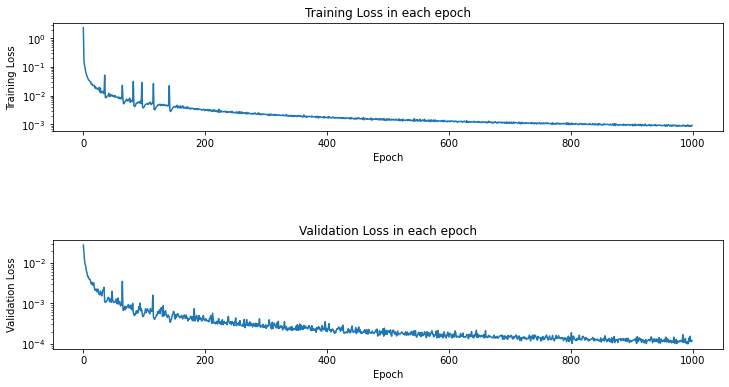
\includegraphics[scale=0.6]{figures/mantle_convection_images/limited_dataset/FNN_trainingData.png}
\end{figure}

\begin{figure}[H]
    \caption{Overall testing result of FNN trained with Limited Dataset.}
    
\includegraphics[scale=0.8]{figures/mantle_convection_images/limited_dataset/FNN_OverallTesting.png}
\end{figure}

\begin{figure}[H]
    \caption{Best case original output, original output after ConvAE's compression-decompression, and predicted output of FNN trained with Limited Dataset.}
    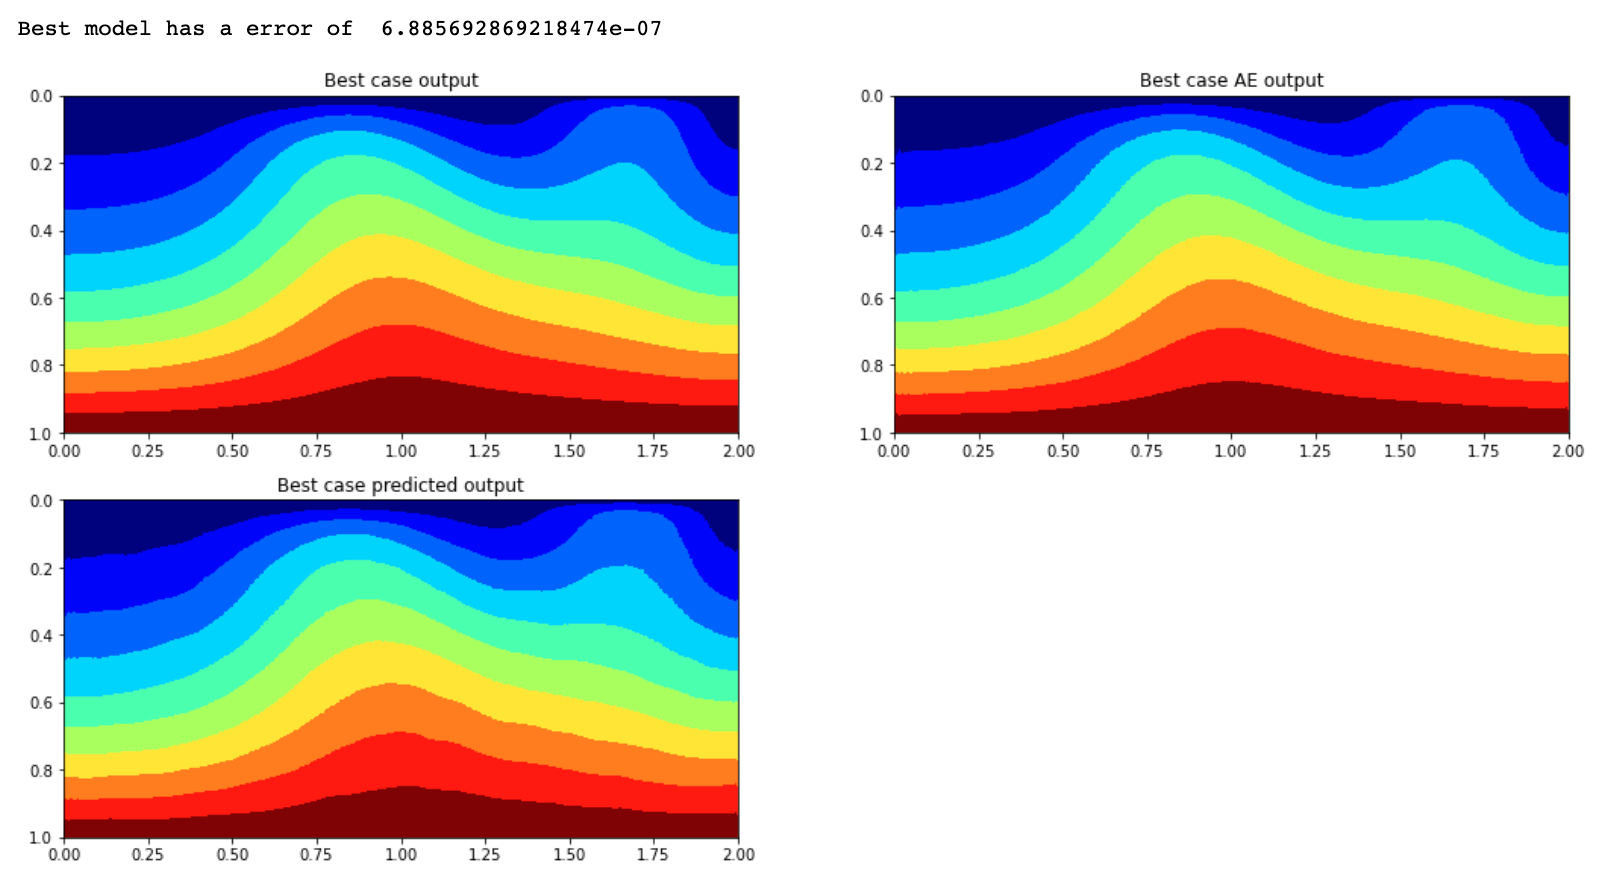
\includegraphics[scale=0.5]{figures/mantle_convection_images/limited_dataset/FNN_Best.png}
\end{figure}

\begin{figure}[H]
    \caption{Worst case original output, original output after ConvAE's compression-decompression, and predicted output of FNN trained with Limited Dataset.}
    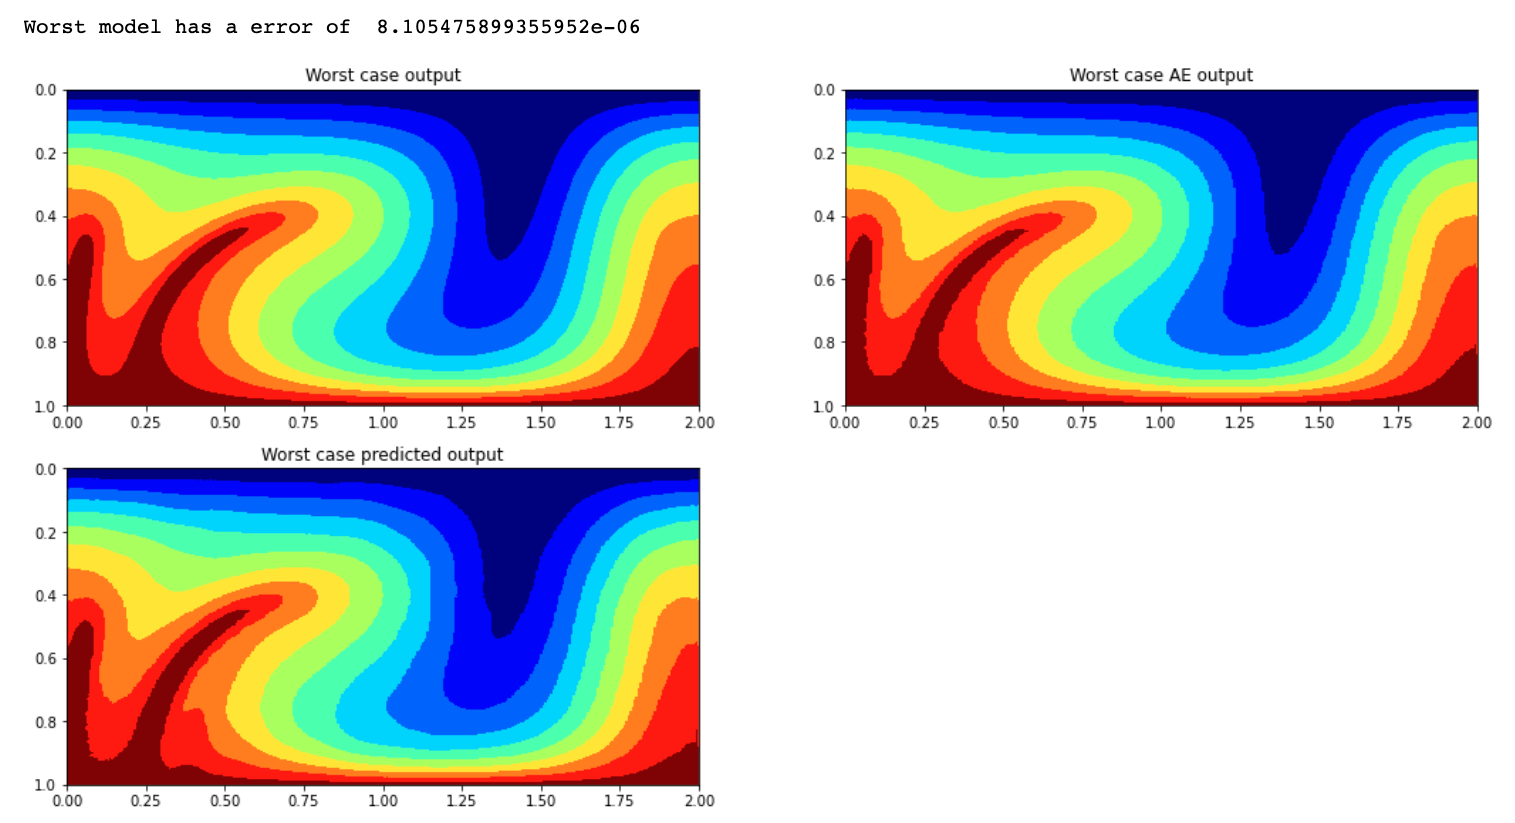
\includegraphics[scale=0.5]{figures/mantle_convection_images/limited_dataset/FNN_Worst.png}
\end{figure}

On average, the loss values are low and no overfitting occurs. The prediction for the temperature field at the next timestamp is able to capture the main features precisely with some small information loss, which is partially due to information loss caused by the compression-decompression process of ConvAE.

To further evaluate the performance of FNN in predicting a complete time series, two methods are tested on all 100 simulations one by one: 

\begin{enumerate}
  \item "One-for-All" (also referred as "Output-as-input Prediction"): Only take the first temperature field in the file as the input and use a prediction-as-input loop to get the rest of the 99 temperature fields. (use $T1$ from dataset $\rightarrow$ get predicted $T2$ $\rightarrow$ use predicted $T2$ $\rightarrow$ get predicted $T3$ $\rightarrow$ ...)
  \item "One-for-One" (also referred as "Single Prediction"): Constantly feed a temperature field from the original dataset and get the temperature field at the next time step as usual. (use $T1$ from dataset $\rightarrow$ get predicted $T2$ $\rightarrow$ use $T2$ from dataset $\rightarrow$ get predicted $T3$ $\rightarrow$ ...)
\end{enumerate}

In this case, the first method can reduce the computation complexity of the mantle convection problem more effectively than the second method, since we only need one initial input data and the model can generate the rest of the temperature field sequence. Therefore, the following best case and worst case will be evaluated using the data loss of the first method.

To better visualize the prediction result of the above two methods, two animations representing the best case and the worst case (evaluated based on the sum of MSE for each prediction using the first method) in the format of GIF files are generated. From top to bottom, the first picture represents the actual output from the dataset, the second one represents the prediction result using the first method, and the last one represents the prediction result using the second method.

The following figures show 10\% of the sprite sheets converted from the original GIFs (every 10th frame) for the convenience of reading:

\begin{figure}[H]
    \centering
    \caption{Best case animation sheet of FNN trained with Limited Dataset (Link to this GIF: \url{https://drive.google.com/file/d/1Hmb4UlevBHMRw0jDScTwUzDFPbYNubKO/view?usp=sharing})}
    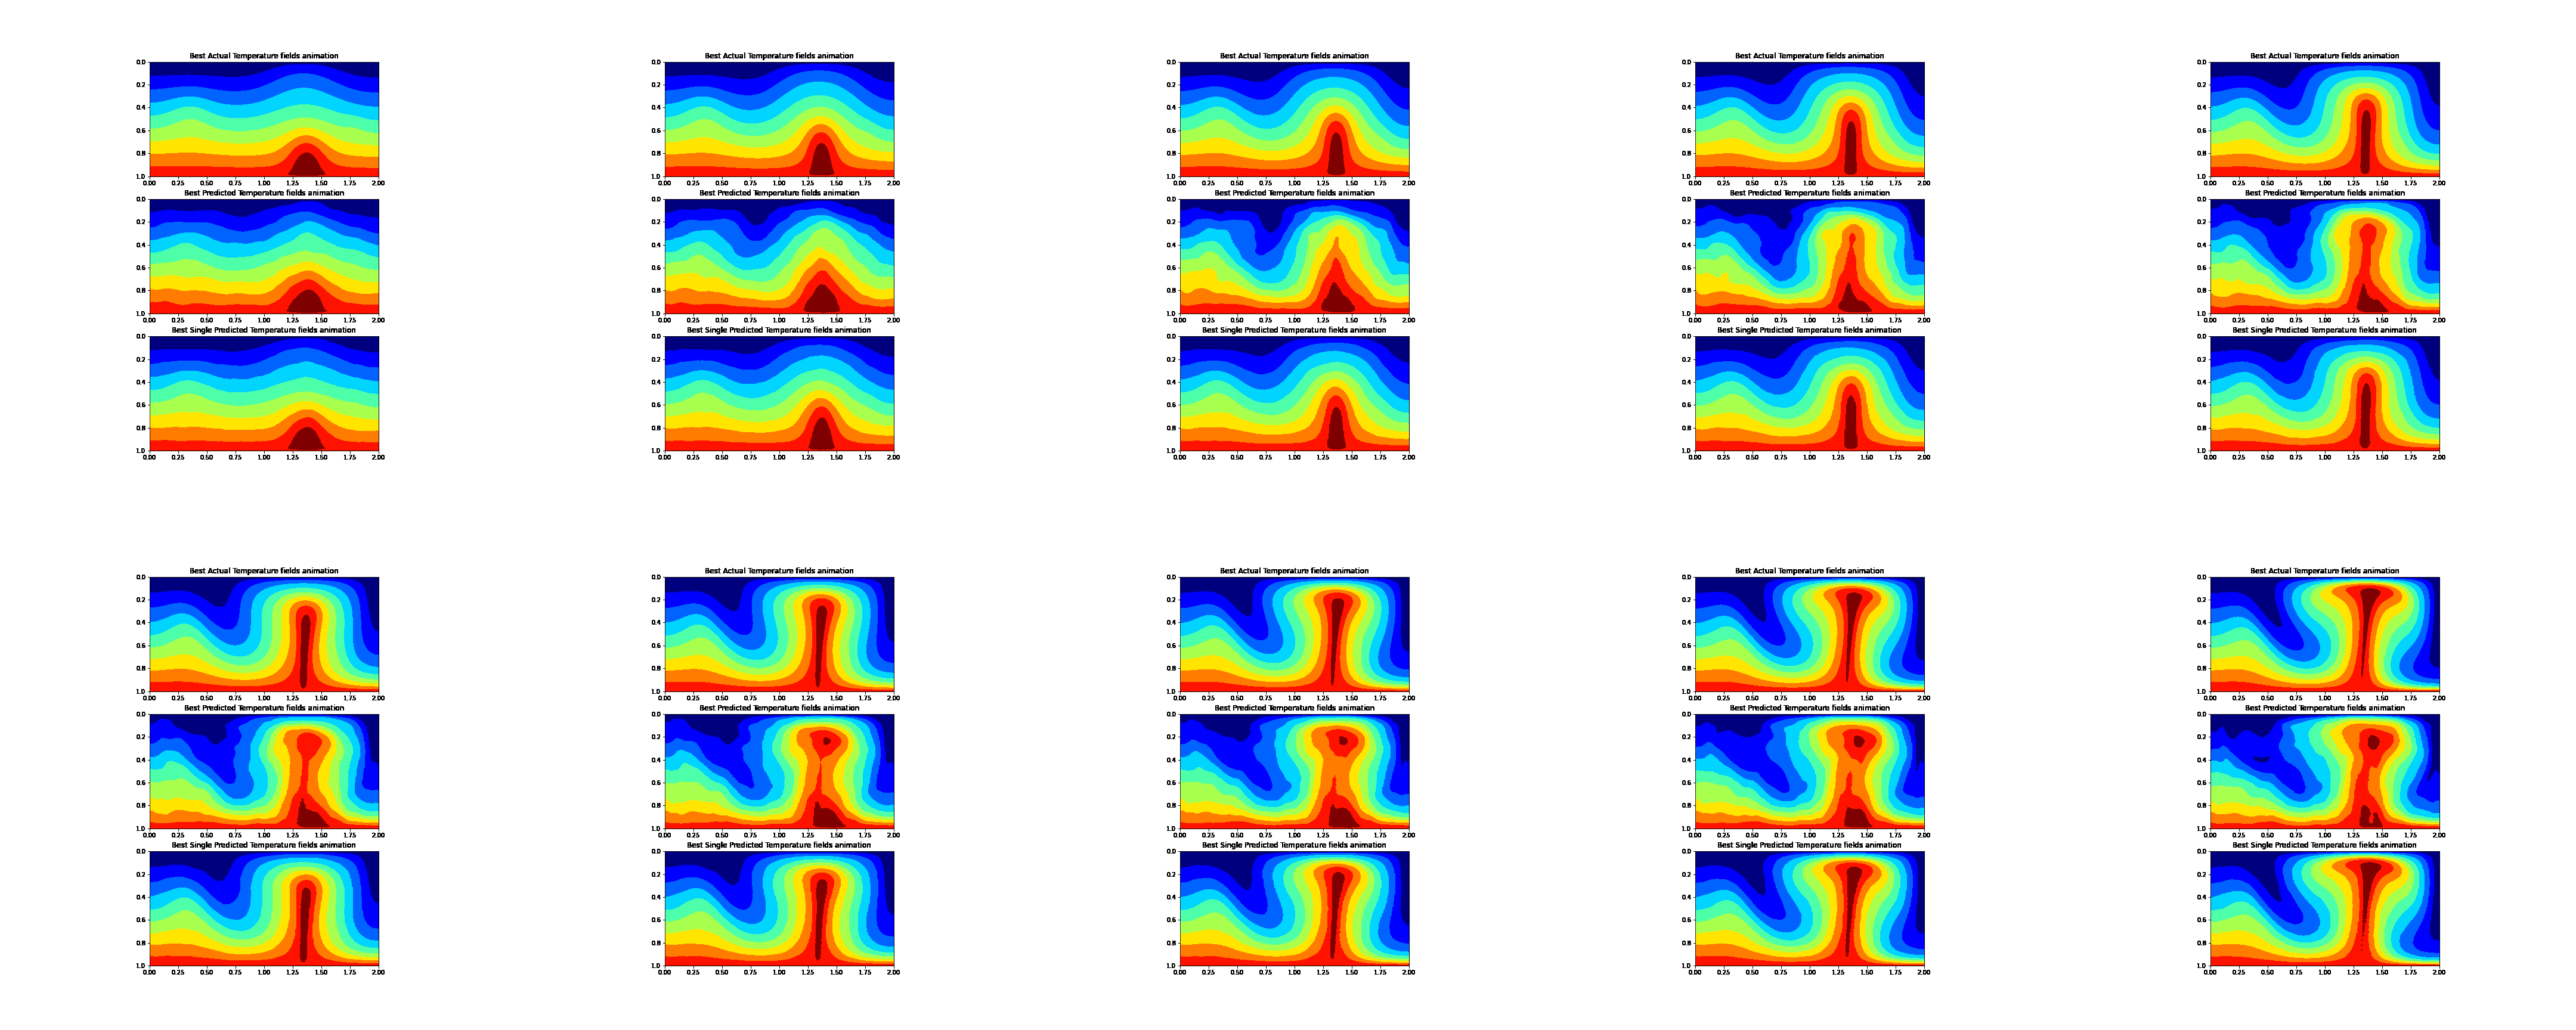
\includegraphics[scale=0.10]{figures/mantle_convection_images/limited_dataset/FNN_Best_GIF_sheet.png}
\end{figure}

\begin{figure}[H]
    \centering
    \caption{Worst case animation sheet of FNN trained with Limited Dataset (Link to this GIF: 
    \url{https://drive.google.com/file/d/11jRFxq-XuIUvTk74OuxswDn3u031k_q7/view?usp=sharing})}
    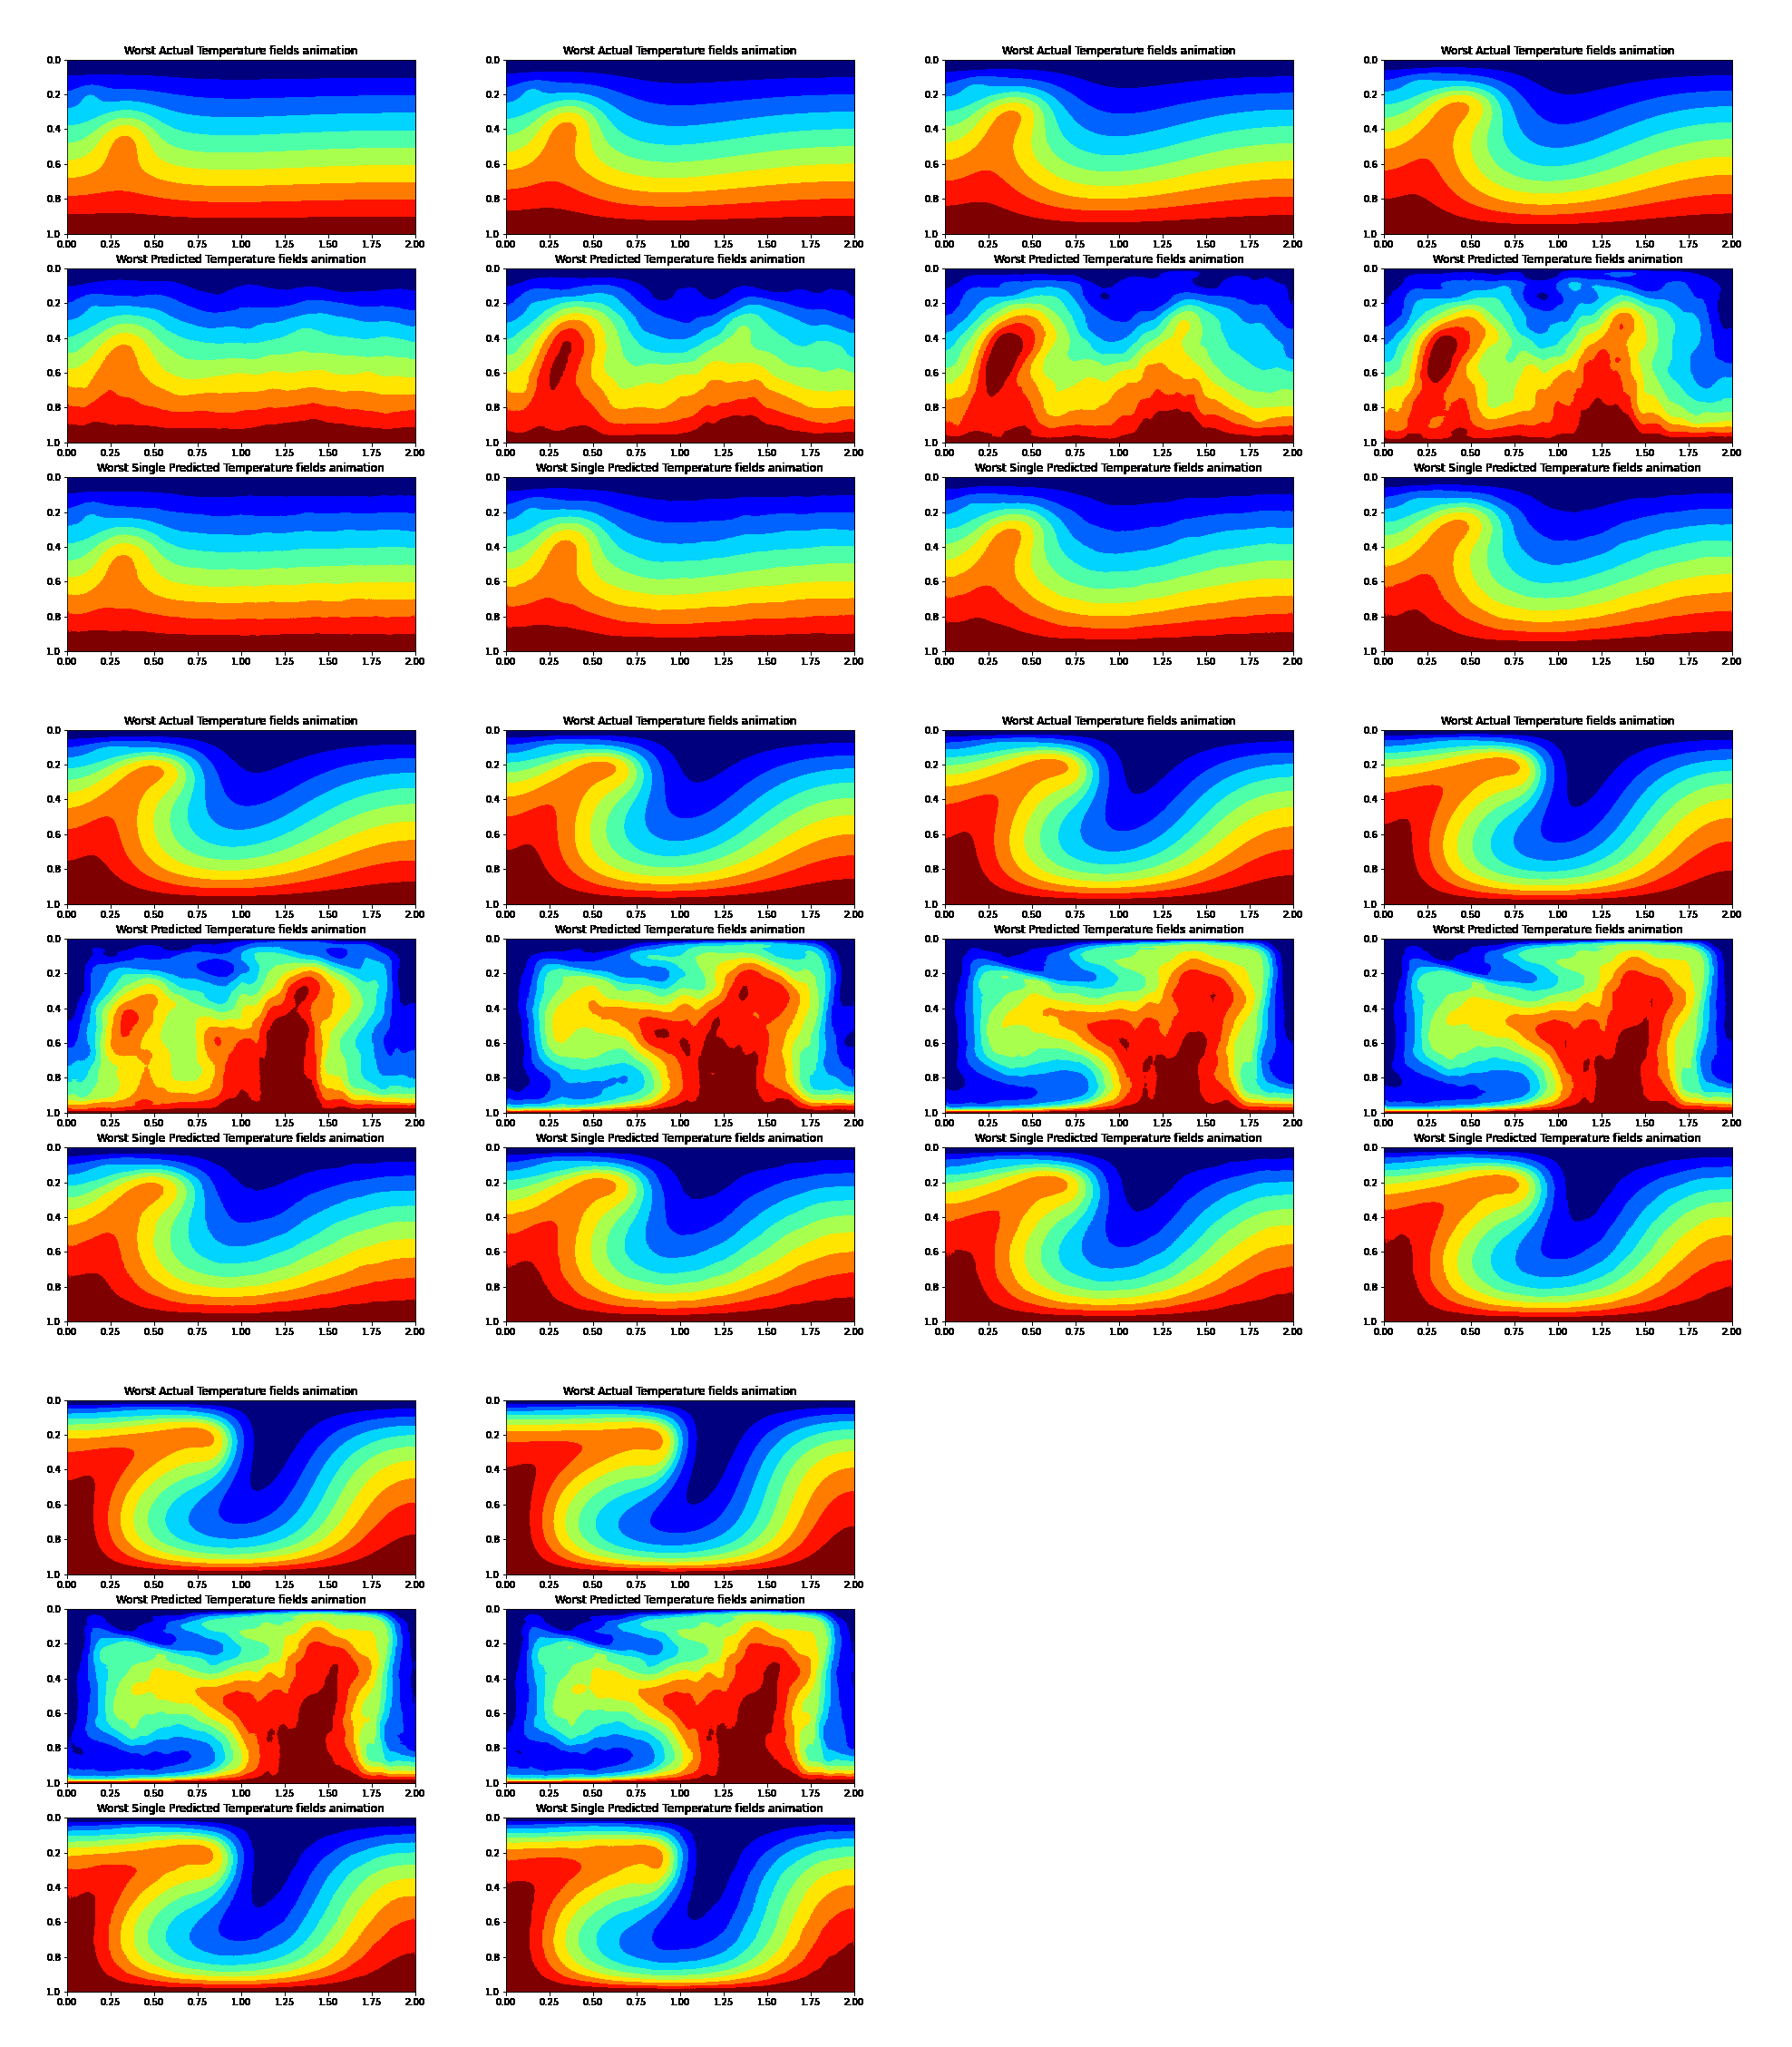
\includegraphics[scale=0.10]{figures/mantle_convection_images/limited_dataset/FNN_Worst_GIF_sheet.png}
\end{figure}

To further evaluate the performance of these two methods, we applied a technique called Proper Orthogonal Decomposition (POD) to the set of predictions generated by these two methods in both the best case and the worst case, along with the original time series and the compressed-decompressed version generated by ConvAE serve as contrast.

POD is mainly used to decompose a physical field (e.g. temperature field) depending on the different variables that influence its physical behaviors and it is similar to Principle Component Analysis (PCA) since it refers to eigenvalues of a physical field.\citep{10.1146_annurev.fl.25.010193.002543} Following \citep{10.1515_9783110671490-007}, the Singular Value Decomposition (SVD) of a simulation matrix $X$ (spatial points × time-steps, in this case it's $201 \times 401 \times 100$) is computed as:

\begin{equation}
X = U\Sigma V
\end{equation}

where the diagonal of $\Sigma$ contains the eigenvalues (POD coefficient) for this simulation.

The following figures show the POD result in the best case and the worst case:

\begin{figure}[H]
    \caption{Best case POD of FNN trained with Limited Dataset.}
    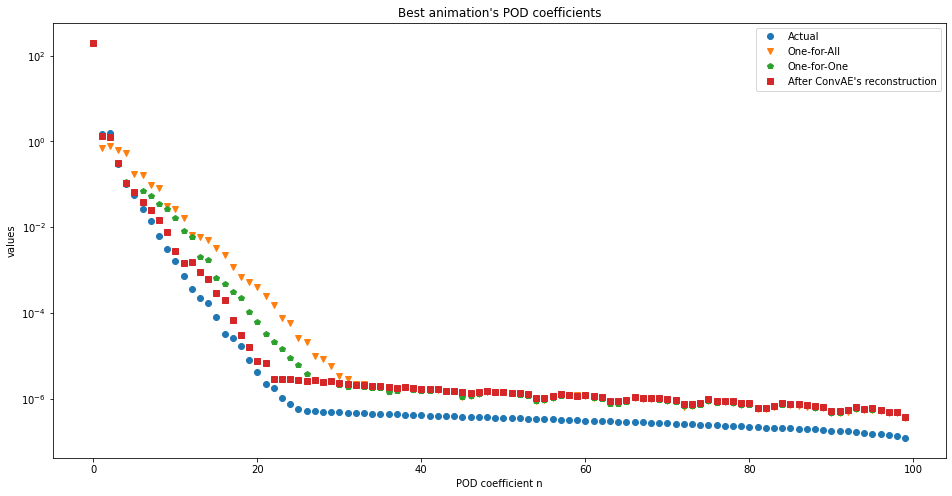
\includegraphics[scale=0.5]{figures/mantle_convection_images/limited_dataset/FNN_Best_POD.png}
\end{figure}

\begin{figure}[H]
    \caption{Worst case POD of FNN trained with Limited Dataset.}
    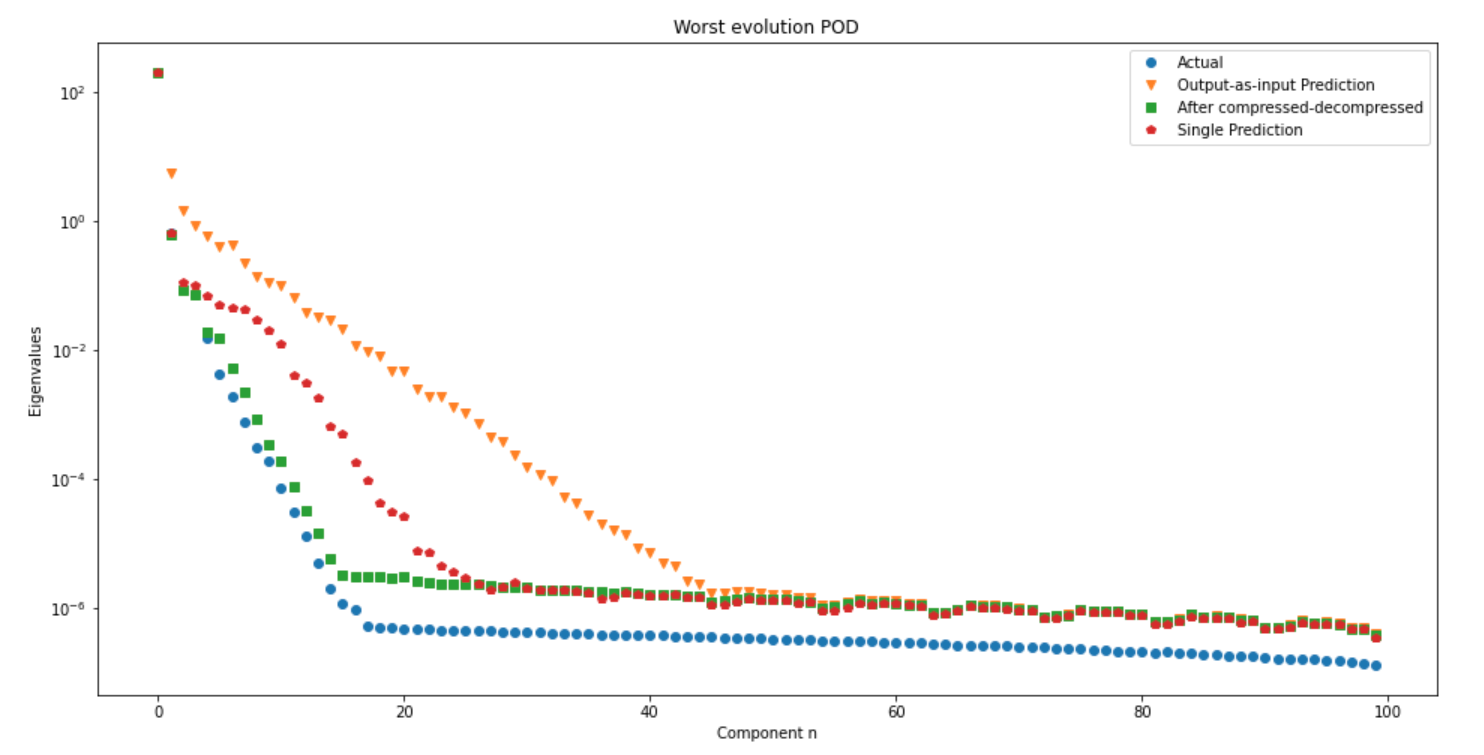
\includegraphics[scale=0.5]{figures/mantle_convection_images/limited_dataset/FNN_Worst_POD.png}
\end{figure}

As seen in the animations and the POD results, the first method (output-as-input prediction) fails to capture the trend of the temperature fields simulations in the worst case and the result prediction is completely different to the actual simulations. This is because the information loss from the ConvAE and FNN in each prediction-as-input loop accumulates, leading to poor result after 99 iterations. In the mean time, the prediction result for the second method mostly matches with the actual output in both cases, which is consistent to our theory that the it is the first method itself leads to the huge information loss.

Also, the predicted GIFs in this case are either moving faster or slower than the actual simulation. This is probably due to the varying distance between time steps in the simulation. In this case, the model will try to predict the temperature field at the next time step by averaging out the distance between each time step, thus making the predicted simulations either too fast or too slow.

To explore if we can generate a sequence of temperature fields with less information loss, we try to use LSTM to predict the latent space representation instead.


\subsection{Long Short-Term Memory (LSTM) for Prediction}

We now move on to predict a sequence of latent space representation using LSTM. The LSTM in this study uses the first 50 temperature fields as a sequence in each file as one training set, takes a sequence of 50 temperature fields as the input and output the rest 50 temperature fields at the next time steps.

This 50:50 of input-output length is determined by PyTorch's technical limitation on LSTM, where the input length and the output length should be the same for the LSTM to functionally work. A ratio of less input length and more output length (20:80) had been considered, but this requires the input sequence to be replicated into 4 times the size to match with PyTorch's requirement, which could lead to worse prediction result compared with the 50:50 ratio.

Therefore, the files in the dataset are randomly shuffled and divided in a ratio of 80\%, 10\%, 10\% for training, testing and validation where each piece of data is a complete file to be divided in half as input and output.

Again, before a sequence of latent space representation is fed as the input of LSTM, it is flattened into two dimension ($50 \times 6210$). The prediction of LSTM in this case is then resized from $50 \times 6210$ to $50 \times 6 \times 23 \times 45$ for the convenience of further testing.

The learnable parameters of LSTM are optimized using small mini-batches (only 1 batch in this case since we have merely 80 training samples) and Adam as the optimizer, where the loss function is defined as the MSE between the prediction of LSTM and the actual output (both in the shape of a sequence of latent space representation, which is $50 \times 6 \times 23 \times 45$).

After testing with LSTMs that have different architectures, we found that architectures with a total number of 2 consecutive LSTM layers perform the best. (We also test some deeper architectures with 4-6 LSTM. However, there is no significant reduction in the loss value)

In the following figures, we present results from an architecture with 2 LSTM layers (first one input size is 6210, hidden size is 3105; second one input size is 3105, hidden size is 6210. Both of them only have one layer, no internal stacking), and trained for 200 epochs.

\begin{figure}[H]
    \caption{Training loss and Validation loss of LSTM trained with Limited Dataset.}
    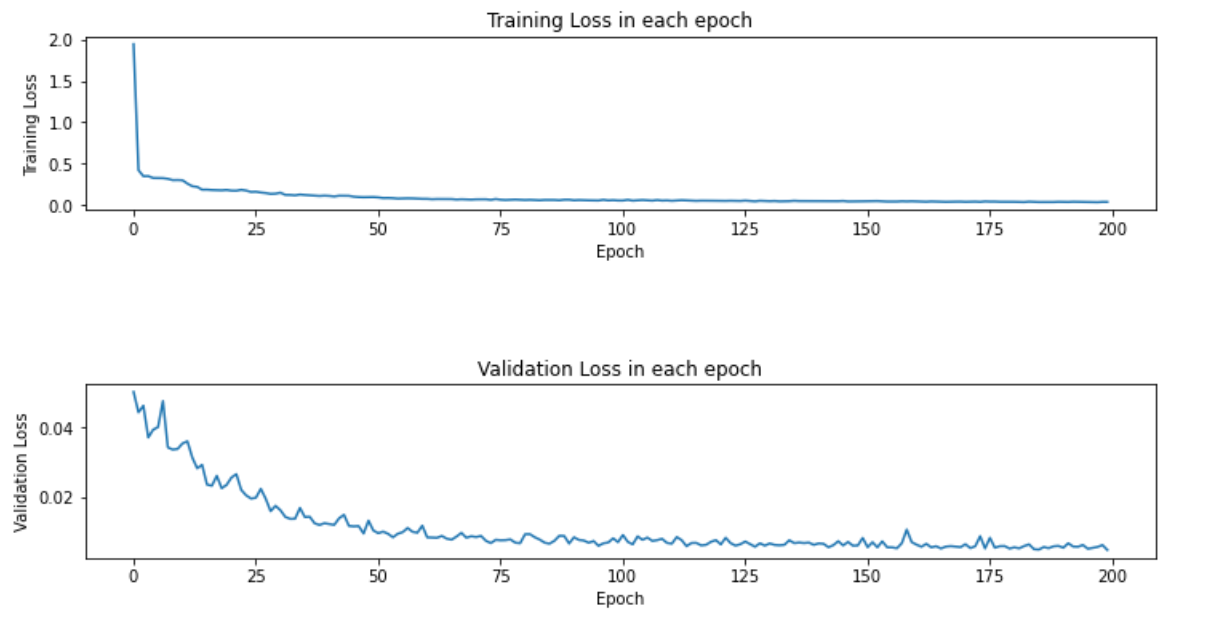
\includegraphics[scale=0.6]{figures/mantle_convection_images/limited_dataset/LSTM_trainingData.png}
\end{figure}

\begin{figure}[H]
    \caption{Overall testing result of LSTM trained with Limited Dataset.}
    
\includegraphics[scale=0.8]{figures/mantle_convection_images/limited_dataset/LSTM_OverallTesting.png}
\end{figure}

\begin{figure}[H]
    \caption{Best case original output, original output after ConvAE's compression-decompression, and predicted output of LSTM trained with Limited Dataset.}
    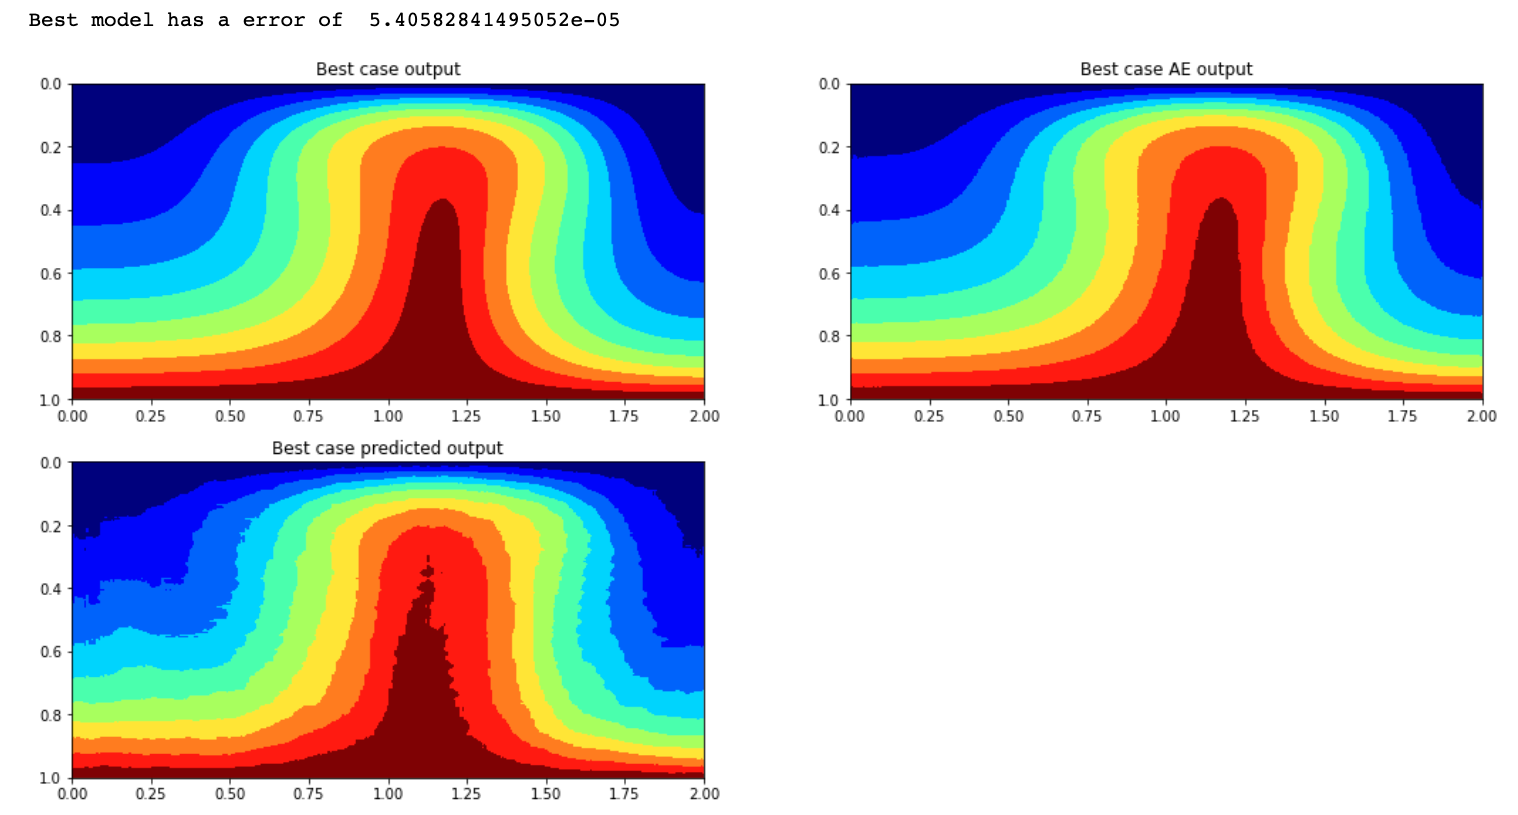
\includegraphics[scale=0.5]{figures/mantle_convection_images/limited_dataset/LSTM_Best.png}
\end{figure}

\begin{figure}[H]
    \caption{Worst case original output, original output after ConvAE's compression-decompression, and predicted output of LSTM trained with Limited Dataset.}
    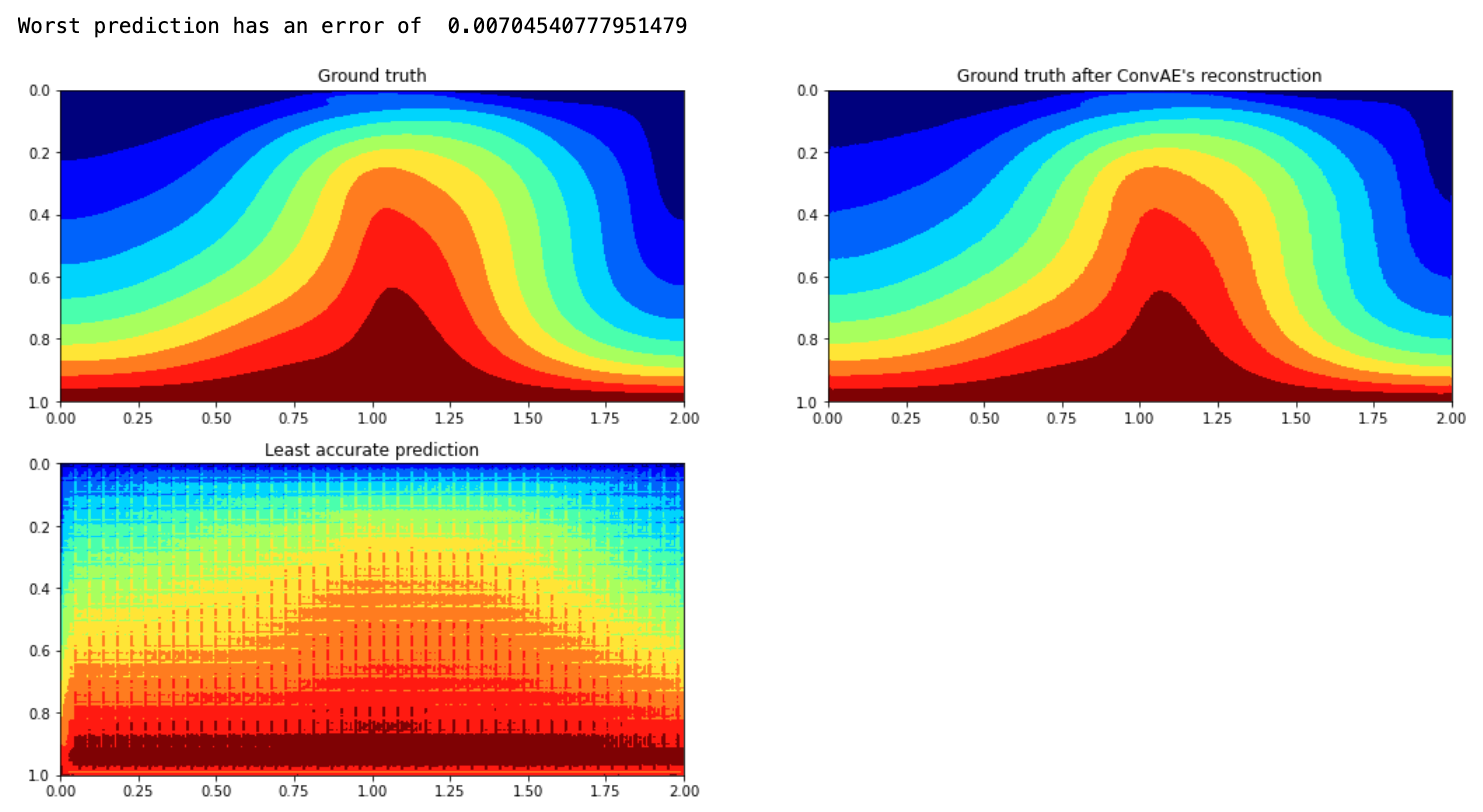
\includegraphics[scale=0.5]{figures/mantle_convection_images/limited_dataset/LSTM_Worst.png}
\end{figure}

On average, the loss values are higher than the FNN and no overfitting occurs. The prediction is able to capture the main features precisely with some small information loss in the best case, but fails to do so in the worst case. This is caused by the internal structure of LSTM since the worst case is the first temperature field in the output sequence.

To better visualize the prediction result of LSTM on a 50:50 input length to output length ratio, two animations representing the best case and the worst case (evaluated based on the sum of MSE for each predicted temperature in the output sequence) in the format of GIF files are generated. From top to bottom, the first picture represents the actual output from the dataset and the second one represents the prediction result.

The following figures show 20\% of the sprite sheets converted from the original GIFs (Every 5th frame) for the convenience of reading:

\begin{figure}[H]
    \centering
    \caption{Best case animation sheet of LSTM trained with Limited Dataset (Link to this GIF: \url{https://drive.google.com/file/d/1zNJrZUB8XBAEWsUHPd2NANuWkE8yNg3z/view?usp=sharing})}
    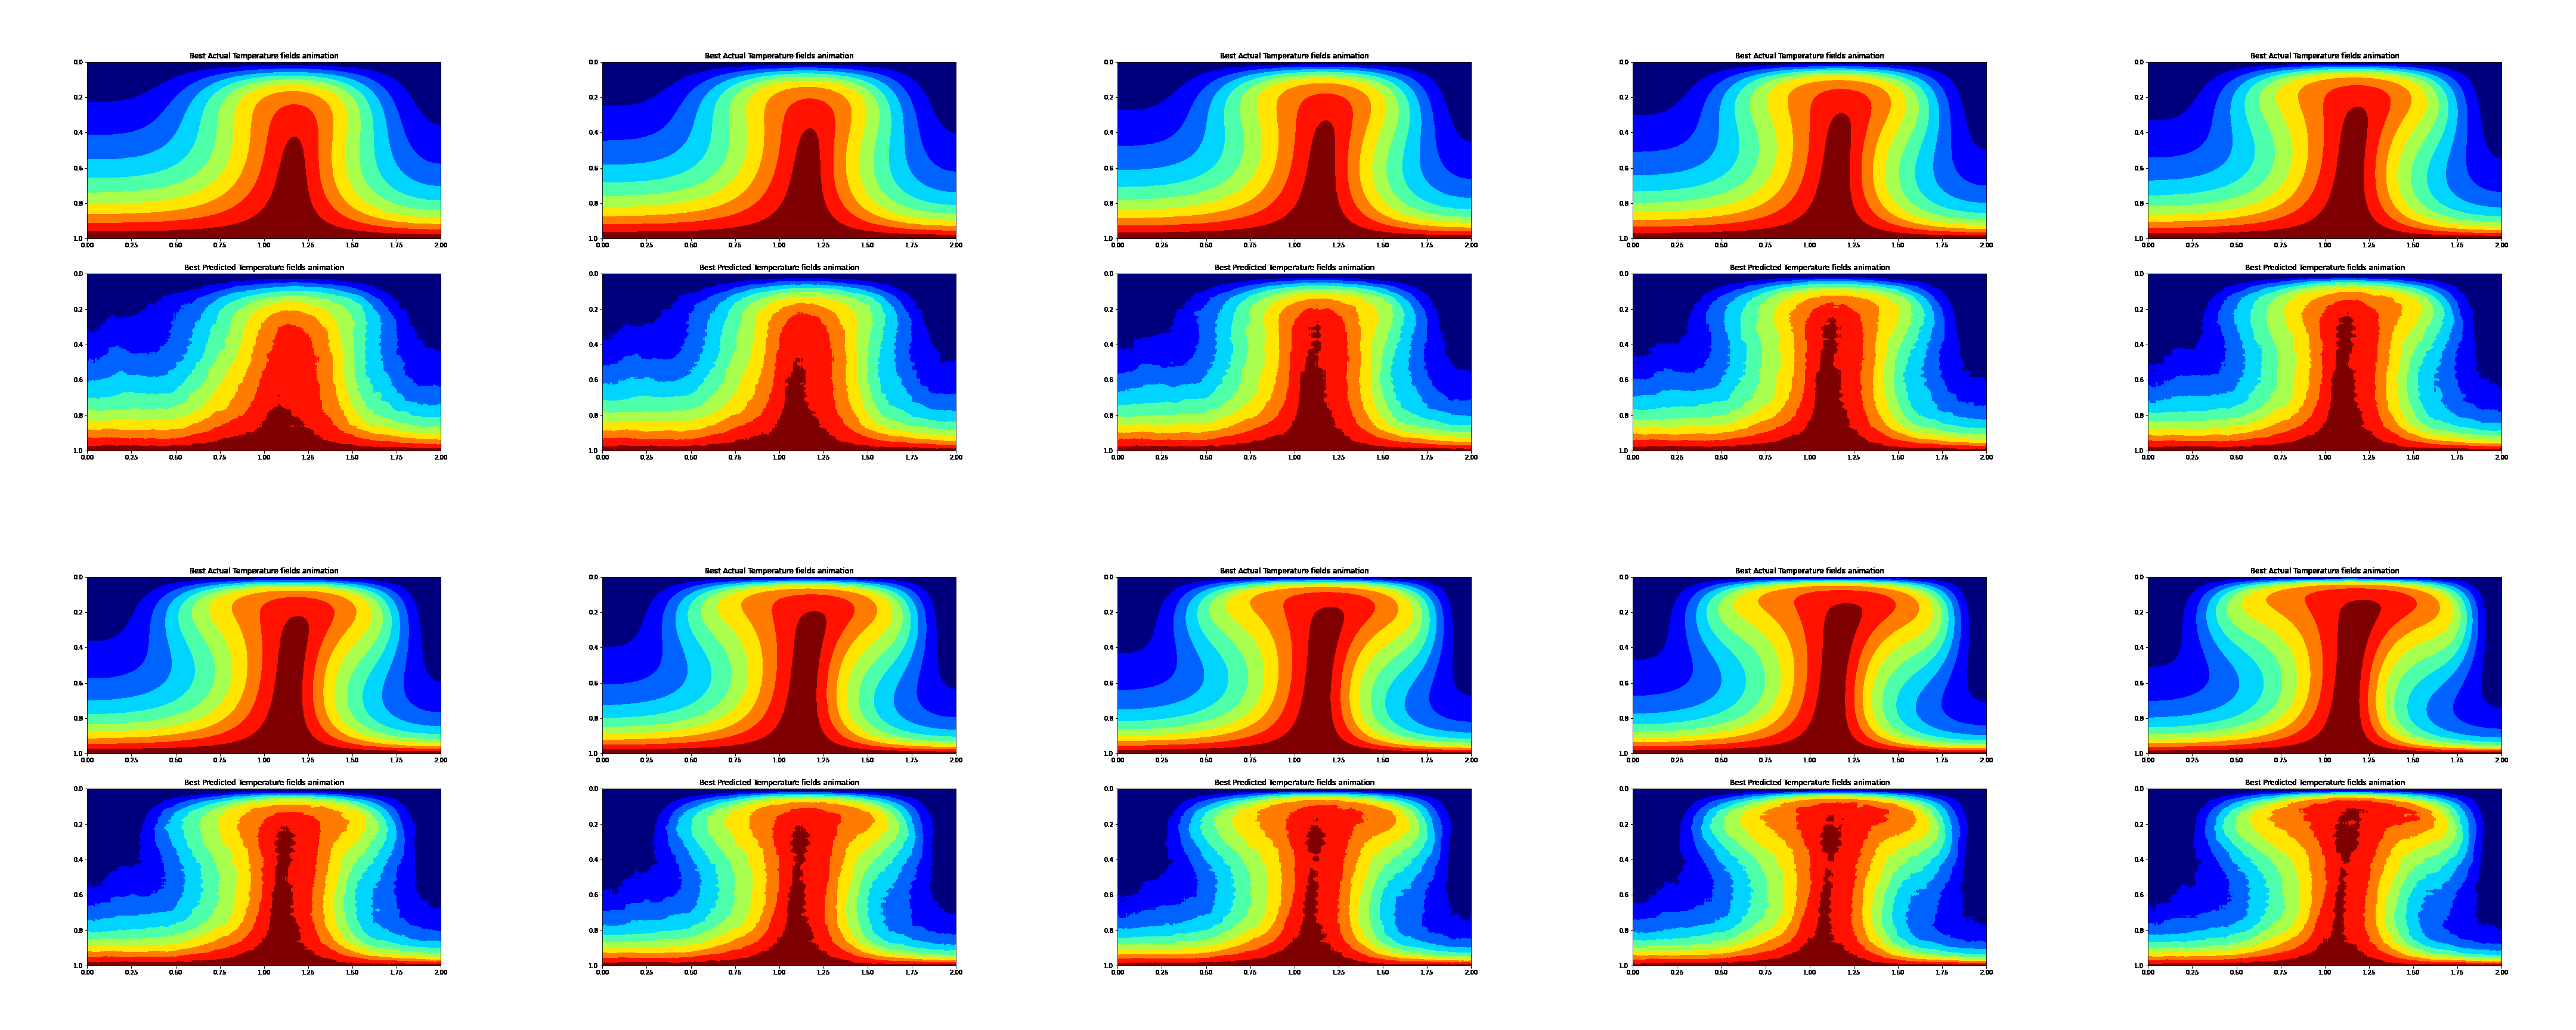
\includegraphics[scale=0.10]{figures/mantle_convection_images/limited_dataset/LSTM_Best_GIF_sheet.png}
\end{figure}



\begin{figure}[H]
    \centering
    \caption{Worst case animation sheet of LSTM trained with Limited Dataset (Link to this GIF: 
    \url{https://drive.google.com/file/d/1nINRk2Oh8rgQBLWio_b6R6I7T18e7Zi-/view?usp=sharing})}
    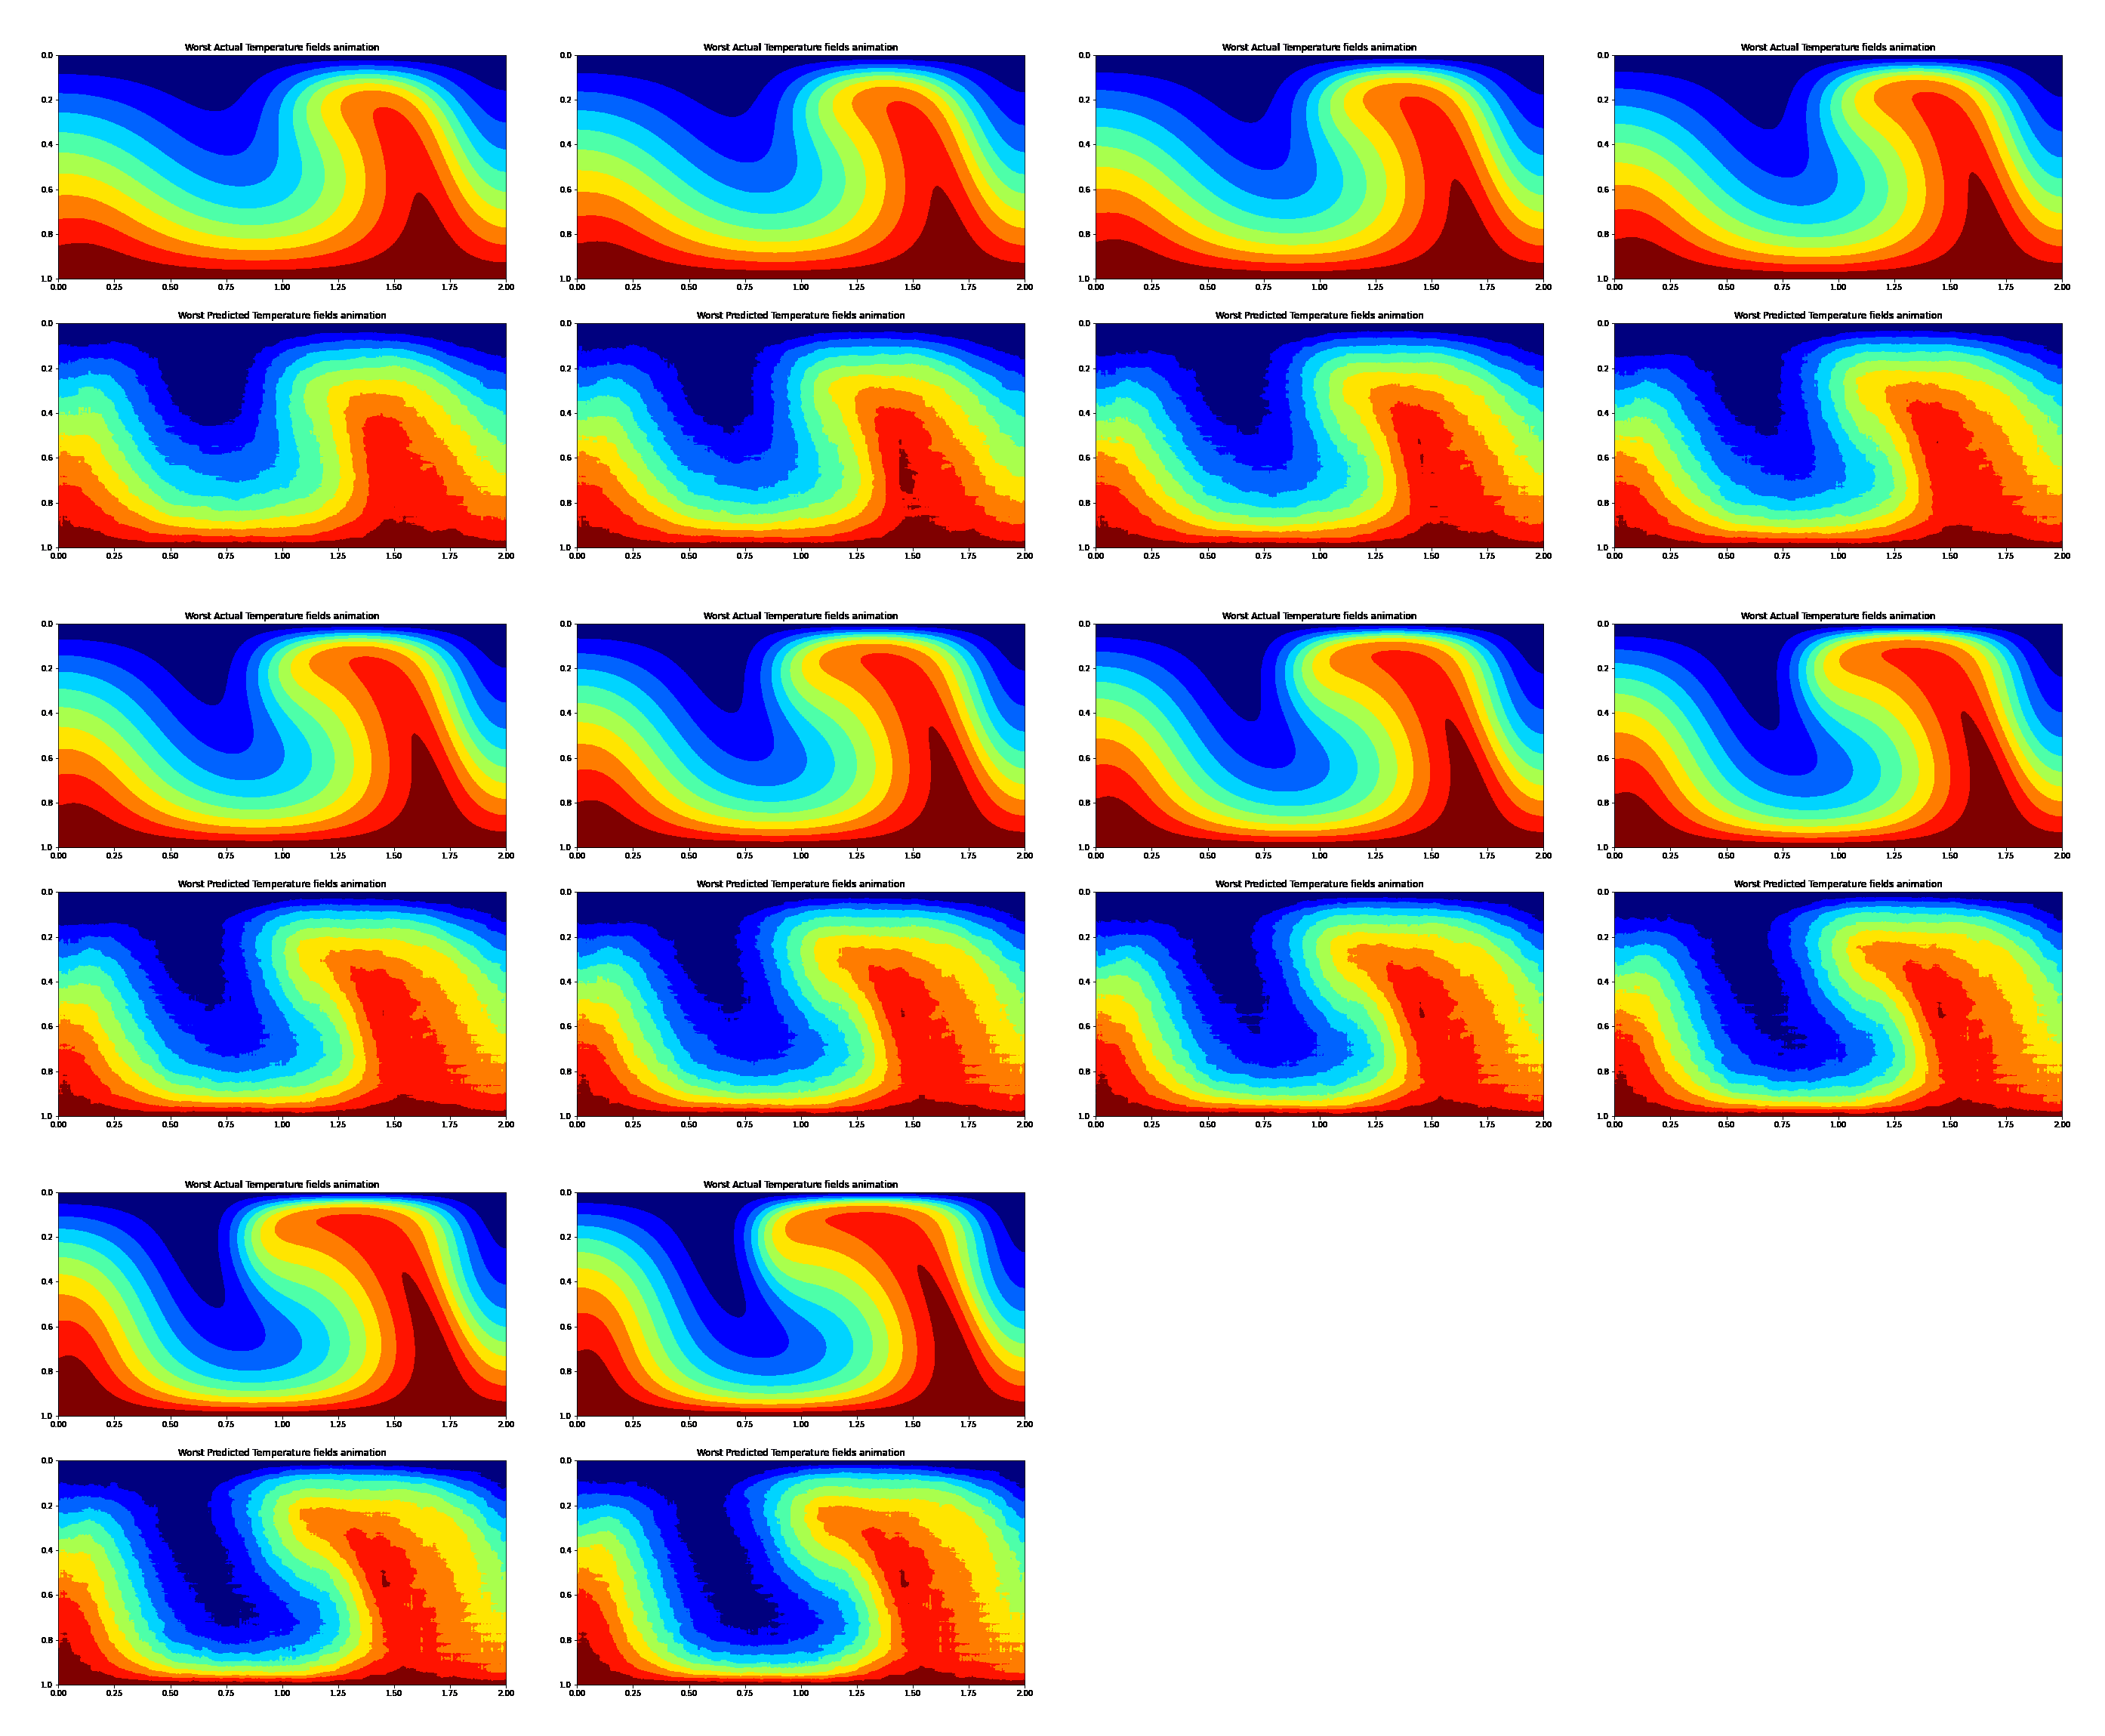
\includegraphics[scale=0.10]{figures/mantle_convection_images/limited_dataset/LSTM_Worst_GIF_sheet.png}
\end{figure}

To further evaluate the performance, we also applied POD to a sequence of predictions generated by LSTM in both the best case and the worst case, with the original time series and the compressed-decompressed version generated by ConvAE serving as contrast.

The following figures show the POD result in best case and the worst case:

\begin{figure}[H]
    \caption{Best case POD of LSTM trained with Limited Dataset.}
    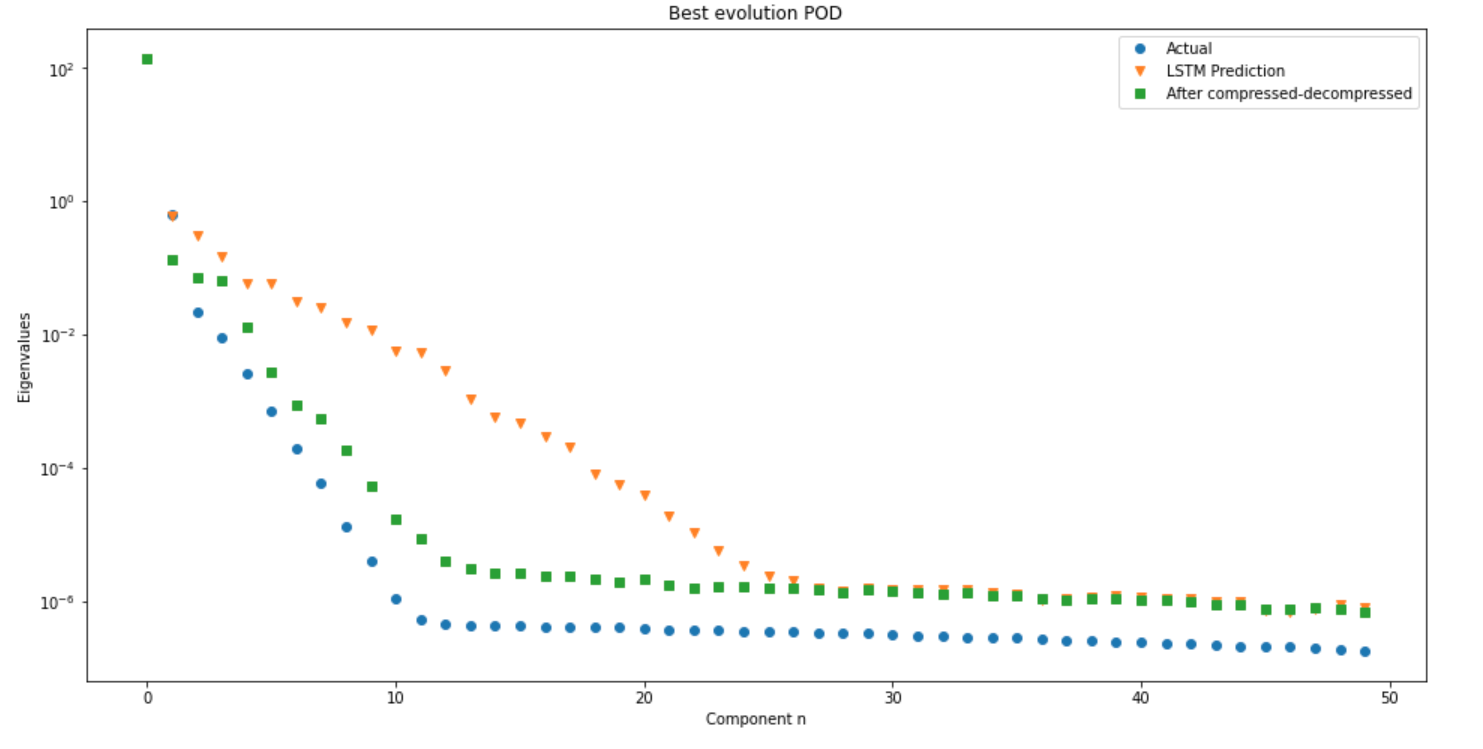
\includegraphics[scale=0.5]{figures/mantle_convection_images/limited_dataset/LSTM_Best_POD.png}
\end{figure}

\begin{figure}[H]
    \caption{Worst case POD of LSTM trained with Limited Dataset.}
    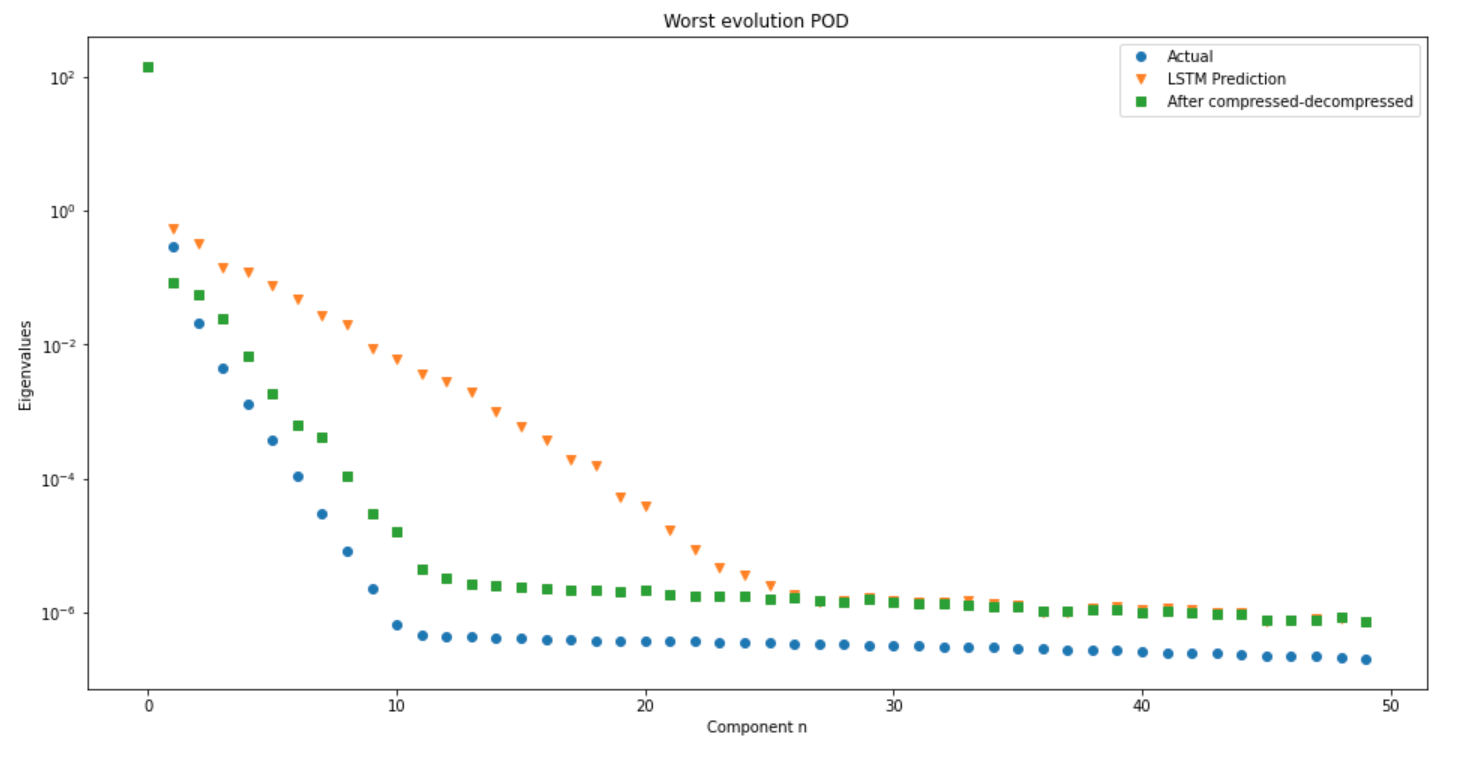
\includegraphics[scale=0.5]{figures/mantle_convection_images/limited_dataset/LSTM_Worst_POD.png}
\end{figure}

From the animations and the POD results, we can conclude that LSTM is able to capture the characteristics of the simulations even in its worst case. However, the simulations predicted using LSTM are less accurate and have more data loss compared with those predicted using FNN. There could be potential underfitting problem due to the lack of training data since only 80 samples are used for training.


\section{Mantle Convection Simulation on Larger Dataset}

To confirm if the low accuracy of LSTM is caused by the scarceness of data, a larger dataset is tested, whose only two differences with the limited dataset are that it now contains 903 simulations and it uses absolute time steps instead of adaptive time steps. However, even though it now uses absolute time steps, the distance between each of the consecutive time steps still varies.

For this section, the distance between time steps are not considered since we want to mainly focus on testing if the scarceness of data is the reason for the low accuracy of LSTM. Nevertheless, time steps will be used in the next section to create an interpolated dataset.

The larger dataset are randomly divided in the same way as the limited dataset for each of the three ML architectures in the following subsections.

\subsection{Compression of temperature fields}

The ConvAE used for compressing the temperature fields in this section has the same structure and the same set of hyperparamters as the one trained with limited dataset, except that the total number of epochs are now reduced from 1000 to 200 due to the constrains of the computation resources on Gadi.

In the following figures, some detailed test results from this ConvAE trained with larger dataset are presented:

\begin{figure}[H]
    \caption{Training loss and Validation loss of ConvAE trained with Larger Dataset.}
    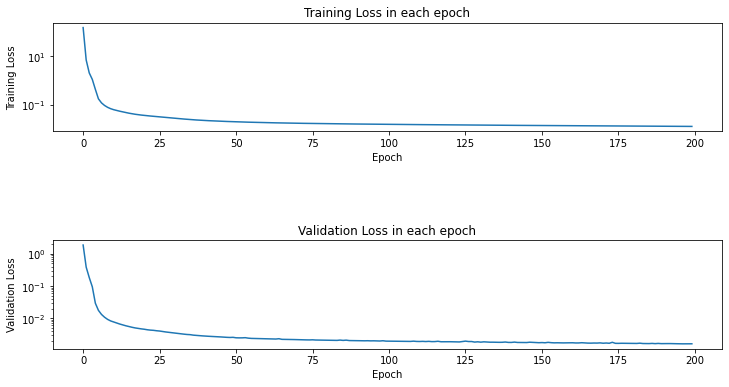
\includegraphics[scale=0.6]{figures/mantle_convection_images/larger_dataset/ConvAE_trainingData.png}
\end{figure}

\begin{figure}[H]
    \caption{Overall testing result of ConvAE trained with Larger Dataset.}
    
\includegraphics[scale=0.8]{figures/mantle_convection_images/larger_dataset/ConvAE_OverallTesting.png}
\end{figure}

\begin{figure}[H]
\centering
\begin{subfigure}{0.45\textwidth}
    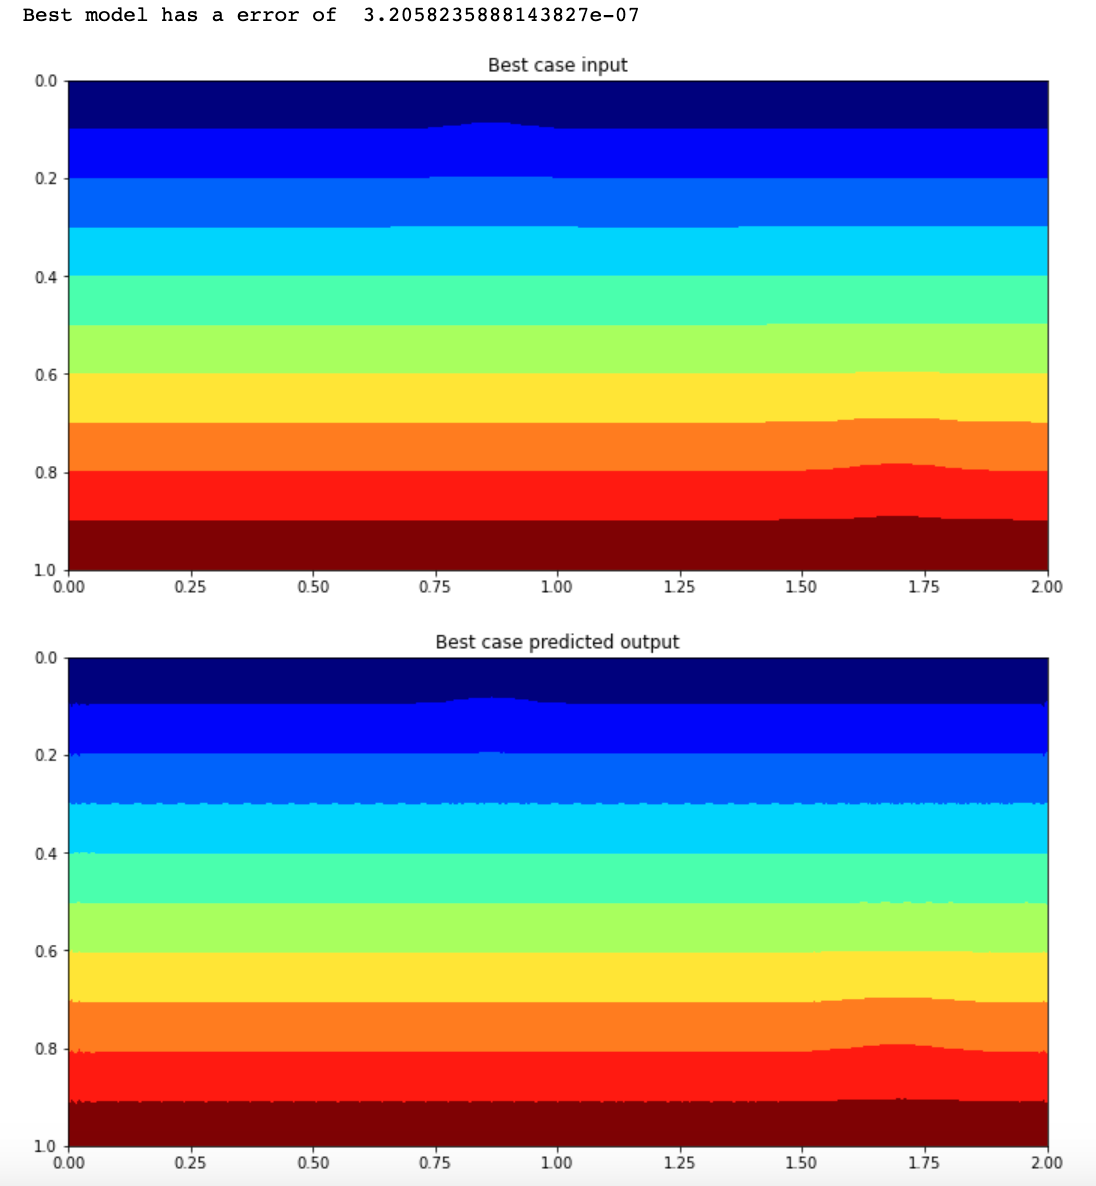
\includegraphics[width=\textwidth]{figures/mantle_convection_images/larger_dataset/ConvAE_Best.png}
    \caption{Best Case of ConvAE trained with Larger Dataset.}
\end{subfigure}
\hfill
\begin{subfigure}{0.45\textwidth}
    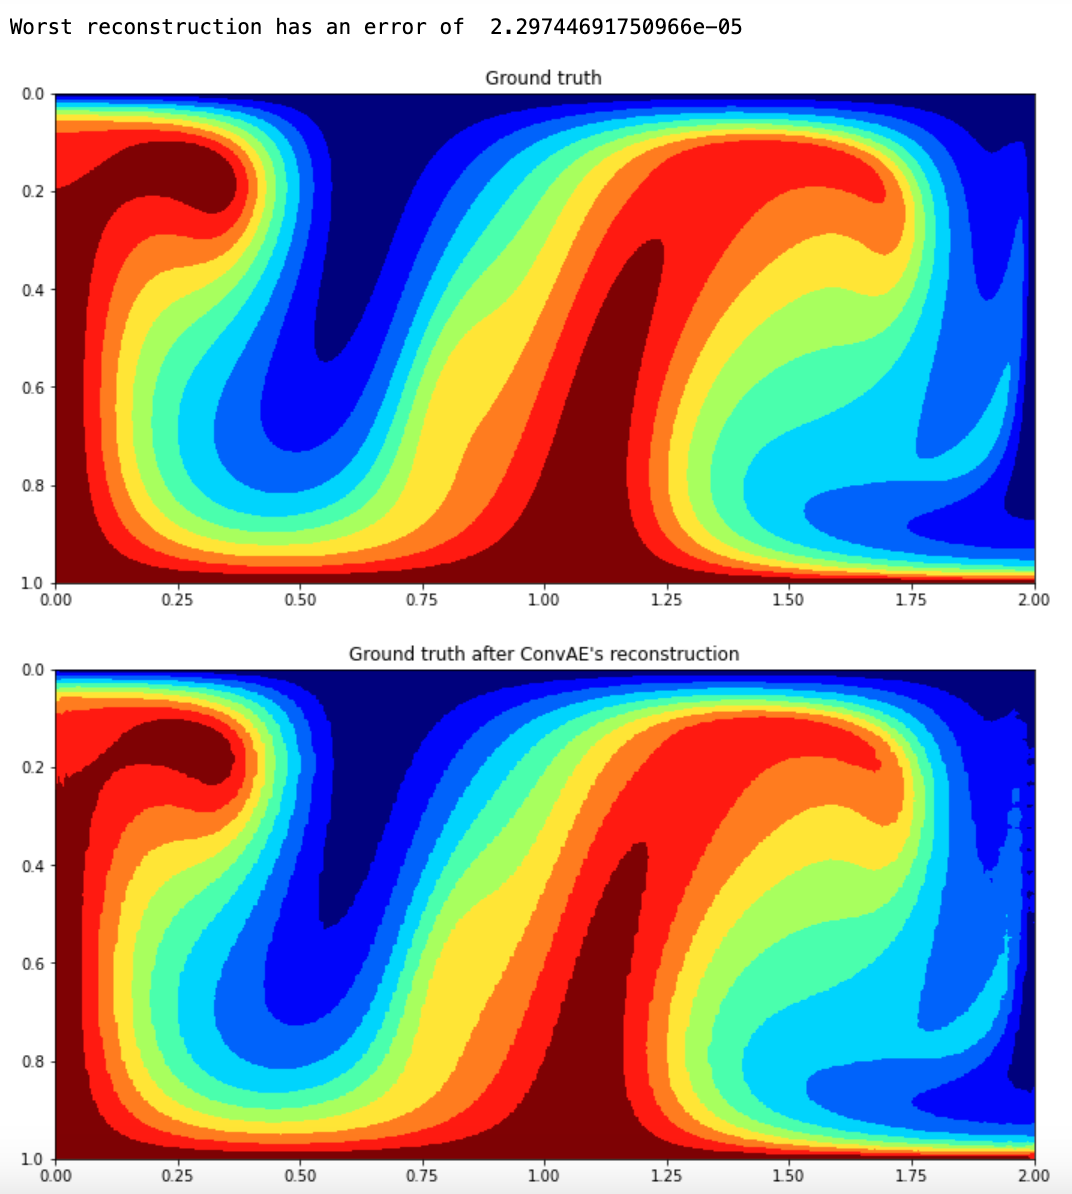
\includegraphics[width=\textwidth]{figures/mantle_convection_images/larger_dataset/ConvAE_Worst.png}
    \caption{Worst Case of ConvAE trained with Larger Dataset.}
\end{subfigure}
        
\caption{Best case and worst case using ConvAE.}
\end{figure}

Overall, the performance of this ConvAE is similar to the one trained with limited dataset: reconstruction loss are low and no overfitting occurs.


\subsection{Fully Connected Neural Network for Prediction}

The FNN in this section also has the same structure and the same set of hyperparamters as the one trained with limited dataset, except that the total number of epochs are reduced from 1000 to 200 as well.

The results are presented in the following figures:

\begin{figure}[H]
    \caption{Training loss and Validation loss of FNN trained with Larger Dataset.}
    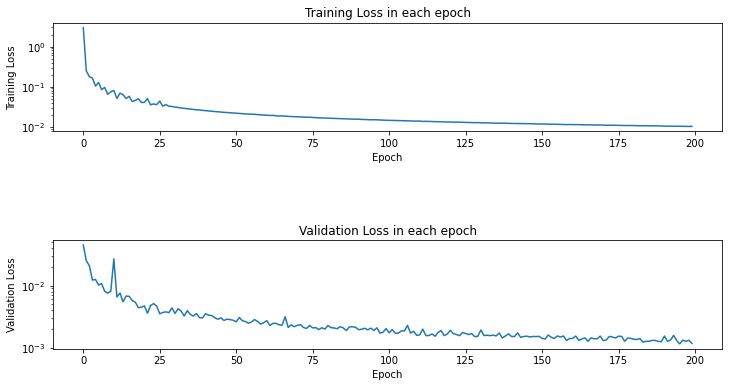
\includegraphics[scale=0.6]{figures/mantle_convection_images/larger_dataset/FNN_trainingData.png}
\end{figure}

\begin{figure}[H]
    \caption{Overall testing result of FNN trained with Larger Dataset.}
    
\includegraphics[scale=0.8]{figures/mantle_convection_images/larger_dataset/FNN_OverallTesting.png}
\end{figure}

\begin{figure}[H]
    \caption{Best case original output, original output after ConvAE's compression-decompression, and predicted output of FNN trained with Larger Dataset.}
    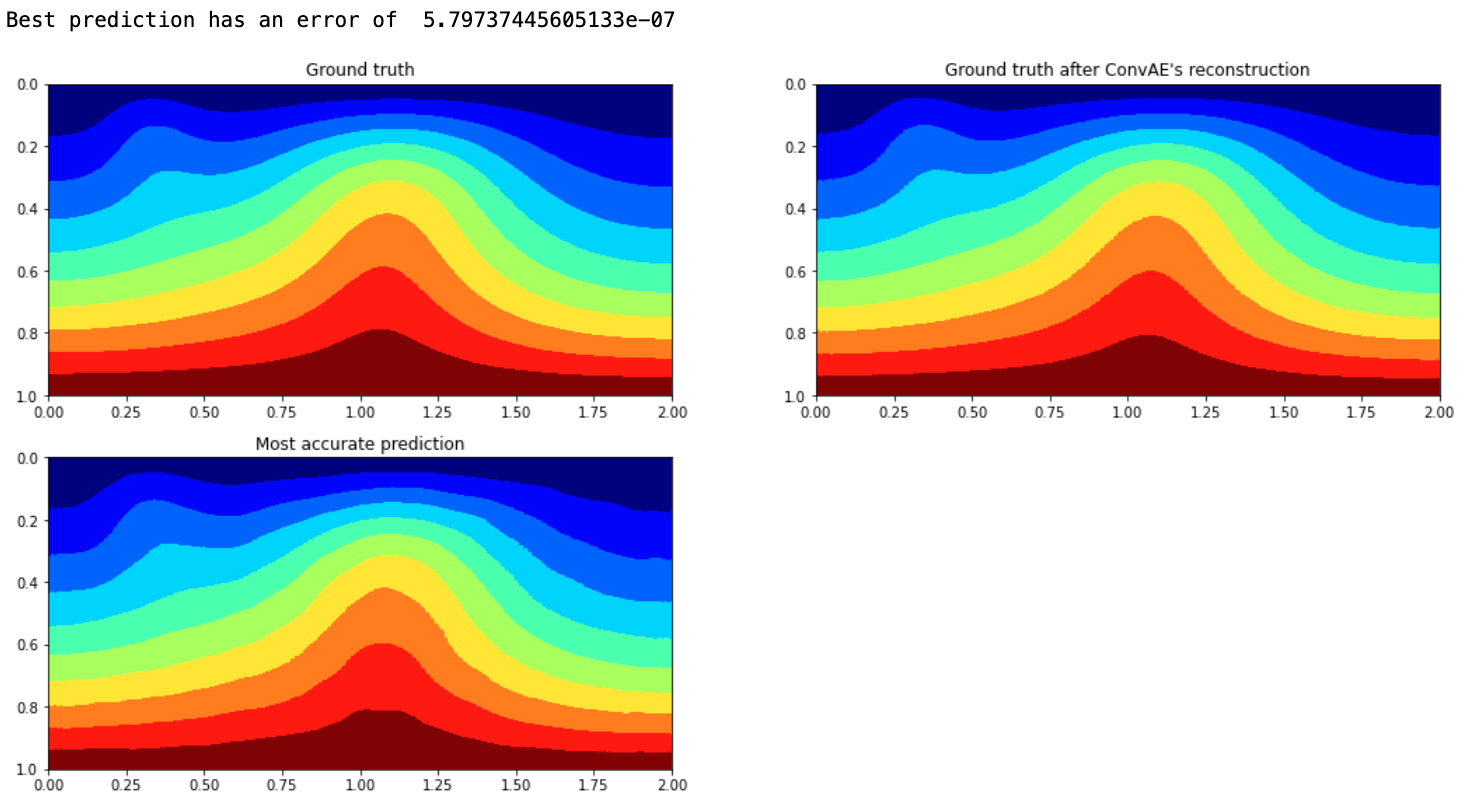
\includegraphics[scale=0.5]{figures/mantle_convection_images/larger_dataset/FNN_Best.png}
\end{figure}

\begin{figure}[H]
    \caption{Worst case original output, original output after ConvAE's compression-decompression, and predicted output of FNN trained with Larger Dataset.}
    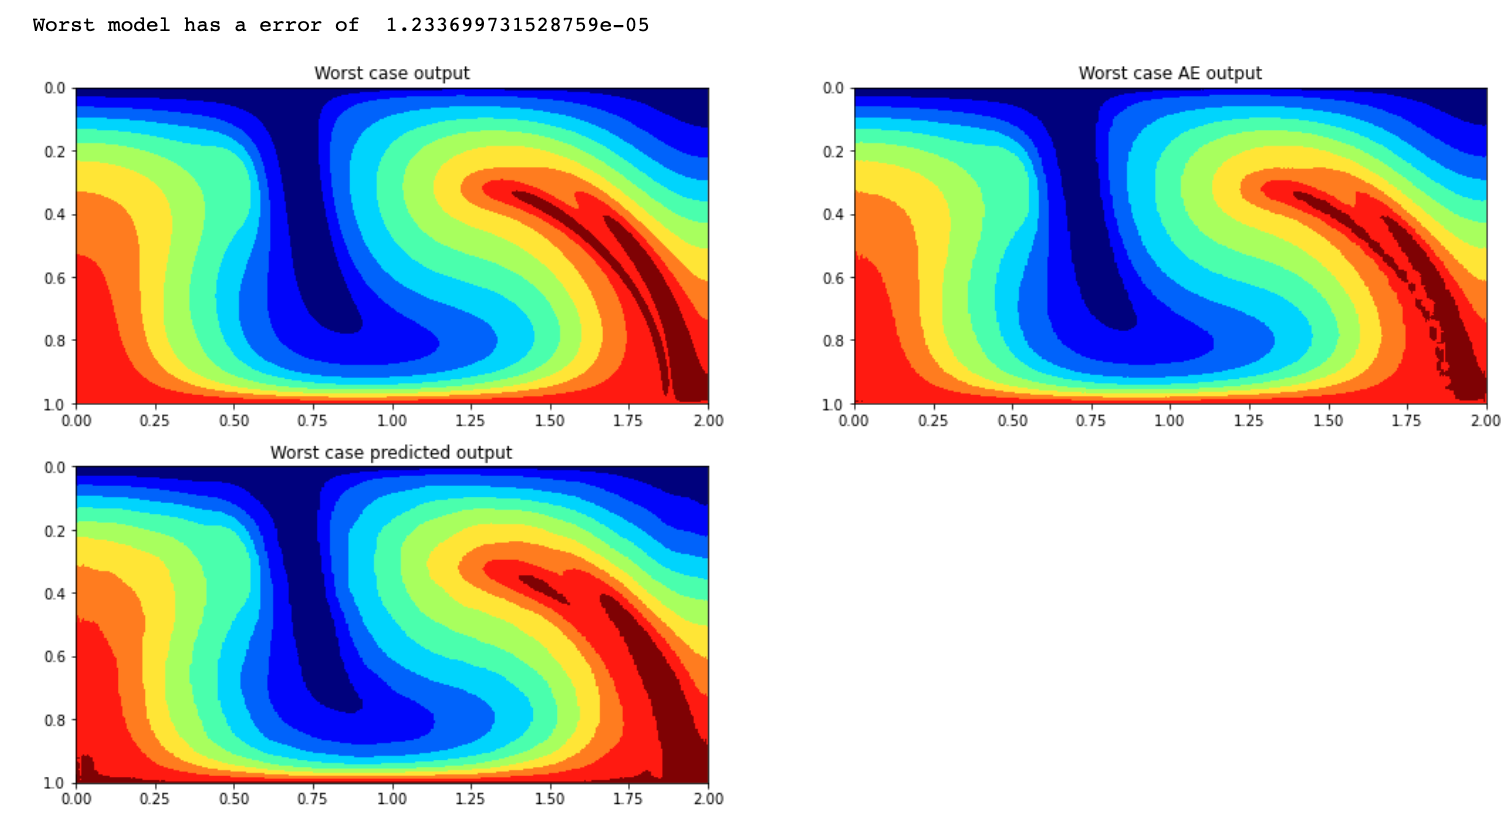
\includegraphics[scale=0.5]{figures/mantle_convection_images/larger_dataset/FNN_Worst.png}
\end{figure}

The above result of this FNN are similar to the one trained with limited dataset: the loss values are low and no overfitting occurs. There are still some small information loss, which is now confirmed as caused by the loss of data generated during the compression-decompression process of ConvAE.

Again, two animations representing the best case and the worst case when predicting the entire simulation using "One-for-All" (use $T1$ from dataset $\rightarrow$ get predicted $T2$ $\rightarrow$ use predicted $T2$ $\rightarrow$ get predicted $T3$ $\rightarrow$ ...) are generated.

The following figures show 10\% of the sprite sheets converted from the original GIF animations (Every 10th frame), along with the POD result for the best case and worst case:

\begin{figure}[H]
    \centering
    \caption{Best case animation sheet of FNN trained with Larger Dataset (Link to this GIF: \url{https://drive.google.com/file/d/1LxuwXxEoG5xsYzLYn6n6-mUfoP8A3IC2/view?usp=sharing})}
    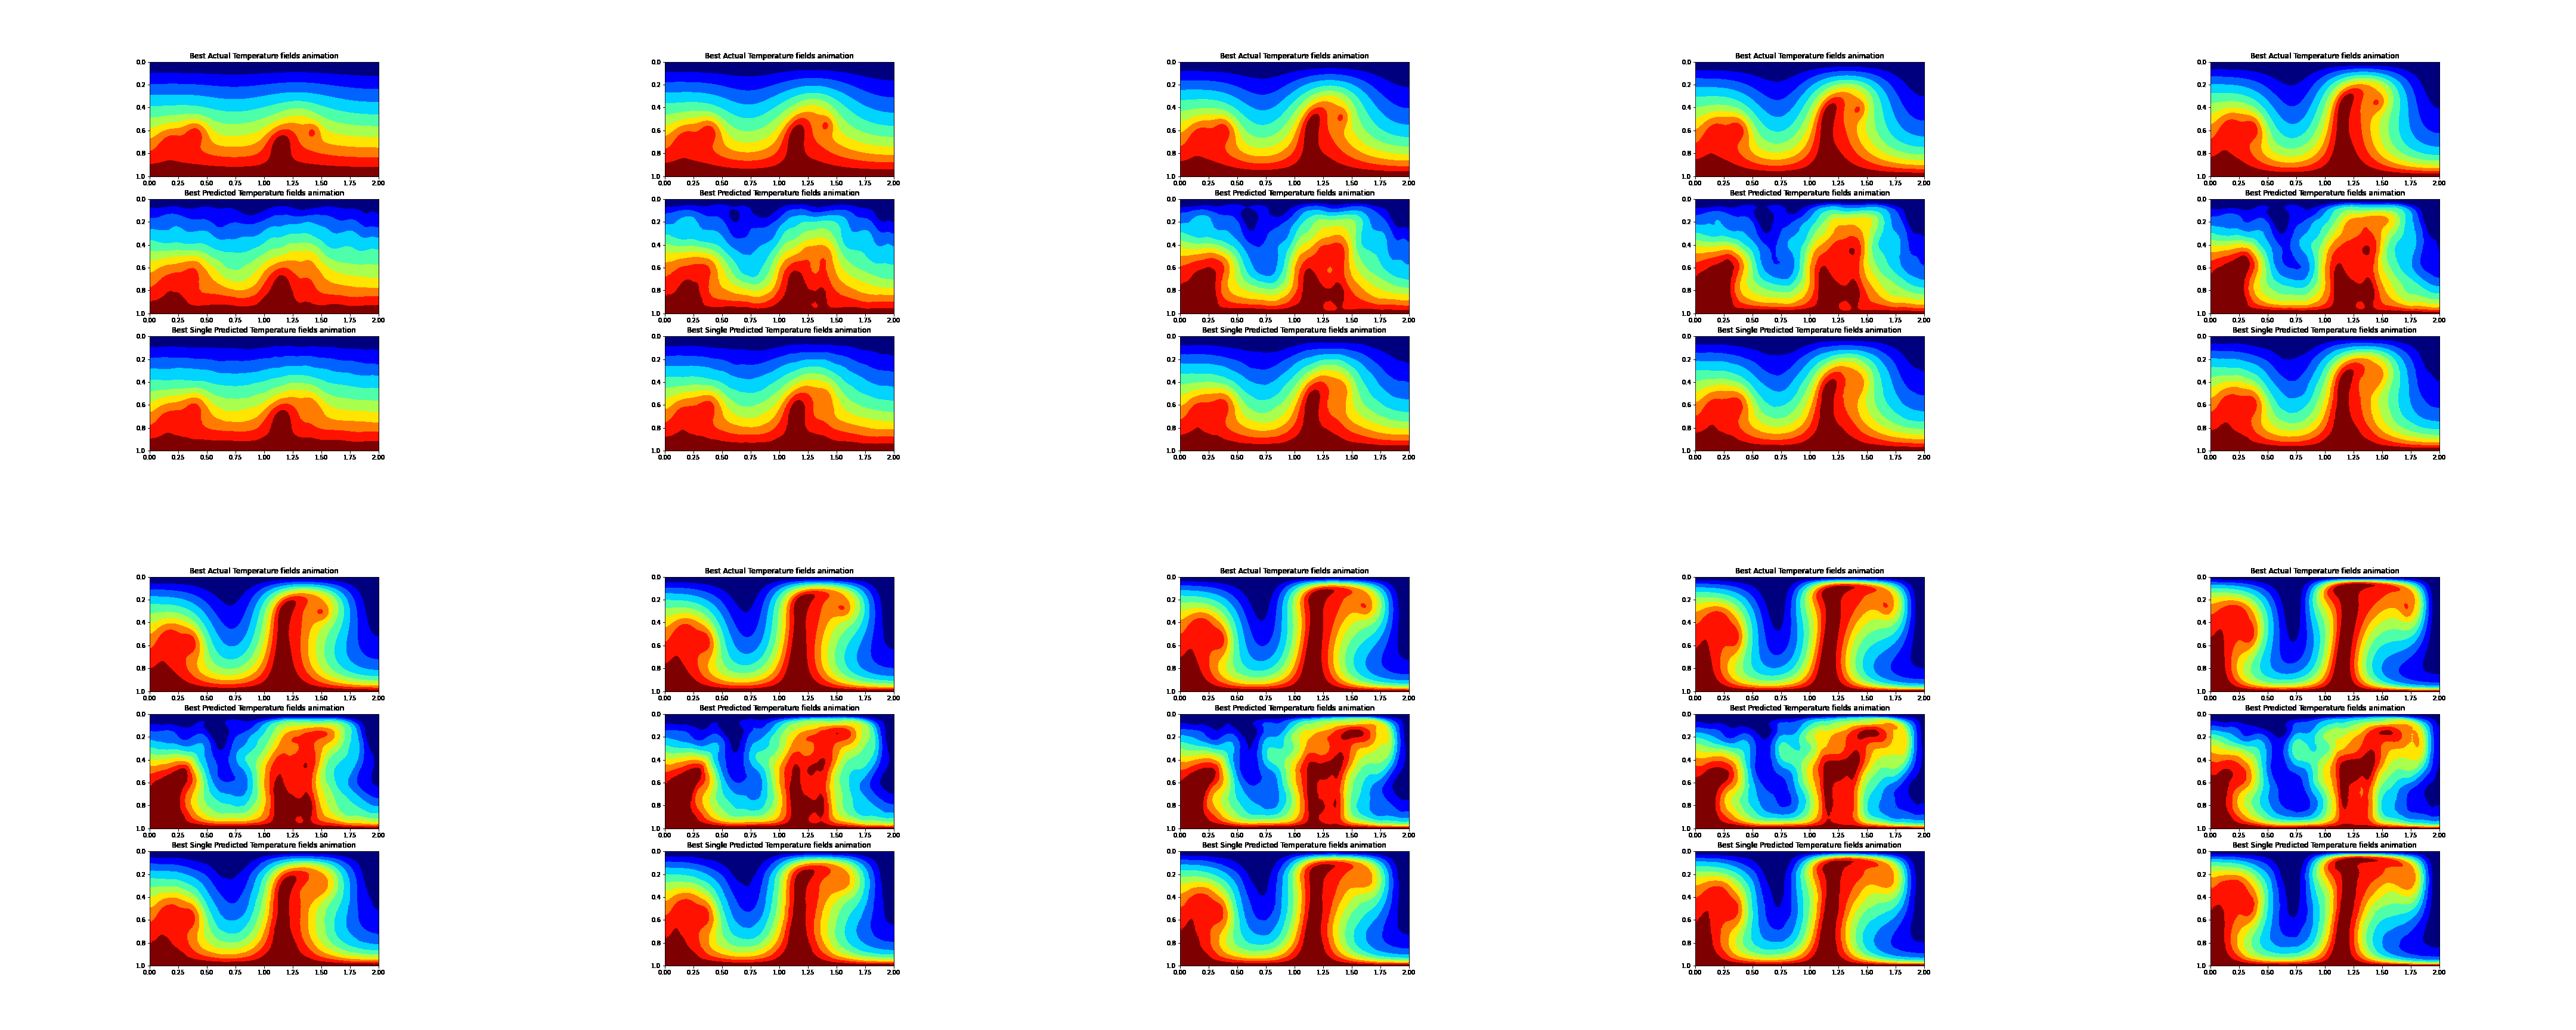
\includegraphics[scale=0.10]{figures/mantle_convection_images/larger_dataset/FNN_Best_GIF_sheet.png}
\end{figure}

\begin{figure}[H]
    \centering
    \caption{Worst case animation sheet of FNN trained with Larger Dataset (Link to this GIF: 
    \url{https://drive.google.com/file/d/1vwfL_n6ANnkJEY3B8a024SF_yQ35Hkxu/view?usp=sharing})}
    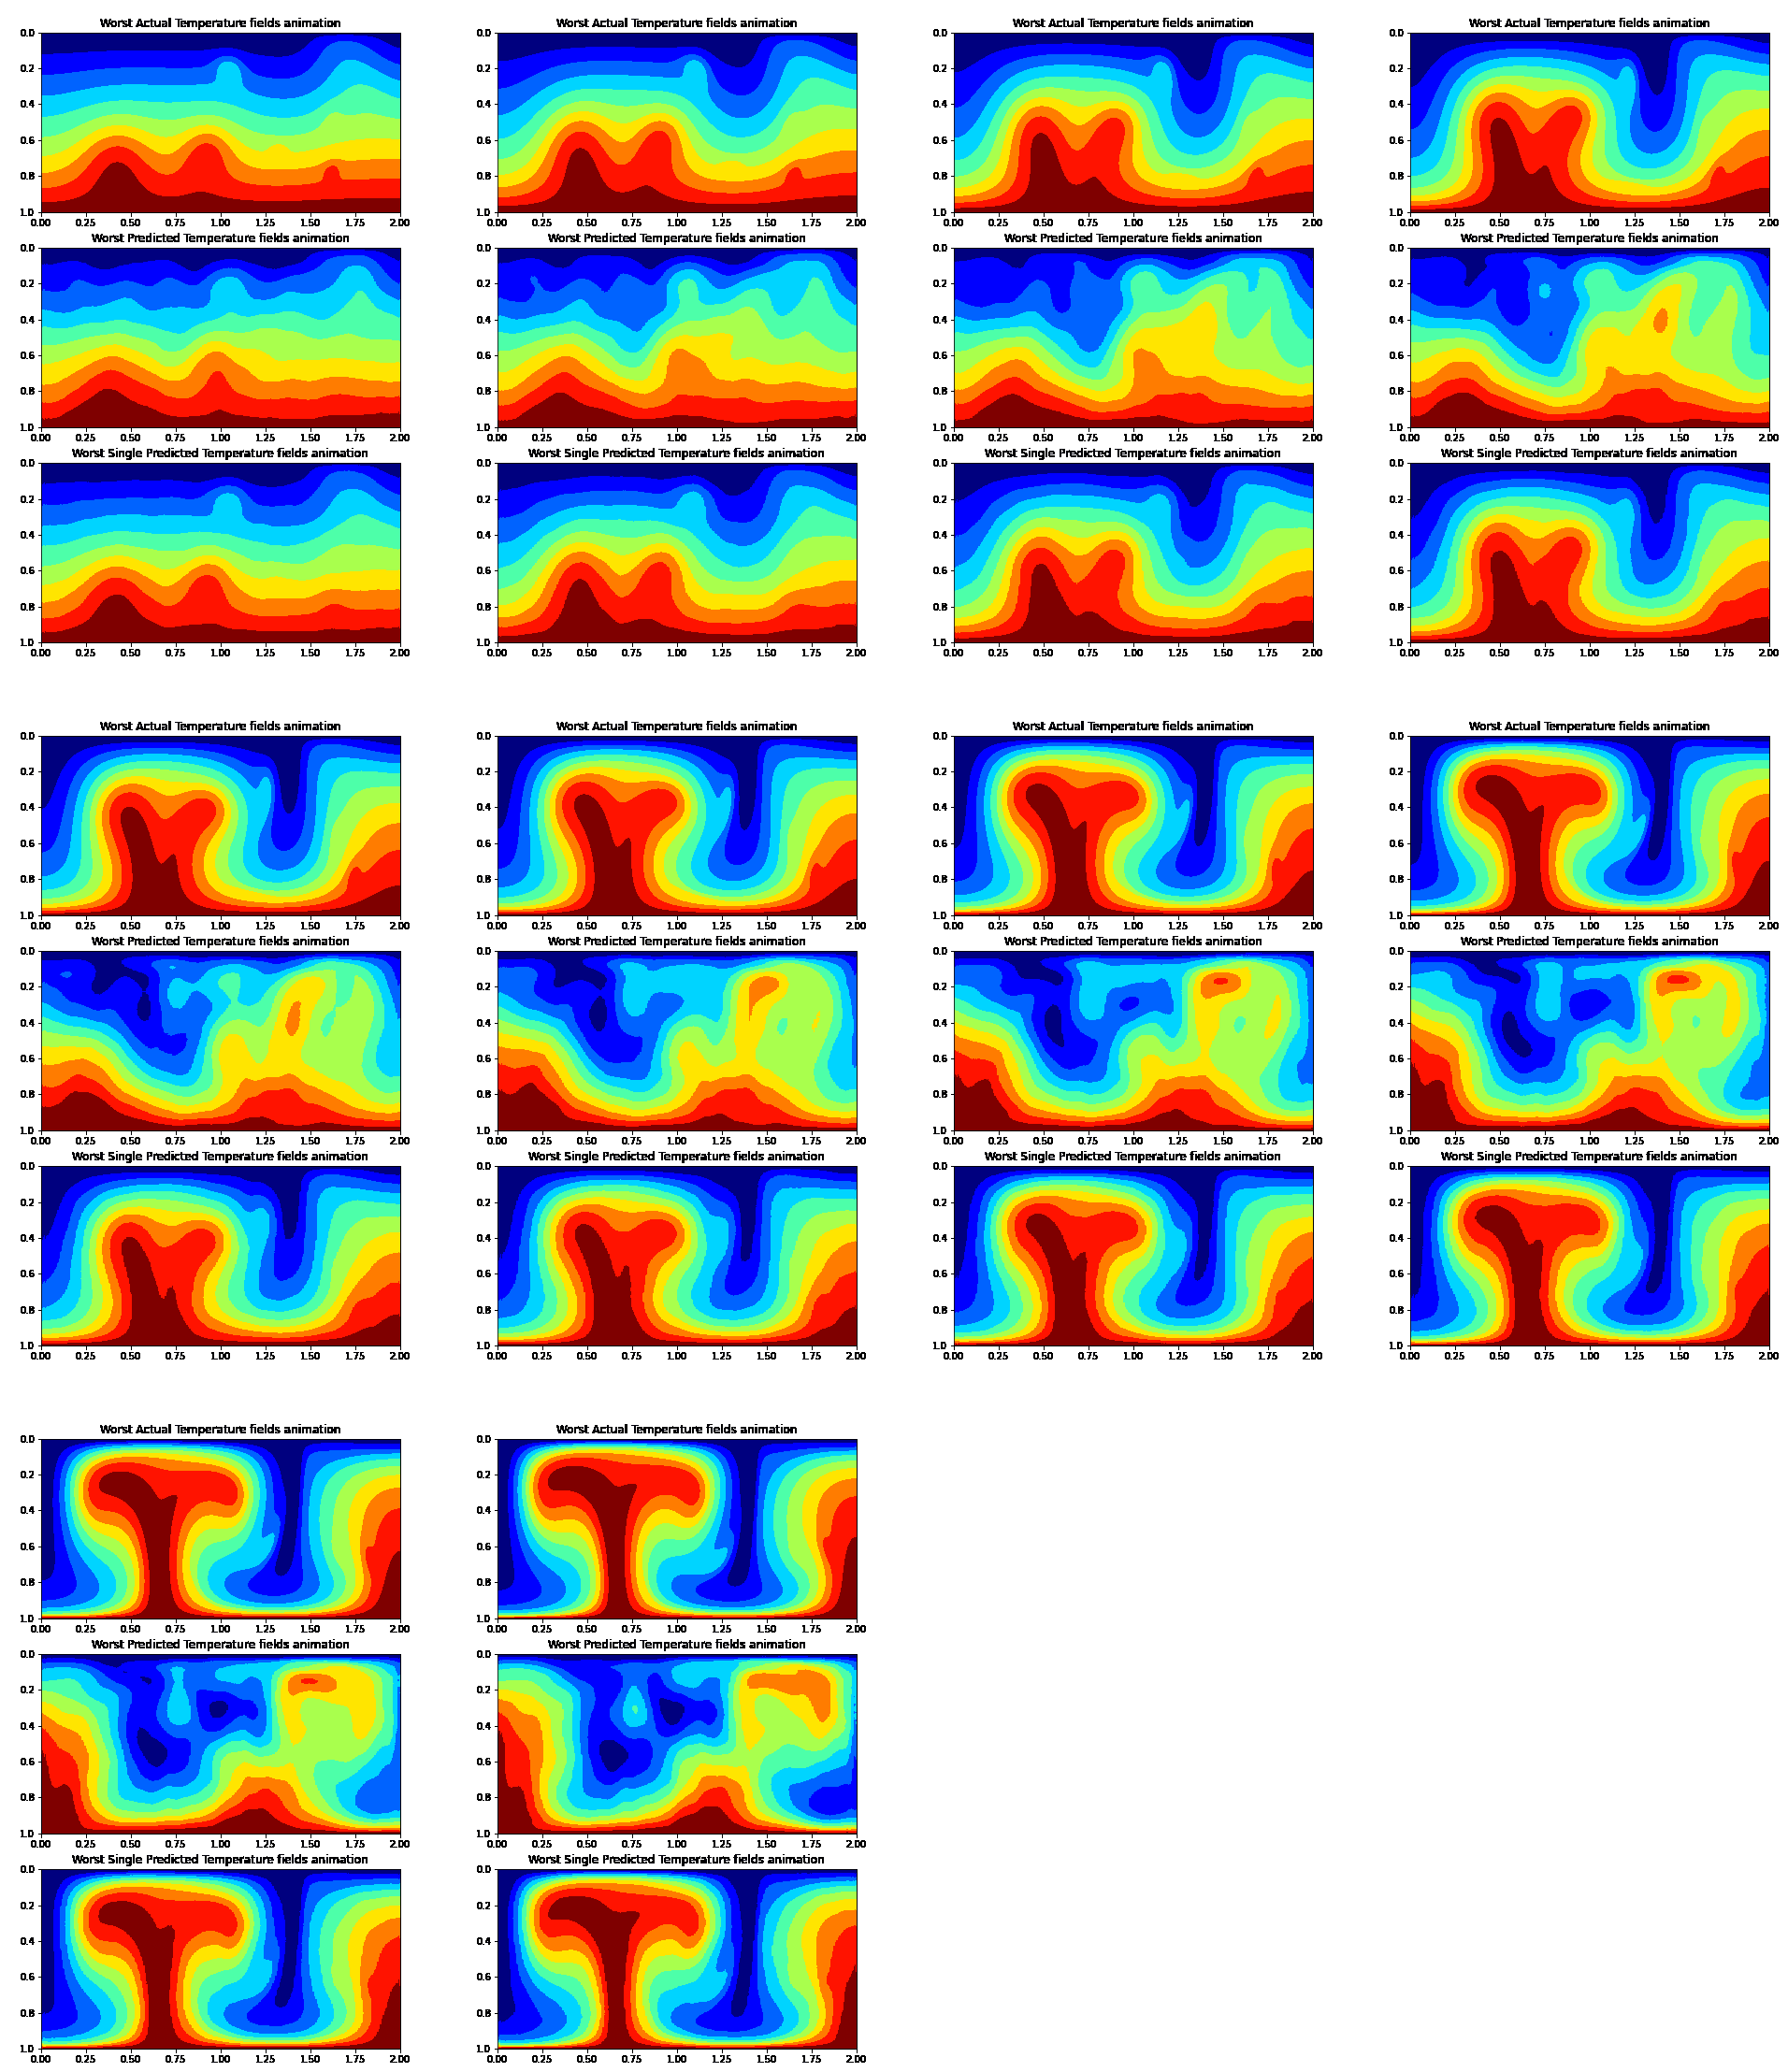
\includegraphics[scale=0.10]{figures/mantle_convection_images/larger_dataset/FNN_Worst_GIF_sheet.png}
\end{figure}


\begin{figure}[H]
    \caption{Best case POD of FNN trained with Larger Dataset.}
    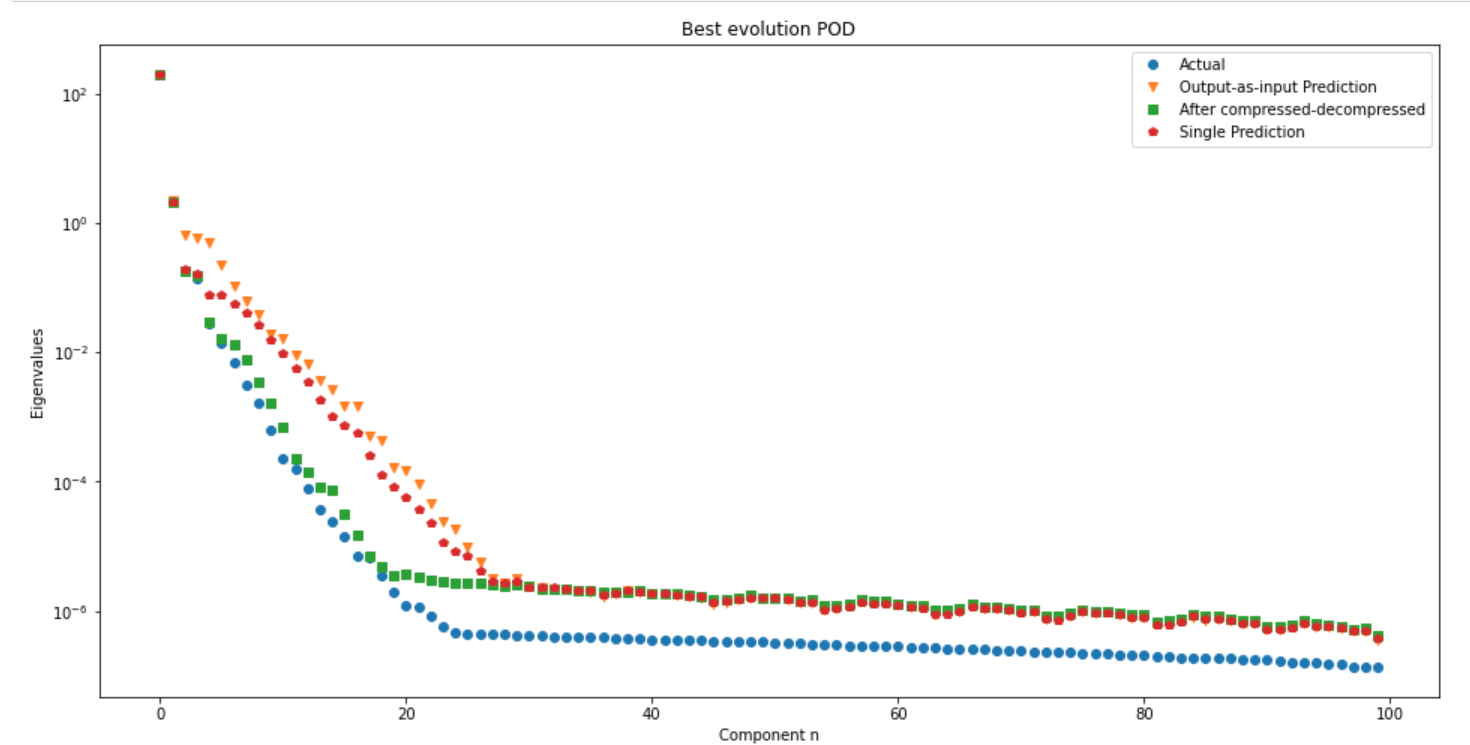
\includegraphics[scale=0.5]{figures/mantle_convection_images/larger_dataset/FNN_Best_POD.png}
\end{figure}

\begin{figure}[H]
    \caption{Worst case POD of FNN trained with Larger Dataset.}
    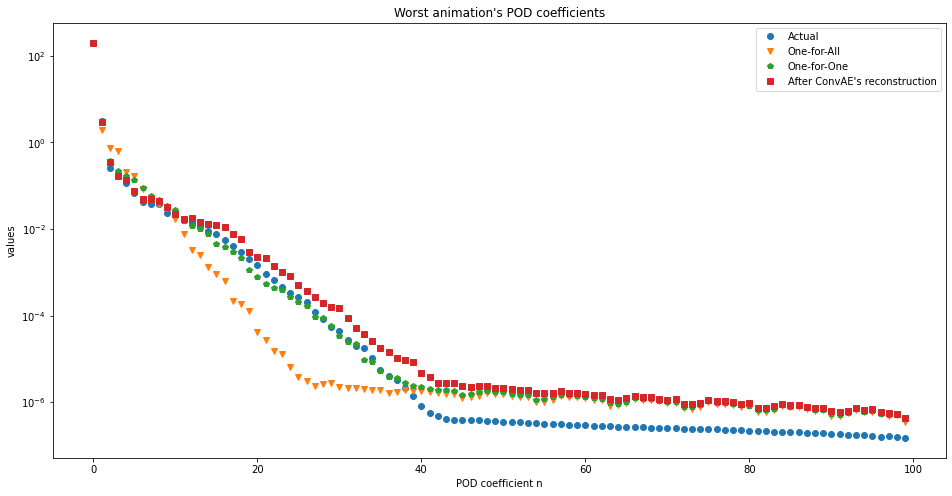
\includegraphics[scale=0.5]{figures/mantle_convection_images/larger_dataset/FNN_Worst_POD.png}
\end{figure}

We can observe that the increasing size of the training data does not improve the quality of the animations when predicting the entire simulations using the first method. Also, apart from the information loss, the problem of the predicted GIFs moving too fast or too slow still exists.


\subsection{Long Short-Term Memory (LSTM) for Prediction}

The LSTM in this section also has the same structure and the same set of hyperparamters as the one trained with limited dataset, except that the total number of epochs are reduced from 200 to 100.

The results are presented in the following figures:

\begin{figure}[H]
    \caption{Training loss and Validation loss of LSTM trained with Larger Dataset.}
    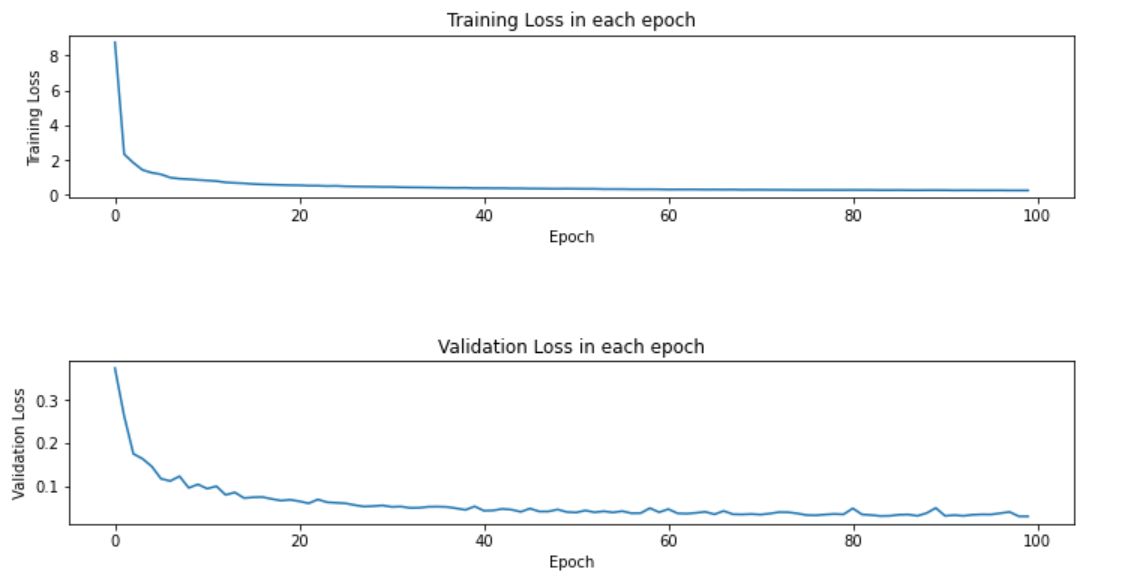
\includegraphics[scale=0.6]{figures/mantle_convection_images/larger_dataset/LSTM_trainingData.png}
\end{figure}

\begin{figure}[H]
    \caption{Overall testing result of LSTM trained with Larger Dataset.}
    \includegraphics[scale=0.8]{figures/mantle_convection_images/larger_dataset/LSTM_OverallTesting.png}
\end{figure}

\begin{figure}[H]
    \caption{Best case original output, original output after ConvAE's compression-decompression, and predicted output of LSTM trained with Larger Dataset.}
    \includegraphics[scale=0.5]{figures/mantle_convection_images/larger_dataset/LSTM_Best.png}
\end{figure}

\begin{figure}[H]
    \caption{Worst case original output, original output after ConvAE's compression-decompression, and predicted output of LSTM trained with Larger Dataset.}
    \includegraphics[scale=0.5]{figures/mantle_convection_images/larger_dataset/LSTM_Worst.png}
\end{figure}


From the above figures, we can see that the loss of the best case and the worst case for this LSTM are in the same level as the one trained with limited dataset given 10 times of the training data, which means that the low accuracy of LSTM is not caused by some potential underfitting problem as discussed in the last section.

For better visualisation as well, two animations representing the best case and the worst case when predicting the rest of the simulation using the first 50 temperature fields are generated.

The following figures show 20\% of the sprite sheets converted from the original GIF animations (Every 5th frame), along with the POD result for the best case and worst case:

\begin{figure}[H]
    \centering
    \caption{Best case animation sheet of LSTM trained with Larger Dataset (Link to this GIF: \url{https://drive.google.com/file/d/1UFYSPVLT1wRsKM5GAdCz0JQLZF8OKNUc/view?usp=sharing})}
    \includegraphics[scale=0.10]{figures/mantle_convection_images/larger_dataset/LSTM_Best_GIF_sheet.png}
\end{figure}



\begin{figure}[H]
    \centering
    \caption{Worst case animation sheet of LSTM trained with Larger Dataset (Link to this GIF: 
    \url{https://drive.google.com/file/d/1SbzjPwwe7FCu7JCJru8UYHOu9j6uVfZd/view?usp=sharing})}
    \includegraphics[scale=0.10]{figures/mantle_convection_images/larger_dataset/LSTM_Worst_GIF_sheet.png}
\end{figure}


\begin{figure}[H]
    \caption{Best case POD of LSTM trained with Larger Dataset.}
    \includegraphics[scale=0.5]{figures/mantle_convection_images/larger_dataset/LSTM_Best_POD.png}
\end{figure}

\begin{figure}[H]
    \caption{Worst case POD of LSTM trained with Larger Dataset.}
    \includegraphics[scale=0.5]{figures/mantle_convection_images/larger_dataset/LSTM_Worst_POD.png}
\end{figure}

From the animations and the POD results, we can now confirmed that LSTM is able to capture most of characteristics of the simulations even in its worst case and the simulations predicted using LSTM are less accurate compared with those predicted using FNN.


\section{Mantle Convection Simulation on Interpolated Dataset}

To confirm if the problem of the predicted GIFs moving too fast or too slow is caused by the varying distance between time steps, an interpolated dataset is created using the larger dataset in the last section.

The interpolation process is done for each of the simulation separately by generating a sequence of temperature fields with equal distance between their consecutive time steps. The resulting sequence of time steps for every interpolated simulations are the same by giving a start time step (close to the minimum time step), an end time step (close to the maximum time step) and the number of samples (=100) to generate a new evenly spaced time step sequence to interpolate with. In order to retrieve the temperature field at the target time step, the temperature fields at two nearest time steps are searched for and the target temperature field is generated by interpolating between these two temperature fields.

After the interpolation process, we are able to get an interpolation dataset where every simulation has the same time steps.

The interpolated dataset are also randomly divided in the same way as the limited dataset for each of the three ML architectures in the following subsections.


\subsection{Compression of temperature fields}

The ConvAE used for compressing the temperature fields in this section has the same structure and the same set of hyperparameters as the one trained with the original larger dataset.

In the following figures, some detailed test results from this ConvAE trained with interpolated dataset are presented:

\begin{figure}[H]
    \caption{Training loss and Validation loss of ConvAE trained with Interpolated Dataset.}
    \includegraphics[scale=0.6]{figures/mantle_convection_images/larger_dataset_interpolated/ConvAE_trainingData.png}
\end{figure}

\begin{figure}[H]
    \caption{Overall testing result of ConvAE trained with Interpolated Dataset.}
    \includegraphics[scale=0.8]{figures/mantle_convection_images/larger_dataset_interpolated/ConvAE_OverallTesting.png}
\end{figure}

\begin{figure}[H]
\centering
\begin{subfigure}{0.45\textwidth}
    \includegraphics[width=\textwidth]{figures/mantle_convection_images/larger_dataset_interpolated/ConvAE_Best.png}
    \caption{Best Case of ConvAE trained with Interpolated Dataset.}
\end{subfigure}
\hfill
\begin{subfigure}{0.45\textwidth}
    \includegraphics[width=\textwidth]{figures/mantle_convection_images/larger_dataset_interpolated/ConvAE_Worst.png}
    \caption{Worst Case of ConvAE trained with Interpolated Dataset.}
\end{subfigure}
        
\caption{Best case and worst case using ConvAE.}
\end{figure}

We can observe that the performance of this ConvAE is better than the one trained with the original larger dataset since it has a total loss that is 3 times lower than the one in the last section (0.0005 to 0.0016). This could imply that the interpolated data make the training process of ConvAE easier given the same size of data. 


\subsection{Fully Connected Neural Network for Prediction}

The FNN in this section also has the same structure and the same set of hyperparameters as the one trained with the original larger dataset.

The results are presented in the following figures:

\begin{figure}[H]
    \caption{Training loss and Validation loss of FNN trained with Interpolated Dataset.}
    \includegraphics[scale=0.6]{figures/mantle_convection_images/larger_dataset_interpolated/FNN_trainingData.png}
\end{figure}

\begin{figure}[H]
    \caption{Overall testing result of FNN trained with Interpolated Dataset.}
    \includegraphics[scale=0.8]{figures/mantle_convection_images/larger_dataset_interpolated/FNN_OverallTesting.png}
\end{figure}

\begin{figure}[H]
    \caption{Best case original output, original output after ConvAE's compression-decompression, and predicted output of FNN trained with Interpolated Dataset.}
    \includegraphics[scale=0.5]{figures/mantle_convection_images/larger_dataset_interpolated/FNN_Best.png}
\end{figure}

\begin{figure}[H]
    \caption{Worst case original output, original output after ConvAE's compression-decompression, and predicted output of FNN trained with Interpolated Dataset.}
    \includegraphics[scale=0.5]{figures/mantle_convection_images/larger_dataset_interpolated/FNN_Worst.png}
\end{figure}

The above result of this FNN are better than the one trained with the original larger dataset since the loss values are 2 times lower than the one in the last section (0.0005 to 0.0011), which could be partially due to the better performance of the ConvAE.

Again, two animations representing the best case and the worst case when predicting the entire simulation using "One-for-All" method (use $T1$ from dataset $\rightarrow$ get predicted $T2$ $\rightarrow$ use predicted $T2$ $\rightarrow$ get predicted $T3$ $\rightarrow$ ...) are generated.

The following figures show 10\% of the sprite sheets converted from the original GIF animations (Every 10th frame), along with the POD result for the best case and worst case:

\begin{figure}[H]
    \centering
    \caption{Best case animation sheet of FNN trained with Interpolated Dataset (Link to this GIF: \url{https://drive.google.com/file/d/10znEe7q_A0rndmuivlbWBH8sZEH6Gv3p/view?usp=sharing})}
    \includegraphics[scale=0.10]{figures/mantle_convection_images/larger_dataset_interpolated/FNN_Best_GIF_sheet.png}
\end{figure}

\begin{figure}[H]
    \centering
    \caption{Worst case animation sheet of FNN trained with Interpolated Dataset (Link to this GIF: 
    \url{https://drive.google.com/file/d/1vIXrWn6emumszEy3VDArqdenj3FQeVVa/view?usp=sharing})}
    \includegraphics[scale=0.10]{figures/mantle_convection_images/larger_dataset_interpolated/FNN_Worst_GIF_sheet.png}
\end{figure}


\begin{figure}[H]
    \caption{Best case POD of FNN trained with Interpolated Dataset.}
    \includegraphics[scale=0.5]{figures/mantle_convection_images/larger_dataset_interpolated/FNN_Best_POD.png}
\end{figure}

\begin{figure}[H]
    \caption{Worst case POD of FNN trained with Interpolated Dataset.}
    \includegraphics[scale=0.5]{figures/mantle_convection_images/larger_dataset_interpolated/FNN_Worst_POD.png}
\end{figure}

We can observe that the problem of predicted GIFs moving faster or slower than the actual simulations is now gone. Also, the POD result in the worst case is now closer than the one in the original simulations. This confirmed that the varying time steps are the cause of the inconsistent GIF speed and by fixing this issue using an interpolated dataset, the performance of the FNN is able to be improved.


\subsection{Long Short-Term Memory (LSTM) for Prediction}

The LSTM in this section also has the same structure and the same set of hyperparameters as the one trained with the original larger dataset.

The results are presented in the following figures:

\begin{figure}[H]
    \caption{Training loss and Validation loss of LSTM trained with Interpolated Dataset.}
    \includegraphics[scale=0.6]{figures/mantle_convection_images/larger_dataset_interpolated/LSTM_trainingData.png}
\end{figure}

\begin{figure}[H]
    \caption{Overall testing result of LSTM trained with Interpolated Dataset.}
    \includegraphics[scale=0.8]{figures/mantle_convection_images/larger_dataset_interpolated/LSTM_OverallTesting.png}
\end{figure}

\begin{figure}[H]
    \caption{Best case original output, original output after ConvAE's compression-decompression, and predicted output of LSTM trained with Interpolated Dataset.}
    \includegraphics[scale=0.5]{figures/mantle_convection_images/larger_dataset_interpolated/LSTM_Best.png}
\end{figure}

\begin{figure}[H]
    \caption{Worst case original output, original output after ConvAE's compression-decompression, and predicted output of LSTM trained with Interpolated Dataset.}
    \includegraphics[scale=0.5]{figures/mantle_convection_images/larger_dataset_interpolated/LSTM_Worst.png}
\end{figure}

From the above figures, we can see that the loss of the best case and the average loss of this LSTM is now less than the one trained with the original larger dataset, which means that the interpolation process improves the accuracy when using LSTM as well.

Again, two animations representing the best case and the worst case when predicting the rest of the simulation using the first 50 temperature fields are generated.

The following figures show 20\% of the sprite sheets converted from the original GIF animations (Every 5th frame), along with the POD result for the best case and worst case:

\begin{figure}[H]
    \centering
    \caption{Best case animation sheet of LSTM trained with Interpolated Dataset (Link to this GIF: \url{https://drive.google.com/file/d/1fNkJVHw3v8WzVz0IKcPfI9rwmwhYygWS/view?usp=sharing})}
    \includegraphics[scale=0.10]{figures/mantle_convection_images/larger_dataset_interpolated/LSTM_Best_GIF_sheet.png}
\end{figure}

\begin{figure}[H]
    \centering
    \caption{Worst case animation sheet of LSTM trained with Interpolated Dataset (Link to this GIF: 
    \url{https://drive.google.com/file/d/1JbhX4Zznv9YXHZi8IG811495_-YTOq9l/view?usp=sharing})}
    \includegraphics[scale=0.10]{figures/mantle_convection_images/larger_dataset_interpolated/LSTM_Worst_GIF_sheet.png}
\end{figure}


\begin{figure}[H]
    \caption{Best case POD of LSTM trained with Interpolated Dataset.}
    \includegraphics[scale=0.5]{figures/mantle_convection_images/larger_dataset_interpolated/LSTM_Best_POD.png}
\end{figure}

\begin{figure}[H]
    \caption{Worst case POD of LSTM trained with Interpolated Dataset.}
    \includegraphics[scale=0.5]{figures/mantle_convection_images/larger_dataset_interpolated/LSTM_Worst_POD.png}
\end{figure}


We can observe that the problem of predicted GIFs moving faster or slower than the actual simulations is gone, which is consistent with our conclusion in the last subsection.




\section{Further testings on Fully Connected Neural Network}

To determine experimentally for how many time steps we can use the trained FNN during a set of S consecutive time steps (e.g., S=2, S=4, or S=8, and then "correct" the time series with the truth coming from the simulator) without loosing track of the transient dynamics (that is, how large can S be without significantly affecting accuracy), further testings extending the two methods in the FNN section are done over the entire interpolated dataset using the trained FNN.

To compare against different values of S, POD are applied for each of the generated temperature field sequence to compare the difference of the eigenvalues between the predicted simulations and actual simulations. The data loss for each simulation are computed as well. The result for S = 1, 2, 4, 8, 16, 99 are shown as below (where S=1 is essentially the first method in the FNN section and S=99 is the second method):

\begin{figure}[H]
    \caption{Data Loss for S consecutive time steps.}
    \includegraphics[scale=0.7]{figures/mantle_convection_images/further_testings/Data_Loss_table.png}
\end{figure}

\begin{figure}[H]
    \caption{POD difference for S consecutive time steps.}
    \includegraphics[scale=0.7]{figures/mantle_convection_images/further_testings/POD_table.png}
\end{figure}

\begin{figure}[H]
    \caption{Relative POD difference for S consecutive time steps.}
    \includegraphics[scale=0.7]{figures/mantle_convection_images/further_testings/Relative_POD_table.png}
\end{figure}

\begin{figure}[H]
    \caption{Box Plot for data loss when FNN is used in S consecutive time steps before correction.}
    \includegraphics[scale=0.4]{figures/mantle_convection_images/further_testings/Data_Loss_boxplot.png}
\end{figure}

\begin{figure}[H]
    \caption{Box Plot for POD difference when FNN is used in S consecutive time steps before correction.}
    \includegraphics[scale=0.4]{figures/mantle_convection_images/further_testings/POD_boxplot.png}
\end{figure}

\begin{figure}[H]
    \caption{Box Plot for relative POD difference when FNN is used in S consecutive time steps before correction.}
    \includegraphics[scale=0.4]{figures/mantle_convection_images/further_testings/Relative_POD_boxplot.png}
\end{figure}

For better visualisation, the animation representing the ground truth and the predicted simulation using different values of S are shown below.

\begin{figure}[H]
    \centering
    \caption{Animation sheet when FNN is used in S consecutive time steps before correction, where S = 1, 2, 4, 8, 16, and 99. The time steps, from left to right, are 1, 25, 50, 75, and 100. (Link to this GIF: \url{https://drive.google.com/file/d/1XOqXxLkuxnnvaTR0jw-7Sm68IqQFnTFf/view?usp=sharing})}
    \includegraphics[scale=0.30]{figures/mantle_convection_images/further_testings/FNN_further_testing_sheet.png}
\end{figure}

One thing that is particularly worth pointing out is that the growth of the average data loss with respect to S shown in the box plot is more moderate than expected. Therefore, a plot showing the error growth in loglog which enables us to estimate this growth as a function of S is shown as below:

\begin{figure}[H]
    \centering
    \includegraphics[scale=0.4]{figures/mantle_convection_images/further_testings/FNN_LogLog.png}
    \caption{Growth of average data loss with respect to the value of S shown by LogLog, which is approximately $O(0.77S)$.}
\end{figure}

We can now confirmed that when FNN is used in S consecutive time steps, the growth of the data loss with S (ranging from 1, 2, 4, 8, 16 to 99) is remarkably moderate (less than O(S)), with only a few outliers deviating moderately from the median. This could provide some avenues for the future research.




                        % mantle convection
\chapter{Concluding Remarks}\label{chap:conclusion}

\section{Conclusion}

In this research, we use Neural Networks (NN) to solve the forward modelling problem of geoid as a set of spherical harmonic coefficients given a 1D spherically symmetric viscosity model. The dataset used to train the algorithms consists of 1000 pairs of the above models and has a reduced prior such that the perturbations to the output are smaller to simplify the problem. The dataset is fed into different feed-forward Fully Connected Neural Network (FNN) architectures with different set of hyperparameters systematically to find the model with the best performance. 

We found that FNN architectures with a total of 3–4 hidden layers have the best mean accuracy. This could presented as a proof showing that high-dimensional regression algorithms like neural networks can help with the forward modelling of the geoid problem when predicting a set of spherical harmonic coefficients given a reduced dataset with a fairly small number of 1D spherically symmetric viscosity models.

As for the Mantle Convection Problem, we use NN as a surrogate model for mantle convection simulations. The three datasets used to train the algorithms comes from either 100 or 903 mantle convection simulations of the Earth or is interpolated using the above dataset. For each of the dataset, We first compress the temperature fields using a Convolutional AutoEncoder by a factor of 13, and then tested two neural network algorithms for predicting the compressed temperature fields at the next time step given previous temperature fields. 

We found that while the feed-forward Fully Connected Neural Network (FNN) offers a better accuracy and the result has less data loss when "One-for-One" is used to predict a complete time series, the Long short-term memory (LSTM) is slightly more capable to capture the general characteristics of a complete simulation compared with the "One-for-All" method when predicting a sequence using FNN. We also found that dataset with adaptive time steps between each temperature field could lead to the problem of the predicted time series moving faster or slower than the ground truth, and we solved this issue by using an interpolated dataset that having the same distance between temperature fields.

We have tested two possible methods for FNN to predict a complete simulation, one of them ("One-for-All") only takes an initial temperature field and feeds it in an output-as-input loop to get the prediction at each time steps, while the other one ("One-for-One") just use the ground truth at the previous time step from the simulator when FNN tries to make predictions. The former method clearly use much less computation resources (1:99 of the demanding ground truth from numerical simulator when comparing these two method) but suffers from low accuracy.

Therefore, to determine experimentally for how many time steps we can use the trained FNN during a set of S consecutive time steps before we correct it using the ground truth from the simulator, further testings are conducted on the FNN trained with an interpolated dataset. And we found that the growth of the data loss with S (ranging from 1, 2, 4, 8 to 16) is remarkably moderate (less than $O(S)$), with only a few outliers deviating moderately from the median. This could provide some avenues for the future research.

\section{Future Work}

For the geoid problem, future studies may focus on extending the use of neural networks on solving the geoid problem using viscosity models by testing with a more general dataset, since the one used in this research is using a reduced prior such that the perturbations to the output are relatively smaller. Also, there could be more exploration on the potential use of neural networks to backward model the geoid problem, since the fact that the geoid problem is well predicted by a FNN suggests that this avenue of research would be fruitful.

As for the mantle convection problem, future studies may continue to explore the potential use of the trained FNN on a set of S consecutive time steps. If we can somehow replace the fine-grained truth temperature field from the simulator (size is $201 \times 401$), which is used to "correct" the predicted time series, with a coarse-grained temperature field (e.g. size is $50 \times 100$) instead, the computational demands of modelling mantle convection problem could be further reduced.

Future studies could also focus on improving the performance of LSTM, using less truth temperature fields to predict more temperature fields (20:80) or using less truth temperature fields to predict less temperature fields (20:20), rather than sticking to the current ratio of 50:50 for input and output due to technical limitations of PyTorch.

Other studies could include further investigations on the outliers in the Box Plot of the Data loss when FNN is used in S consecutive time steps in Figure \ref{figure:further_loss_Box} to see whether a common pattern can be identified. Also, more complex physics (e.g., non-linear constitutive laws) could be considered in building Mantle convection model for testing. Apart from these, somehow accounting for adaptive time steps used within the NN would also be a useful avenue of research.

Investigating to which extent the current surrogate forward models are accurate enough to end up with sensible, application experts-certified solutions to the inverse Mantle Convection problem is also beneficial for the future research, supported by our further testings on FNN trained with an interpolated dataset.                              % conclusion

%\appendix
%\chapter{Appendix: Explanation on Appendices}\label{chap:appendix1}

You may use appendices to provide additional information that is in principle relevant to your work, though you don't want \emph{every reader} to look at the entire material, but only those interested.

There are many cases where an appendix may make sense. For example:
\begin{itemize}
  \item You developed various variants of some algorithm, but you only describe one of them in the main body, since the different variants are not that different.
  \item You may have conducted an extensive empirical analysis, yet you don't want to provide \emph{all} results. So you focus on the most relevant results in the main body of your work to get the message across. Yet you present the remaining and complete results here for the more interested reader.
  \item You developed a model of some sort. In your work, you explained an excerpt of the model. You also used mathematical syntax for this. Here, you can (if you wish) provide the actual model as you provided it in probably some textfile. Note that you don't have to do this, as artifacts can be submitted separately. Consult your supervisor in such a case.
  \item You could also provide a list of figures and/or list of tables in here (via the commands \verb!\listoffigures! and \verb!\listoftables!, respectively). Do this only if you think that this is beneficial for your work. If you want to include it, you can of course also provide it right after the table of contents. You might want to make this dependent on how many people you think are interested in this.
\end{itemize}
                              % appendix 1
%\chapter{Appendix: Explanation on Page Borders}\label{chap:appendix2}

What you find here is an explanation of why the border width keeps flipping from left to right -- which you might have spotted and wondered why that's the case.

Firstly, that is \emph{intended} and thus correct, so there is no reason to worry about this. The reason is that this document is configured as a two-sided book, which means:
\begin{compactitem}
  \item We assume the document will be printed out,
  \item that this will be done in a two-sided mode (i.e., the document will be printed on both sides of each page), and
  \item that the bookbinding will be in the middle, just like in every book.
\end{compactitem}

When you open the book, there are three borders of equal size~$n$. This however requires that even pages have a border of $n$ on their left and $\frac{n}{2}$ on their right, and odd pages have a border of $\frac{n}{2}$ on their left and $n$ on their right. This is illustrated in Figure~\ref{fig:pageBorders}.

\begin{figure}[h]
  \includegraphics[width=.55\textwidth]{figures/borders--annotated}
  \caption{Illustration showing why page borders flip.\label{fig:pageBorders}}
\end{figure}%

                              % appendix 2


% literature
\bibliographystyle{anuthesis} % or plainnat or whatever
\cleardoublepage\phantomsection
% see https://tex.stackexchange.com/questions/60556/link-to-bibliography-in-the-toc-fails
\bibliography{references}
\end{document}
